%%%%%%%%%%%%%%%%%%%%%%%%%%%%%%%%%%%%%%%%%
% Masters/Doctoral Thesis 
% LaTeX Template
% Version 1.41 (9/9/13)
%
% This template has been downloaded from:
% http://www.latextemplates.com
%
% Original authors:
% Steven Gunn 
% http://users.ecs.soton.ac.uk/srg/softwaretools/document/templates/
% and
% Sunil Patel
% http://www.sunilpatel.co.uk/thesis-template/
%
% License:
% CC BY-NC-SA 3.0 (http://creativecommons.org/licenses/by-nc-sa/.0/)
%
% Note:
% Make sure to edit document variables in the Thesis.cls file
%
%%%%%%%%%%%%%%%%%%%%%%%%%%%%%%%%%%%%%%%%%


%---------------------------------------------
%  Latex notes
%----------------------------------------------
% 1. spaces - Because TeX usually assumes that periods are used to end sentences, by default it puts extra whitespace after each period that is followed by a space character in the input.
% a .To defeat this heuristic, when a non-sentence-ending period is to be followed by a space - the space must be an explicit blank. For example "Smith et al.\ 
% b. The converse of the previous problem happens when a capital letter precedes a sentence-ending period in the input. For example "...using the Pentium III.  => Fix this by writing "...Pentium III\@.
% c. A handy way to find this error is: grep '[A-Z]\.' *.tex

%Rule 1: When you mean it is or it has, use an apostrophe
%Rule 2: When you are using its as a possessive, don’t use the apostrophe

%----------------------------------------------------------------------------------------
%	PACKAGES AND OTHER DOCUMENT CONFIGURATIONS
%----------------------------------------------------------------------------------------

\documentclass[11pt, a4paper, oneside]{Thesis} % Paper size, default font size and one-sided paper

% Macros
%\def \SweaveInc  % used to include / exclude create doc cmds so can compile in Sweave ...

\graphicspath{{Pictures/}} % Specifies the directory where pictures are stored

%\usepackage{refcheck}

\usepackage{dcolumn} %Stargazer
\usepackage{Sweave}
\usepackage{amsmath} % for multiple lines in math equations
%\usepackage{tabularx}
\usepackage{ctable}
%\usepackage{array}
%\usepackage{booktabs}

\usepackage{docmute}
% allows just contents and not the /docclass stuff to be included
% needed cos Sweave generates Chp4

\usepackage{subfiles} %to compile sub docs ...

%\usepackage[usenames,dvipsnames]{color}
%\usepackage[usenames,dvipsnames,svgnames,table]{xcolor}
\usepackage{listings}
\lstset{
language=R,
basicstyle=\scriptsize\ttfamily,
commentstyle=\ttfamily\color{gray}\footnotesize,
numbers=left,
numberstyle=\ttfamily\color{gray},
stepnumber=1,
numbersep=5pt,
backgroundcolor=\color{white},
showspaces=false,
showstringspaces=false,
showtabs=false,
frame=single,
tabsize=2,
captionpos=b,
breaklines=true,
breakatwhitespace=false,
title=\lstname,
escapeinside={},
keywordstyle={},
morekeywords={}
}

\graphicspath{{Chapters/}{Figures/}}

%\usepackage[authoryear]{natbib}
\usepackage [comma]{natbib}
%\usepackage[square, numbers, comma, sort&compress]{natbib} % Use the natbib reference package - read up on this to edit the reference style; if you want text (e.g. Smith et al., 2012) for the in-text references (instead of numbers), remove 'numbers' 

%\hypersetup{urlcolor=blue, colorlinks=true} % Colors hyperlinks in blue - change to black if annoying
\hypersetup{urlcolor=black, colorlinks=true, linkcolor=black, citecolor=black} % Colors hyperlinks in blue - change to black if annoying
\title{\ttitle} % Defines the thesis title - don't touch this

\begin{document}

\frontmatter % Use roman page numbering style (i, ii, iii, iv...) for the pre-content pages

\setstretch{1.3} % Line spacing of 1.3

% Define the page headers using the FancyHdr package and set up for one-sided printing
\fancyhead{} % Clears all page headers and footers
\rhead{\thepage} % Sets the right side header to show the page number
\lhead{} % Clears the left side page header
\pagestyle{fancy} % Finally, use the "fancy" page style to implement the FancyHdr headers

\newcommand{\HRule}{\rule{\linewidth}{0.5mm}} % New command to make the lines in the title page

% PDF meta-data
\hypersetup{pdftitle={\ttitle}}
\hypersetup{pdfsubject=\subjectname}
\hypersetup{pdfauthor=\authornames}
\hypersetup{pdfkeywords=\keywordnames}

% defines dir for \input
%\def\input@path{{/Tables}}

%----------------------------------------------------------------------------------------
%	TITLE PAGE
%----------------------------------------------------------------------------------------

\begin{titlepage}
\begin{center}

\textsc{\LARGE \univname}\\[1.5cm] % University name
%\textsc{\Large MSc Thesis}\\[0.5cm] % Thesis type

\HRule \\[0.4cm] % Horizontal line
{\huge \bfseries \ttitle}\\[0.4cm] % Thesis title
\HRule \\[1.5cm] % Horizontal line
 
\begin{minipage}{0.4\textwidth}
\begin{flushleft} \large
\emph{Author:}\\
{\authornames} % Author name - remove the \href bracket to remove the link
\end{flushleft}
\end{minipage}
\begin{minipage}{0.4\textwidth}
\begin{flushright} \large
\emph{Supervisor:} \\
{\supname} % Supervisor name - remove the \href bracket to remove the link  
\end{flushright}
\end{minipage}\\[3cm]
 
\large \textit{A thesis submitted in partial fulfilment of the requirements\\ for the degree of \degreename}\\[0.3cm] % University requirement text
\textit{from the}\\[0.4cm]
\deptname\\[2cm] % Research group name and department name


{\large \today}\\[4cm] % Date

\includegraphics[width=8cm]{./Figures/itb_logo}  % University/department logo - uncomment to place it

\renewcommand{\today}{\ifnum\number\day<10 0\fi \number\day \space%
\ifcase \month \or January\or February\or March\or April\or May%
\or June\or July\or August\or September\or October\or November\or December\fi,%
\number \year} 
%\today 

\vfill
\end{center}

\end{titlepage}

%----------------------------------------------------------------------------------------
%	DECLARATION PAGE
%	Your institution may give you a different text to place here
%----------------------------------------------------------------------------------------

\Declaration{

\addtocontents{toc}{\vspace{1em}} % Add a gap in the Contents, for aesthetics

I, \authornames, declare that this thesis titled, '\ttitle' and the work presented in it are my own. I confirm that:

\begin{itemize} 
\item[\tiny{$\blacksquare$}] This work was done wholly or mainly while in candidature for a research degree at this University.
\item[\tiny{$\blacksquare$}] Where any part of this thesis has previously been submitted for a degree or any other qualification at this University or any other institution, this has been clearly stated.
\item[\tiny{$\blacksquare$}] Where I have consulted the published work of others, this is always clearly attributed.
\item[\tiny{$\blacksquare$}] Where I have quoted from the work of others, the source is always given. With the exception of such quotations, this thesis is entirely my own work.
\item[\tiny{$\blacksquare$}] I have acknowledged all main sources of help.
\item[\tiny{$\blacksquare$}] Where the thesis is based on work done by myself jointly with others, I have made clear exactly what was done by others and what I have contributed myself.\\
\end{itemize}
 
Signed:\\
\rule[1em]{25em}{0.5pt} % This prints a line for the signature
 
Date:\\
\rule[1em]{25em}{0.5pt} % This prints a line to write the date
}

\clearpage % Start a new page

%----------------------------------------------------------------------------------------
%	ABSTRACT PAGE
%----------------------------------------------------------------------------------------

\addtotoc{Abstract} % Add the "Abstract" page entry to the Contents

\abstract{\addtocontents{toc}{\vspace{1em}} % Add a gap in the Contents, for aesthetics

For hundreds of years speculators have tried to make a profit from the financial markets by attempting the difficult task of predicting their future movements. To this end, many methods and techniques have been developed that purport to assist the market participant in generating profits. This study examines the effectiveness of technical analysis and time series modelling to forecast short term movements in the national stock markets of Germany (DAX), UK (FTSE), France (CAC), US (Dow Jones), Japan (Nikkei) and Australia (AORD).

Opinion is divided on the usefulness of technical analysis, with many people considering it to be a series of methods without value. In contrast, its use is almost ubiquitous in the financial markets, being widely employed by both professional and amateur traders. In this study a selection of technical analysis indicators were applied to daily stock market data and the results used in a variety of trading algorithms. Technical indicators that detect trends, momentum and market reversals were investigated. Results were mixed with trading algorithms based on breakout patterns and trend detection indicators generating the best profits.

Time series models were developed using exponential smoothing, Auto-Regressive Integrated Moving Average (ARIMA) and hybrid ARIMA models. One-step ahead forecasts were generated from the time series models which were then consumed in trading algorithms. In general the time series models had limited predictive capabilities on the financial markets tested and profits from the corresponding trading systems were modest.
}

\clearpage % Start a new page


%----------------------------------------------------------------------------------------
%	ACKNOWLEDGEMENTS
%----------------------------------------------------------------------------------------

\setstretch{1.3} % Reset the line-spacing to 1.3 for body text (if it has changed)

\acknowledgements{\addtocontents{toc}{\vspace{1em}} % Add a gap in the Contents, for aesthetics

I wish to thank my supervisor Geraldine Gray for her guidance, support and patience throughout the completion of this project. I would also like to acknowledge Dr Markus Hofmann and Laura Keyes, who along with Geraldine provided two years of stimulating and enjoyable lectures.

This study made extensive use of open source software and I would like to thank and acknowledge all the people who provided their time, skill and expertise to make world class software freely available.

Finally, I would like to thank my partner Ann for all her patience and help during the writing of this thesis.

}
\clearpage % Start a new page

%----------------------------------------------------------------------------------------
%	LIST OF CONTENTS/FIGURES/TABLES PAGES
%----------------------------------------------------------------------------------------

\pagestyle{fancy} % The page style headers have been "empty" all this time, now use the "fancy" headers as defined before to bring them back

\lhead{\emph{Contents}} % Set the left side page header to "Contents"
\tableofcontents % Write out the Table of Contents

\lhead{\emph{List of Figures}} % Set the left side page header to "List of Figures"
\listoffigures % Write out the List of Figures

\lhead{\emph{List of Tables}} % Set the left side page header to "List of Tables"
\listoftables % Write out the List of Tables

%----------------------------------------------------------------------------------------
%	ABBREVIATIONS
%----------------------------------------------------------------------------------------

%\clearpage % Start a new page
%
%\setstretch{1.5} % Set the line spacing to 1.5, this makes the following tables easier to read
%
%\lhead{\emph{Abbreviations}} % Set the left side page header to "Abbreviations"
%\listofsymbols{ll} % Include a list of Abbreviations (a table of two columns)
%{
%\textbf{LAH} & \textbf{L}ist \textbf{A}bbreviations \textbf{H}ere \\
%%\textbf{Acronym} & \textbf{W}hat (it) \textbf{S}tands \textbf{F}or \\
%}

%----------------------------------------------------------------------------------------
%	PHYSICAL CONSTANTS/OTHER DEFINITIONS
%----------------------------------------------------------------------------------------

%\clearpage % Start a new page
%
%\lhead{\emph{Physical Constants}} % Set the left side page header to "Physical Constants"
%
%\listofconstants{lrcl} % Include a list of Physical Constants (a four column table)
%{
%Speed of Light & $c$ & $=$ & $2.997\ 924\ 58\times10^{8}\ \mbox{ms}^{-\mbox{s}}$ (exact)\\
%% Constant Name & Symbol & = & Constant Value (with units) \\
%}

%----------------------------------------------------------------------------------------
%	SYMBOLS
%----------------------------------------------------------------------------------------

%\clearpage % Start a new page
%
%\lhead{\emph{Symbols}} % Set the left side page header to "Symbols"
%
%\listofnomenclature{lll} % Include a list of Symbols (a three column table)
%{
%$a$ & distance & m \\
%$P$ & power & W (Js$^{-1}$) \\
%% Symbol & Name & Unit \\
%
%& & \\ % Gap to separate the Roman symbols from the Greek
%
%$\omega$ & angular frequency & rads$^{-1}$ \\
%% Symbol & Name & Unit \\
%}

%----------------------------------------------------------------------------------------
%	DEDICATION
%----------------------------------------------------------------------------------------

%\setstretch{1.3} % Return the line spacing back to 1.3
%
%\pagestyle{empty} % Page style needs to be empty for this page
%
%\dedicatory{To anyone who has never had anything dedicated to them \ldots} % Dedication text
%
%\addtocontents{toc}{\vspace{2em}} % Add a gap in the Contents, for aesthetics

%----------------------------------------------------------------------------------------
%	THESIS CONTENT - CHAPTERS
%----------------------------------------------------------------------------------------

\mainmatter % Begin numeric (1,2,3...) page numbering

\pagestyle{fancy} % Return the page headers back to the "fancy" style

% Include the chapters of the thesis as separate files from the Chapters folder
% Uncomment the lines as you write the chapters

% Chapter 1

\chapter{Introduction} % Main chapter title

\label{Chapter1} % For referencing the chapter elsewhere, use \ref{Chapter1} 

\lhead{Chapter 1. \emph{Inroduction}} % This is for the header on each page - perhaps a shortened title

%----------------------------------------------------------------------------------------

\section{Background}
For hundreds of years speculators have tried to make a monetary profit in financial markets by predicting the future price of commodities, stocks, foreign exchange rates and more recently futures and options. Over the last few decades these efforts have increased markedly, using a variety of techniques \citep{Hsu201114026}, which can be broadly classified into three categories:

\begin{itemize}
\item fundamental analysis
\item technical analysis
\item traditional time series forecasting
\end{itemize}

\subsection{Fundamental Analysis}
Fundamental analysis makes use of basic market information in order to predict future movements of an asset. If an investor was looking at a particular stock's fundamental data they would consider information such as revenue, profit forecasts, supply, demand and operating margins etc. Speculators looking at commodities might consider weather patterns, political aspects, government legislation and so on. Effectively fundamental analysis is concerned with macro economic and political factors that might affect the future price of a financial asset. Fundamental analysis is not considered further in this study.

%%(\cite{Hsu201114026}) - \te (Thomsett, 1998). 

\subsection{Technical Analysis}
\label{chp1:ta}
Technical analysis is the study of historical prices and patterns with the aim of predicting future prices. Practitioners of technical analysis in the past were referred to as chartists, as they believed all that was needed to know about a particular market was contained in its pricing chart. \cite{murphy1999technical} defines technical analysis as:

%(\cite{Hsu201114026}) - \textquotedblleft technical analysis studies the stock prices and related issues,
%including analysis of recent and historical price trends, cycles
%and factors beyond the stock price, such as dividend payments,
%trading volume, index trends, industry group trends and popularity,
%and volatility of a stock (Thomsett, 1999). Technical analysis, rather than relying solely upon historical financial information,
%analysts will surmise upon recent trends in stock price changes,
%prices and earnings relationships, the activity volume of a particular
%stock or industry, and other similar indicators in order to determine
%changes in stocks, and in the market itself (Thomsett, 1999). \textquotedblright

\textit{\textquotedblleft Technical analysis is the study of market action, primarily through the use of charts for the purpose of forecasting future price trends.\textquotedblright}

Technical analysis (TA) is interesting as it tends to polarise opinion as to its scientific basis and effectiveness. To many people and particularly scholars in academia it is considered little more than Black Magic. Consider the words of \cite{malkiel1999random}:

\textit{\textquotedblleft Obviously I am biased against the chartist. This is not only a personal predilection, but a professional one as well. Technical Analysis is anathema to the academic world. We love to pick on it. Our bullying tactics are prompted by two considerations: (1) the method is patently false; and (2) it's easy to pick on. And while it may seem a bit unfair to pick on such a sorry target, just remember: it is your money we are trying to save.\textquotedblright}

However, in the world of finance technical analysis is ubiquitous and widely used \citep{Menkhoff20102573}. In support of TA a plethora of so-called indicators have been developed over the years from simple moving averages to much more exotic offerings. Today every piece of software or on-line analysis tool provides the ability to place a multitude of technical indicators on a graph of a stock, commodity or any financial instrument.

Most technical indicators essentially fall into one of two main categories, ones attempting to detect the start and direction of trends and those trying to identify market reversals generally called oscillators. Trend analysis indicators include Average Direction Index (ADX), Aroon, Moving Averages and Commodity Channel Indexes (CCI). Price oscillator indicators include, Moving Average Convergence Divergence (MACD - \citep{appel2007understanding}), Stochastics, Relative Strength Index (RSI) and the Chande Momentum Oscillator (CMO).

\subsection{Time Series Forecasting}
The study of forecasting time series data has been an active area of study for several decades \citep{DeGooijer2006443}. Series data is ordered such that the ordering is an important if not critical aspect of the data, with the requirement to maintain this ordering enforcing certain requirements on any processing. Series data can be ordered by factors such as distance or height but typically time is the ordering encountered. Financial data is an important category of series data and a variety of well known time series forecasting methods have been applied to the problem of predicting price movements in the financial markets. These have included, exponential smoothing, auto-regressive moving average (ARMA)
and auto-regressive integrated moving average (ARIMA).

A variety of smoothing algorithms have been applied to series data in general and financial data in particular. Moving averages, including simple, weighted and exponential, are widely employed by participants in financial markets to both predict future movements and quantify current conditions. Classical time series analysis such as so-called Holt-Winters exponential smoothing, the auto-regressive moving average (ARMA or Box-Jenkins model) and auto-regressive integrated moving average (ARIMA) methods have also been widely employed. In more recent years data mining techniques have been applied to the problem of financial time series prediction, for example with the use of artificial neural networks (ANNs) and support vector machines (SVM) as well as an hybrid approach of combining the classic time series techniques with the data mining methods in an attempt to leverage the strengths of each technique.

%(\cite{Hsu201114026}) - \textquotedblleft In addition, traditional time series forecasting techniques, such as
%autoregressive integrated moving average (ARIMA) (Box & Jenkins,
%1970), 
%generalized autoregressive conditional heteroskedasticity (GARCH) (Bollerslev, 1986), and 
% multivariate regression have been
%applied to the prediction of stock price movements. 

%In recent years,
%data mining/computational intelligence techniques have become
%another important approach to predict stock prices. For example,
%Kim and Han (2000) utilized genetic algorithms (GAs) to discretize
%features and determine the connection weights of artificial neural
%networks (ANNs), thus, predicting the stock price index. \textquotedblright


\section{Statement of the Problem}
The problem under study in this thesis is that of predicting the movement of financial markets. Financial markets include:
\begin{itemize}
\item Indices e.g.\ Dow Jones Index, FTSE 100 etc.
\item Commodities e.g.\ gold, oil etc.
\item Foreign exchange rates (also known as Forex or FX) e.g.\ GBP\\USD (price of British pounds divided by US dollars).
\item Stocks e.g.\ Google, Apple, Barclays Bank etc.
\end{itemize}
The goal of financial traders is to detect the movement of the markets and buy instruments expected to rise in price \textquotedblleft going long" and sell those predicted to fall in price \textquotedblleft going short". The markets are a neutral sum process, for every participant who gains there are those who lose.

\section{Purpose of Study}
The purpose of this study is to investigate and establish the usefulness and accuracy of a selection of technical indicators and time series analysis on the ability to predict future data movements in a group of national indice data sets.

\subsection{Study Objectives}
The objective of this study is three fold:

\begin{enumerate}
\item To investigate a group of national indice data sets in terms of their behaviour and characteristics.
\item To determine if a group of popular and widely used technical indicators can be used to predict the direction of movement in a range of financial markets.
\item To investigate if traditional time series models can predict the direction of movement in a range of financial markets.
\end{enumerate}

%Arima vs Holt Winters - ID trend - trad tools

%Are there any other - Neural Nets

\section{Research Question}
The research question addressed in this study is: 

\textit{\textquotedblleft Can the use of technical indicators or time series analysis help to predict the future direction and movement of financial markets?\textquotedblright}

\section{Methodology}
The following methodology was used to answer the research question:

\begin{enumerate}
\item The current research in the field was reviewed.
\item Appropriate data was collected, primarily from freely available sources on the internet such as Yahoo and Google.
\item Initial data investigations and visualisations were carried out on the data.
\item Based on initial analysis, \textquotedblleft base line" systems were established that could be used to compare the performance of systems generated by technical analysis and time series modelling.
\item A number of trading algorithms were generated that consumed the output of technical analysis indicators to determine in which direction to trade the financial data at any one time.
\item Times series modelling methods were used to generate forecasts for the financial data, and these were used in trading algorithms to decide in which direction, long or short, to trade.
\end{enumerate}


\section{Limitations of the Study}
%Are there factors outside your control, technical or non-technical, which may limit this study? 
Limitations in this study include:
\begin{enumerate}
\item Choice of technical indicators - a small selection of the huge number available was selected. The selected group represent widely used examples and are drawn from the various categories available.
\item Use of financial data relating to stock market indices - daily data in the form of open, high, low and close prices (OHLC) from national stock market indices such as the Dow Jones or FTSE 100 is readily and freely available and thus was used in this study. High quality data in time frames other than daily or from alternative financial markets such commodities or foreign exchange is generally only commercially available and beyond the resources of this study.
\end{enumerate}

\section{Scope of the Study }
%Are the aspects of your problem statement that cannot be addressed in the time available? Clarify what will / will not be addressed by this project.
There is a huge choice of financial data sets from which to choose and likewise many dozens of technical indicators. Given the time frame and resources available, this study employed daily data from major national indices such as the German DAX, US Dow and Japanese Nikkei. Technical indicators selected included examples from the primary categories such as trend detection and market reversal indicators.

\section{Structure of Project}
Chapter \ref{Chapter2} is a literature review and introduction to financial market trading, the methods and theory of technical analysis and time series modelling. Financial trading systems in general are discussed along with the use and applicability of technical analysis. The classical time series methods of Holt-Winters exponential smoothing, auto-regressive moving average (ARMA or Box-Jenkins model) and auto-regressive integrated moving average (ARIMA) are introduced and explained along with more recent developments such as hybrid ARIMA models.

Chapter \ref{Chapter3} introduces the methodology used in this study. It includes a description of the data sets employed, software and programming languages utilised and the general approach taken. Chapter \ref{Chapter4} details the experiments carried out using a variety of technical analysis indicators and lists the results from the trading algorithms generated. Chapter \ref{Chapter5} documents the experimental work based on the use of time series modelling to generate forecasts for the financial data sets.

Chapter \ref{Chapter6} is an analysis of the results obtained in Chapters \ref{Chapter4} and \ref{Chapter5} along with conclusions and suggestions for future work. Appendix \ref{AppendixA} lists all the R programming code used in study. Wherever possible this report has the analysis generated by R programming code embedded into it. Thus, all trading algorithms coded in R detailed in Chapters \ref{Chapter4} and \ref{Chapter5} generate results that are dynamically embedded into this report. An update or alteration of this code followed by recompilation of this manuscript updates the tables and results accordingly. 

Appendix \ref{AppendixB} provides additional details and background information on various technical analysis indicators. Finally, Appendix \ref{AppendixC} presents all the results generated in Chapters \ref{Chapter4} and \ref{Chapter5} collected together by the particular financial market. 

% Chapter 2

\chapter{Literature Review} % Main chapter title

\label{Chapter2} % For referencing the chapter elsewhere, use \ref{Chapter2} 

\lhead{Chapter 2. \emph{Literature Review}} % This is for the header on each page - perhaps a shortened title

%----------------------------------------------------------------------------------------
% citation - (Bekerian 2005) - ITB
% citation - (Bekerian, 2005) or Bekerian (2005)
%para - \citep{Fiess2002353} - (Bekerian, 2005)
%para - \citet{Fiess2002353} - Bekerian (2005) - default??

% -------- 1. The author(s) and year of publication are cited in the text - \citep - NOTE p ...
% Example  - In conjunction with their perceived low social status, the key factors that influence the use of contraception among African Women are the dominance of the husband in the marriage and his opposition to family planning (Beekle & McCabe 2006).

% -------- 2. The author(s) surname is part of a sentence - \citet (default)
%Example - Findley (2003) suggests that loneliness is rarely considered as appropriate for intervention research; however, the results of such studies are promising.
%Example - Findley (2003) and Wikström (2002) agree that …

Speculators, stock market traders, market participants or simply traders are all terms used to describe individuals and organisations who attempt to make a living from buying and selling various financial assets in a huge range of markets around the world. Clearly the ability to forecast the direction of market movements, up or down, is vital to these individuals and entities. To this end a wide variety of techniques and methods have been tried and used by the participants in the market. Further, over the last few decades academics have shown an interest in this field and attempted to quantify and justify the wide variety of techniques used. 

Two areas where traders and academics have looked for help in predicting future market direction is time series forecasting and the use of technical indicators. This chapter is divided into two these general categories, time series modelling and the use of technical indicators. 


\section{Technical Analysis}

\subsection{Trading Systems}
\label{sec:tradingsystems}
A wide variety of techniques have been employed by financial market traders in their attempts to make profits with the term \textquotedblleft trading system" being applied generally to the methodology used. Often trading systems are \textquotedblleft mechanical" in nature in that traders use a distinct set of rules in order to guide them as when to enter a trade, when to exit and so on. \cite{faith2007way}, one of the original and now famous \textquotedblleft Turtle Traders" provides an excellent overview of mechanical trading systems (and how they were to become known as the \textquotedblleft Turtles"). 

\cite{weissman2005mechanical} makes the point that there are several aspects to a trading system. Firstly there are entry and exit signals, which are market events that trigger a speculator to enter into the market and either buy or sell a particular asset. These signals are typically events such as a fast moving average crossing a slower one, the market hitting a certain price or the occurrence of a particular chart pattern (see section \ref{sec:candlesticks}). Other elements of a trading system include position sizing rules and money management strategies such that returns are significant, losses are minimised and the entire risk profile is controlled.

Many traders erroneously mistake entry and exit signals as being a full trading system in themselves whereas in actuality they are merely components of a system \citep{beau1999day}. Likewise most, if not all, papers published by academia focus on entry and exit signals alone, which is probably a result of several factors. Firstly, entry and exit signals are important components in  trading systems and are a good place to start in system development. Additionally, the other aspects of a system are not as well known and their importance is often ignored \citep{kaufman2013trading}. Finally, testing an \textquotedblleft entire" system as defined here is far more difficult and time consuming than considering entry and exit signals alone and often it is not practical to extend a study to include a full system. In summary there is value in considering entry and exit signal in isolation but one has to remember it is not the whole story.

Attempting to forecast stock market prices is a complex and challenging endeavour, yet one that is widely encountered. There is a large body of research published in this area which has been reviewed by \cite{Atsalakis20095932}. Work usually focuses on either individual stocks or more commonly stock indices. Stock indices are the sum movements of many individual equities and therefore reflect the movement of the market as a whole as opposed to any one stock. Many stock market indices have been investigated including those belonging to well-developed countries such as those in Western Europe, North America etc.\ as well as developing markets such as those in Eastern Europe.

In trying to predict stock market movements a variety of input variables have been used. Frequently, the so-called OHLC (open, high, low and closing prices) are used as inputs along with a variety of technical indicators \citep{Fiess2002353}. In addition, many authors have used a combination of markets, for example \cite{Huang20052513} use both the USD/YEN exchange rate and the S\&P 500 to build a prediction model for the Japanese NIKKEI index. A variety of predictive methodologies have been reported in the literature including linear and multi-linear regression, ARMA and ARIMA models, genetic algorithms (GAs), artificial neural networks (ANNs), random walk (RW) and the so-called buy and hold (B \& H) strategy.

A variety of performance measures have been reported including both non-statistical and statistical methods. Non-statistical performance measures encountered include annual return and annual profit of a particular model as well as the hit rate or the number of times a model correctly predicts whether a market will go up or down. Alternatively a variety of statistical measures have also been employed and prominent amongst them are, mean absolute error (MAE), root mean squared (RMSE), mean squared prediction error (MSPE), correlation coefficient and autocorrelation squared correlation and Akaike’s minimum final prediction error (FPE).

%Simple Technical Trading Rules and the Stochastic Properties of Stock Returns - \cite{Brock} - IMP PAPER
Two well studied and used methodologies in stock trading are the moving average system and range breakout system as reported by \citep{Brock} in one of the very earliest papers published covering technical analysis. In a moving average system (see section \ref{sec:Chp4a:sma}) the speculator buys into a market when its price is above the moving average and sells in the reverse situation. A large number of variations on this theme can be found, with the use of two moving averages being popular. When using two averages there is normally a \textquotedblleft fast" one, usually of the order of 10 to 25 days,  and a \textquotedblleft slow" one in the 50 to 250 day range. In these circumstances a buy is usually triggered when the fast average crosses above the slower average. The theory is that the moving averages follow the trends in the market and thus allow the market participant to trade in the direction of the trend, which is an advantageous situation for the trader.

A second popular idea is that of breaking out of a range. Often financial markets trade between a range of values in a particular time period, essentially markets are either trending (up or down) or not trending at all but moving within a defined range. While moving in a range the lower price boundary is referred to as support and the upper one as resistance. In a breakout system the analyst buys a market when it moves beyond these resistance levels or sells when it breaks below the support. \cite{Brock} analysed both these two ideas and found merit in them. Using daily data from the Dow Jones industrial index they found that these strategies provided better results than those generated with random walk, AR and GARCH models.

%\subsection{Data}
%1. Towards the fundamentals of technical analysis: analysing the information content of High, Low and Close prices - \cite{Fiess2002353}
%\begin{itemize}
%\item \textquotedblleft Candlestick analysis is a popular form of TA that combines Open, High, Low and Close prices for the purpose of charting and forecasting "
%\item \textquotedblleft the difference between Open and Close prices serves as a measure of the direction and the extent of intradaily trends. 
%\item \textquotedblleft The difference between High and Low prices marks the intradaily trading range and represents a measure of volatility. 
%\item \textquotedblleft For many forms of TA, it is the interaction between trend and volatility that is assumed to be informative about future price developments.
%\end{itemize}

%11. Candlestick technical trading strategies Can they create value for investors - \cite{Marshall20062303}
% nice section on why Dow Jones ...

%\subsection{Time Periods}
%2. Profitability of technical stock trading - has it moved from daily to intrday data? - \cite{Schulmeister2009190}
%\begin{enumerate}
%\item looking time frames - day vs 30 mins
%\item - trend following and contrarian
%\item - sma and RSI - kaufman
%\end{enumerate}


\subsection{Technical Analysis Overview}
Technical analysis is the technique of looking at the past history of a financial market, identifying patterns and trends and utilising the information in predicting future price movements \citep{bulkowski2011encyclopedia}. A technical indicator is a method used to identify a particular pattern, and there have been a large number developed over the years to predict situations such as the start of a trend or a reversal in price movement.  A wide range of papers on technical analysis (TA) indicators and methods can be found in the literature. Likewise technical analysis is prominent in many best selling books including Market Wizards \citep{schwager2012market}, New Market Wizards \citep{schwager2012new} and Covel's Trend Following \citep{covel2009trend}. In the following sections various technical indicators are introduced and their use in predicting market movements are explored. Firstly, the question of whether technical analysis even works is addressed, as this has received attention in the literature \citep{Marshall2005,Reitz2006121,Schulmeister2009190,Marshall2008199}.  Although technical analysis is widely used in the market place there is a question mark over the entire concept behind it and many people, especially academics, are highly sceptical about the validity of the entire approach.

\subsection{Does Technical Analysis Work?}

\cite{Friesen20091089} have examined various price "patterns" used by traders in their systems such as \textquotedblleft head-and-shoulders” and \textquotedblleft double-top” patterns. The authors note that although a wide array of patterns have been identified and documented there lacks any convincing explanations for the formation of these patterns and how they can lead to profitable trading systems.  The authors report that several studies based on the US equity market have identified distinct behaviours, namely the tendency for short-term momentum over 1 year to 6 months \citep{Bondt,chopra1992,jegadeesh1993}, longer term mean reversion and finally price reversals over the one to four week period \citep{jegadeesh1990,lehmann1990,jegadeesh1995,kelley2008}. These observations lend support to the success of trading systems that purport to detect and follow trends in the market \citep{sweeney182,levich1993,neely1997,Dueker2007}.

The authors present a model that can explain the profitability of selected trading rules that utilise past chart patterns. One important aspect of this model is the inclusion of confirmation bias, which shows up in a wide range of decision making processes. Their model displays negative autocorrelations over the very short term, positive ones in the
mid term and become negative again over the longer horizon, reflecting the documented empirical properties of US stock prices.  It is suggested that traders take market positions affected by their original biased view which leads to autocorrelations and price movement patterns resulting in the previously described market behaviour.

\cite{Shynkevich2012193} investigated the power of a large selection of technical trading rules to yield profits when applied a selection of small cap and technology portfolios (US stocks) between 1995 and 2010. The author chose technical indicators from four general categories:
\begin{enumerate}
\item standard filter rules - for example a buy is generated when prices increase from a previous low. Such a low may be defined as the lowest closing price in a particular period. In more recent years this technique has been replaced by moving averages. 
\item  moving averages (MA) - signals generated when short MA cross long MA. 
\item  support and resistance trading strategy (SR) - a buy is initiative when prices rise above a local maximum, and vice versa for a local minimum price.
\item  channel breakout - related to SR, a buy/sell is triggered when a price moves outside a channel generated from highs and lows of a certain period.
\end{enumerate}
The author applied a variety of parameters in each model resulting in a total of 12937 models being tested. It was reported that TA produced positive results in the first half of the time period tested, but not in the latter half. In the second half of the time period studied TA provided inferior performance than a buy-and-hold approach, i.e. a trader simply buys a particular asset and waits. The author concludes these differences in performance are due to equity markets having become more efficient in recent years which has reduced the short term predictive powers of TA.

The use of technical analysis in the finance community was studied by \cite{Menkhoff20102573} who looked into its use by professional fund managers. This study is note worthy as it used data from experienced and educated market professionals and not a wider cross-section of traders. With the advent of the internet and the explosive growth in on-line financial charting and trading sites, financial  trading became accessible to the general public, resulting in huge numbers of amateur traders entering the market. All of the web sites that cater for this segment of traders offer a huge number of technical analysis indicators built into their respective charting packages and even a rudimentary visit to any of the discussion forums will demonstrate the popularity and wide spread use of technical analysis. 
 
The author surveyed 692 fund managers in several countries, with funds of various sizes under management. The vast majority of these fund managers reported using technical analysis to some degree and particular faith was put in TA for predicting price movements in the short term of up to a few weeks, beyond which focus shifts to fundamental analysis. Further, the workers found that smaller asset manager firms make greater use of TA, possibly because deriving the information for fundamental analysis is beyond their resources. Finally, most respondents to the survey believe that human psychology is the reason TA works. In particular they suggest psychological biases in the market participants are the root cause of market trends and that TA is able to identify and follow them.

%9. Is technical analysis profitable on a stock market which has characteristics that suggest it may be inefficient? - \cite{Marshall2005384} - TA doesn't work - couldn't download.
%
%10. On the predictive content of technical analysis - \cite{Reitz2006121}
%TA does work, an explanation why ...
%
%12. Dangers of data mining: The case of calendar effects in stock returns - \cite{Sullivan2001249}
%\textquotedblleft The common practice of using the same data set to formulate and test hypotheses introduces data-mining biases that, if not accounted for, invalidate the assumptions underlying classical statistical inference"  Calendar events not significant.
%
%
%16. Does intraday technical analysis in the U.S. equity market have value? - \cite{Marshall2008199}
%This paper investigates whether intraday technical analysis is profitable in the U.S. equity market. Surveys of market participants indicate that they place more emphasis on technical analysis (and less on fundamental analysis) the shorter the time horizon; however, the technical analysis literature to date has focused on long-term technical trading rules. We find, using two bootstrap methodologies, that\textbf{ none of the 7846 popular technical trading rules we test are profitable after data snooping bias is taken into account}. There is no evidence that the market is inefficient over this time horizon.

\subsection{Moving Average Indicators}
%5. Drivers of tech trend-following rules profitability in world stock markets - \cite{Prodan2013214}
A study of moving average convergence divergence (MACD) is reported by \cite{Prodan2013214}. MACD is a technique which attempts to detect the early stage of a trend as it forms, and is widely used by market participants. It is described in more detail in Appendix \ref{AppendixB} section \ref{appB:MACD}. \cite{Prodan2013214} apply MACD to a wide range of national stock market indices comprising developed as well as emerging markets. The authors compare the MACD signals against entry signals generated from simple break out systems (described previously). The comparison systems would generate a buy signal if the price moved higher than a moving average (MA), set at either 22, 56 and 200 days. The MACD and the comparison system using 22 day moving averages are classified as short horizon signals, while the break out of the 56 and 200 day MA are considered long horizon signals. The workers reported that the MACD indicators provide for profitable returns on 23 of 30 national indices, but that the 22 day MA performs better being positive in 27 of the 30 markets.

%------------------LOOK at this again -----------
%
%%7. An asset allocation perspective on the use of moving averages - \cite{Zhu2009519}
%An alternative use of moving averages is described by \cite{Zhu2009519}. They describe the use of moving averages in the problem of allocating funds appropriately between assets in a portfolio. It is reported that the use of MA in conjunction with fixed rules can enhance returns in comparison to the fixed rule alone. The workers claim that using the porfolio theory from \cite{Markowitz} or the theory of two fund separation from \cite{Tobin} in combination with MA, a theoretical basis exists which explains the improved returns when combining either theorem in combination with MA.
%
%------------------------------------------------

\subsection{Candlesticks Patterns}
\label{sec:candlesticks}
Probably the oldest form of technical analysis in use today is the so-called candlestick analysis, so named because daily open and close prices are plotted such that they resemble candlesticks \citep{morris2006candlestick}. Figure \ref{fig:Candlestick} is an example of daily prices being plotted as a candlestick, with this plotting methodology being ubiquitous today in trading software. Typically the colour in which the candlestick is plotted indicates whether the price went up or down over the course of the day. Many charts that are plotted in colour use green to represent days that close up and red for days that close down. The main body of the candlestick represents the movement from open to close, and the protruding lines mark the high and low of the day.

\begin{figure}[tbph!]
\centering
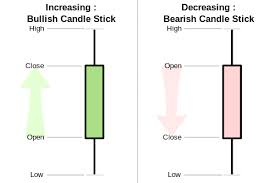
\includegraphics[width=7cm]{chp2_Candlestick}
%\caption{fs yrytrytr}
\caption[Candlestick representation of daily open and close prices]{Candlestick representation of daily open and close prices. Different colouring is used to distinguish between prices going up or down.}
\label{fig:Candlestick}
\end{figure}

Technical analysis via candlesticks is reputed to have been developed by Munelusa Homma, a legendary trader of rice in Osaka, Japan who made a fortune analysing rice prices with candlesticks in the seventeenth century \citep{nison2001japanese}. Candlestick patterns with supposed predictive qualities can be derived from a single day or from considering a few days, usually 2 or 3, together \citep{bigalow2011profitable}. There are a huge number of patterns recorded in the literature and usually assigned exotic names such as \textquotedblleft White Marubozu", "Black Shooting Star" and "Hanging Man". Examples of such named patterns can be seen in Figure \ref{fig:Candlestick_Patterns}.

\begin{figure}[tbph!]
\centering
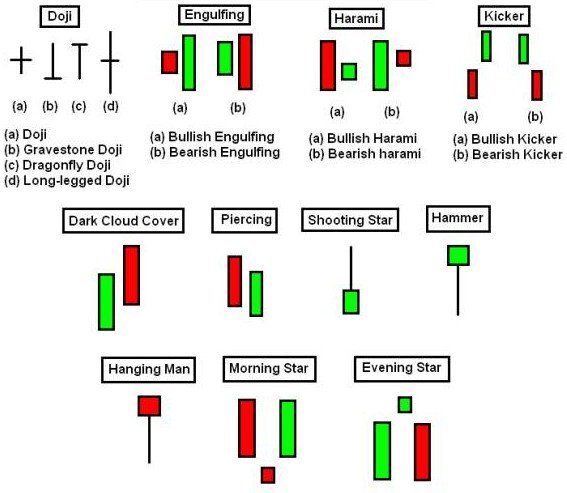
\includegraphics[width=9cm]{chp2_Candlestick_Patterns}
\caption[Examples of well known candlestick patterns]{Examples of well known patterns encountered in candlestick analysis.}
\label{fig:Candlestick_Patterns}
\end{figure}

Candlestick patterns are essentially visualisation tools providing an easy to comprehend view of the market movements in a particular day. However there is some vital information which is not conveyed in a candlestick. In particular the order of events isn't displayed. Figure \ref{fig:chp2_candle_order} shows how two days can produce the same candlestick but in actuality the price movements and volatility in them was very different. Depending upon the type of trading system being employed this could have important effects.

\begin{figure}[tbph!]
\centering
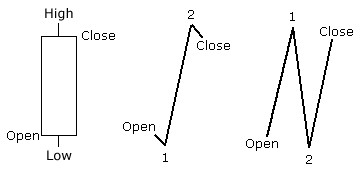
\includegraphics[width=7cm]{chp2_candle_order}
\caption[Candlesticks and market movement]{Candlesticks don't provide information regarding the order of price movements. Both these daily price movements would be represented with the same candlestick pattern.}
\label{fig:chp2_candle_order}
\end{figure}

%11. Candlestick technical trading strategies Can they create value for investors - \cite{Marshall20062303}
As always with technical analysis there is doubt as to the validity of the methods despite its almost universal employment. An in-depth study of the predictive power of a range of candlestick patterns on stock prices between 1992 and 2002 from the Dow Jones Industrial Average (DJIA) was carried out by \citep{Marshall20062303} in which doubt was cast on the validity of candlestick patterns to predict market movements. The workers used a range of bullish (signals that indicate a trader should buy) and bearish (signals that indicate a trader should sell) candlestick patterns to initiate trades on the various stocks. Trades were held for ten days as it was assumed that these patterns reflect short terms trends and thus have a predictive power in a similar time frame. In order to quantify the results generated from the use candlestick patterns they were compared to results observed from four alternative null models. Simulated stock data was generated using a bootstrapping methodology \citep{EfronBootstrapping} and then four null models were applied to the data, random walk, an autoregressive process of order one (AR(1)), a GARCH in-Mean (GARCH-M) model and an Exponential GARCH (EGARCH) model.

From the comparison of the results generated from the candlestick patterns and the four null models the workers concluded that the variety of candlestick patterns tested had no predictive power on the stocks at all. The returns from making buying and selling decisions based on candlestick patterns didn't outperform the null models on the simulated data. As always one has to be slightly careful with results of this nature as the trading period was fixed at ten days, in other words the candlestick patterns were used as an entry signal for the trade but there wasn't an exit signal. Further in reality use of candlesticks analysis would be incorporated into a trading system, which typically consists entry and exit signal, position sizing rules and money management strategies \citep{faith2007way}.

\subsection{Trend Reversal Oscillators}
%6. Adaptive use of technical indicators for the prediction of intra-day stock prices - \cite{TanakaYamawaki2007125}
\cite{TanakaYamawaki2007125} reported the use of several technical analysis techniques in the successful prediction of price movements in eight stocks found on the New York Stock Exchange (NYSE) by analysing tick data. The predictions were in the very short term as tick data is the most granular level reported in financial data. The workers used ten technical analysis indicators from three broad classes, namely trend indicators, oscillators to find market reversals and momentum indicators to measure the strength of the market. Combinations of indicators, typically from the different categories are usually combined by market participants into a variety of systems. In this study the ten indicators can form a possible 1023 combinations. A genetic algorithm was used to determine the best combination of indicators for each stock, resulting in a customised combination for each. Using each stock's indicators, the next ten ticks of data were modelled with very high accuracy, with predictions for IBM's stock being the best at a very impressive 82\%. 

%13. "Intelligent stock trading system based on improved technical analysis and Echo State Network " - \cite{Lin201111347}
%MA, RSI, ROC, stochastics, candle's, - INTERESTING

%14. "Is technical analysis profitable on a stock market which has characteristics that suggest it may be inefficient" - \cite{Marshall2005384}
%NZ Stock mkt - MA, ROC, 

%\subsection{Data Snooping}
%17. The impact of data snooping on the testing of technical analysis: An empirical study of Asian stock markets - \cite{Chen2009580}
%The primary aim of this study is to investigate the validity and predictability of technical analysis in eight Asian equity markets. We employ the bootstrap tests of White (2000) and Hansen (2005) to determine whether any superior trading rule is found to exist amongst the 'universe' of technical trading rules identified by Sullivan et al. (1999). We use these powerful bootstrap tests to ascertain the profitability of technical analysis, along with two institutional adjustments for non-synchronous trading and transaction costs. The empirical results indicate that these three elements, data snooping, non-synchronous trading and transaction costs, have significant impact on the overall performance of technical analysis; indeed, the results for these eight Asian stock markets support the efficient market hypothesis, demonstrating that the generation of economic profits through the use of technical analysis is \textbf{extremely unlikely} with these particular markets.
%
%Earlier paper - \cite{Prodan2013214}

\section{Time Series Analysis}
%19 - 25 years of time series forecasting - \cite{DeGooijer2006443}
The study of forecasting time series data has been an active area of study for several decades and an overview of work over 25 years has been documented by \cite{DeGooijer2006443}. Series data is ordered such that the ordering is an important if not critical aspect of the data and the requirement to maintain this ordering enforces certain constraints on its processing. Series data can be ordered by factors such as distance or height but typically time is the ordering encountered, and thus such collections are referred to as time series. Analysis of time series data is found in a wide range of areas including, Sales Forecasting, Speech Recognition, Economic Forecasting, Stock Market Analysis, Process and Quality Control and Seismic Recordings.

In general with non-series data we are interested in the relationships between the attributes of any particular row of data and perhaps how they affect the parameter we are interested in. Frequently some kind of regression technique is used in this kind of analysis in order to answer questions such as how is rainfall in an area affected by altitude or how does fuel consumption vary with car engine size \citep{han2011data}.

However with time series data there is an additional consideration, the relationship between the attribute's current value to that of its previous or later values. This is known as auto-correlation \citep{mills2011} and more details can be seen in section \ref{sec:autoregression}. Typically with financial data we are interested in previous values, in other words how is today's price of a security affected by the price one, two or three days ago?

As illustrated in Figure \ref{fig:TimeSeriesComponents} a time series can contain some or all of the following components:
\begin{enumerate}
\item Trend - the overall direction of the series, is it increasing or decreasing over time?
\item Seasonality - regular variations in the time series that is caused by re-occurring events, for example a spike in sales during the Christmas period \citep{So2014212}.
\item Random component - additional fluctuations in the series that may be attributed to noise or other random events.
\end{enumerate}

\begin{figure}[tbph!]
\centering
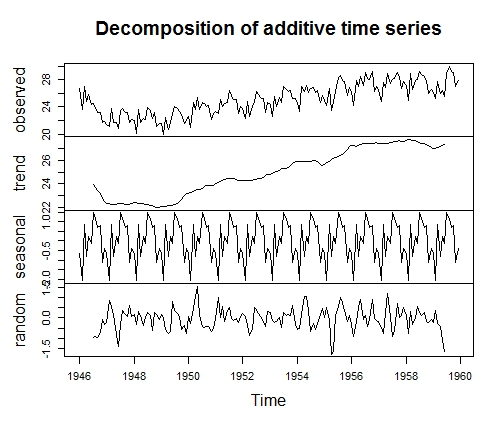
\includegraphics[height=12cm]{chp2_TimeSeriesComponents}
\caption[A time series decomposed into primary components]{A time series decomposed into its three primary components.}
\label{fig:TimeSeriesComponents}
\end{figure}

There are three primary types of time series, stationary, additive and multiplicative. Stationary series have constant amplitude without a trend element and an example can be seen in Figure \ref{fig:Stationary_ts}. Often stationary time series are repetitive, in other words showing constant auto-correlation and are considered the easiest type to model. A stationary time series can be composed of a seasonal element and/or a random component, thus:

\begin{center}
\textit{stationary time series = seasonality +/or noise}
\end{center}

\begin{figure}[tbph!]
\centering
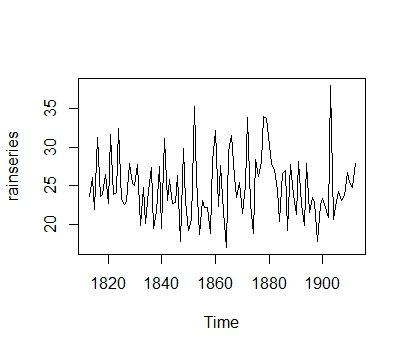
\includegraphics{chp2_Stationary_ts}
\caption[A stationary time series]{Example of a stationary time series which can be made up from noise and/or a seasonal component.}
\label{fig:Stationary_ts}
\end{figure}

The second type of time series is the additive type. In this type all three components of the series are present, trend, seasonality and noise. The distinguishing feature here is the amplitude of the seasonal component in that it is quite regular being static over time. An example of an additive series can be seen in Figure \ref{fig:Add2_ts}. This time series is trending upwards overall but there is a clear repetitive pattern of peaks and troughs caused by the seasonality, with the heights of the peaks all being similar. We can consider an additive time series as:

\begin{center}
\textit{additive time series = trend + seasonality + noise}
\end{center}

\begin{figure}[tbph!]
\centering
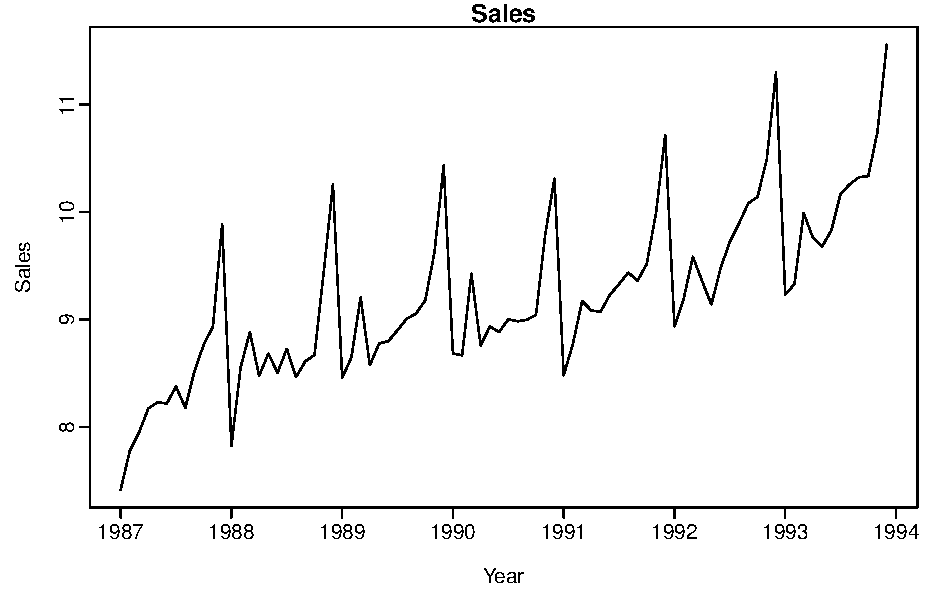
\includegraphics{chp2_Add2_ts}
\caption[An additive time series]{Example of an additive time series which results from all three components trend, noise and seasonality.}
\label{fig:Add2_ts}
\end{figure}

The third type of time series, as seen in Figure \ref{fig:Multi_ts} is multiplicative. This is similar to the additive version except the amplitude of the seasonality increases over time. It can be considered as:

\begin{center}
\textit{multiplicative time series = trend * seasonality * noise}
\end{center}

\begin{figure}[tbph!]
\centering
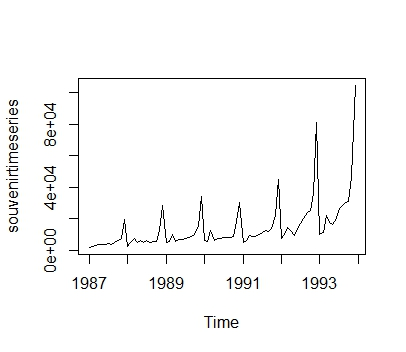
\includegraphics{chp2_Multi_ts}
\caption[A multiplicative time series]{Example of a multiplicative time series resulting from the effects of trend, noise and seasonality.}
\label{fig:Multi_ts}
\end{figure}

Financial time series can be considered as containing all three elements of a time series. They can show properties of a stationary time series when they are range bound and only move between two values. At other times, markets trend strongly consistently, making new highs or lows and exhibit properties of an additive and occasionally a multiplicative series.

\subsection{Time Series Smoothing}
\label{sec:expsmoothing}
Smoothing is an important and widely adopted method to predict financial markets.  Recent work on smoothing time series data has its origins in \cite{brown1959statistical}, \cite{brown1963statistical}, \cite{Holt20045} and \cite{Winters1960}. Typically, the various smoothing techniques encountered are based around the concept of moving averages. This section will introduce a variety of smoothing methods commonly encountered in forecasting financial data. 

\subsubsection{Simple Moving Average (SMA)}
\label{sec:chp2_sma}
A simple moving average is calculated from the value itself and its neighbours, which can be ahead or behind in the series. In this study values behind the current value are considered. The number of previous values included is often referred to as the \textquotedblleft window" or \textquotedblleft lag", so if one was to consider the current value and four previous ones this would be considered a simple moving average of lag 5 (SMA5). An example of a simple moving average can be seen in Table \ref{tab:SMA}, where a SMA5 of the closing price has been added.

% Table generated by Excel2LaTeX from sheet 'Pairs'
\begin{table}[htbp]
  \centering
  \caption[Example of a Simple Moving Average]{Example of a simple moving average of the closing price with a lag of 5 periods.}
    \begin{tabular}{@{\extracolsep{5pt}}lccccc}
    \toprule
    \textbf{Date} & \textbf{Open} & \textbf{High} & \textbf{Low} & \textbf{Close} & \textbf{SMA5} \\
    \midrule
    02/01/14 & 9598  & 9621  & 9394  & 9400  &  NA \\
    03/01/14 & 9410  & 9453  & 9368  & 9435  &  NA \\
    06/01/14 & 9419  & 9469  & 9400  & 9428  &  NA \\
    07/01/14 & 9446  & 9519  & 9417  & 9506  &  NA \\
    08/01/14 & 9513  & 9516  & 9468  & 9498  & 9453 \\
    09/01/14 & 9492  & 9550  & 9403  & 9422  & 9458 \\
    10/01/14 & 9474  & 9530  & 9441  & 9473  & 9465 \\
    13/01/14 & 9498  & 9519  & 9457  & 9510  & 9482 \\
    \bottomrule
    \normalsize 
    \end{tabular}%
  \label{tab:SMA}%
\end{table}%

\subsubsection{Weighted Moving Average (WMA)}
A simple moving average assigns equal importance to all data points being averaged, however if this is considered unsuitable a higher weighting can be applied to certain data points elevating their importance in the average and thus generating a weighted moving average \citep{WMA2}. Typically the more recent data points in a time series would be given higher importance. One common version of a WMA is to decrease the weighting by one for each period in the average. The formula for calculating a weighted moving average is:

\[ ((n*P_{n}) + (n-1*P_{n-1})+ ... (n-(n-1)*P_{n-(n-1)})) \div (n + (n-1) + ... n-(n-1))\]

where: \\
$ n $ = the number of periods used in calculating the moving average \\
$ Pn $ = the price of the most recent period used to calculate the moving average 

An extra column has been added to the data in Table \ref{tab:SMA} which contains the WMA for the last five close values. The current value was multiplied by 5, the previous one by 4, the previous one to that by 3 and so on. These five values were added together and divided by 5+4+3+2+1 to generate the WMA as shown in Table \ref{tab:WMA}.

% Table generated by Excel2LaTeX from sheet 'Pairs'
\begin{table}[htbp]
  \centering
  \caption[Example of a Weighted Moving Average]{Example of a weighted moving average.}
    \begin{tabular}{ccccccc}
    \toprule
    \textbf{Date} & \textbf{Open} & \textbf{High} & \textbf{Low} & \textbf{Close} & \textbf{SMA5} & \textbf{WMA5} \\
    \midrule
    02/01/14 & 9598  & 9621  & 9394  & 9400  &  NA   & NA  \\
    03/01/14 & 9410  & 9453  & 9368  & 9435  &  NA   & NA \\
    06/01/14 & 9419  & 9469  & 9400  & 9428  &  NA   & NA \\
    07/01/14 & 9446  & 9519  & 9417  & 9506  &  NA   & NA \\
    08/01/14 & 9513  & 9516  & 9468  & 9498  & 9453  & 9471 \\
    09/01/14 & 9492  & 9550  & 9403  & 9422  & 9458  & 9461 \\
    10/01/14 & 9474  & 9530  & 9441  & 9473  & 9465  & 9466 \\
    13/01/14 & 9498  & 9519  & 9457  & 9510  & 9482  & 9481 \\
    \bottomrule
    \end{tabular}%
  \label{tab:WMA}%
\end{table}%

\subsubsection{Exponential Moving Average (EMA)}
An exponential moving average (EMA) is an extension of the weighted moving average \citep{Ord20041}. In comparison to the simple moving average, greater emphasis is given to the most recent data points and the resulting averaged values are closer to the actual observations of the data set. Weighting factors decay exponentially resulting in the emphasis falling on the recent values though not discarding the older ones totally. 

\subsubsection{Moving Averages in Practical Use }
Moving averages are widely used in the financial world to predict the start of trends which is important as trends are considered the best opportunity to make profits from the markets. By their nature moving averages are lagged indicators in that they reflect market action from the past (recent or distant depending on the lag variable) and this can be considered a drawback. The lag period offers a trade off in terms of prediction. If the lag is short and/or weighting is applied the average is affected strongly by recent prices and trends can be detected in the early stages and trading profits can be enhanced. However when the average is close to the current price they have a tendency to generate \textquotedblleft false signals" (see section \ref{sec:tradingsystems} for an explanation of entry and exit signals), in other words prices may start to rise (or fall) but they are not actually in a trend, it is just the natural wax and wane of the market, and traders are said to be \textquotedblleft whipsawed". When the lag variable is long a different problem is encountered. For example, if a price moves above a long moving average the indicated trend is usually genuine, however by the time this is reflected in the average a lot of the trend has developed and the trader has lost a lot of potential profits. Thus there are pros and cons associated with using the different types of moving average.

\subsubsection{Holt-Winters Smoothing Models}
\label{sec:holtwinters}
The exponential smoothing of a time series containing noise, trend and seasonality was developed by \cite{Winters1960} who as a student of Holt, built upon his previous work, and is today called the Holt-Winters method. This method uses three parameters alpha, beta and gamma which define the degree of smoothing to be applied to the three components of the time series. Firstly, a value of alpha is used to dictate the amount of smoothing to apply, with high smoothing factors placing more emphasis on recent data points at the expense of those further away. In a data set with trend this simple exponential moving average doesn't perform well and a second order of smoothing is needed, so called \textquotedblleft double exponential smoothing". The parameter beta in Holt-Winters defines this second order smoothing. Finally, if a seasonal component is also present in the data set a third level of smoothing is introduced making the process a triple exponential smoothing. It is this third level of smoothing that the parameter gamma refers to. Depending upon the nature of the time series one, two or all three of the parameters may be defined in the Holt-Winters methodology.

If researching a time series with no seasonality or trend use of the Holt-Winters model with the beta and gamma parameters set to false, in other words not used, is appropriate. Figure \ref{fig:HW1a} shows the addition of an exponential smoothing line to the stationary data set introduced in Figure \ref{fig:Stationary_ts}.

%\begin{figure}[tbph!]
%\centering
%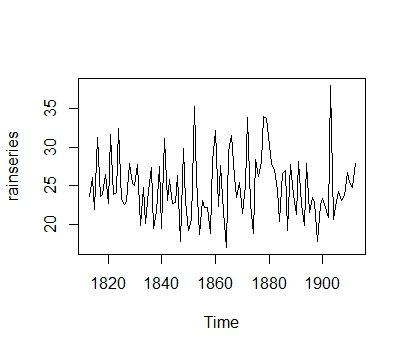
\includegraphics[width=8cm]{chp2_HW1}
%\caption[A time series with no seasonality or trend]{For a time series with no seasonality or trend, the use of Holt-Winters exponential smoothing with the beta and gamma parameters set to false is appropriate.}
%\label{fig:HW1}
%\end{figure}

\begin{figure}[tbph!]
\centering
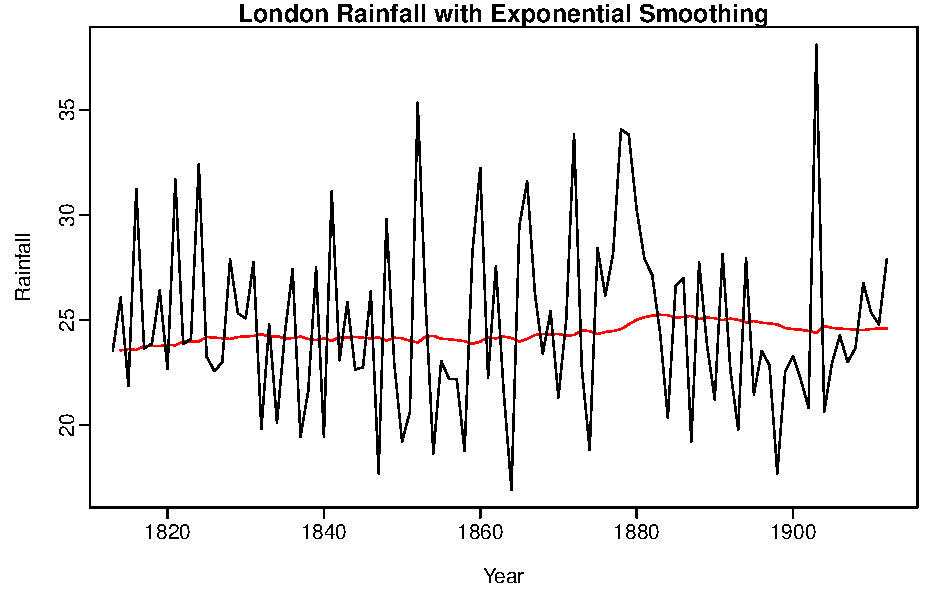
\includegraphics{chp2_HW1a}
\caption[Exponential smoothing of a time series with no seasonality or trend]{A time series with no seasonality or trend, showing the fitted line generated from Holt-Winters exponential smoothing with the beta and gamma parameters set to false.}
\label{fig:HW1a}
\end{figure}

If the time series is additive with a trend but without seasonality the use of Holt-Winters with values used for alpha and beta but with the gamma parameter set to false is appropriate. Such a time series can be seen in Figure \ref{fig:HW2a} with the exponential smoothing. Finally if the time series contains all three components a smoothing line can be fitted using Holt-Winters exponential smoothing in which there are values for all three terms alpha, beta and gamma. Figure \ref{fig:HW3a} is an example of a time series with both trend and seasonality and overlaid with Holt-Winters smoothing generated by using values for all three terms in the smoothing algorithm.

%\begin{figure}[tbph!]
%\centering
%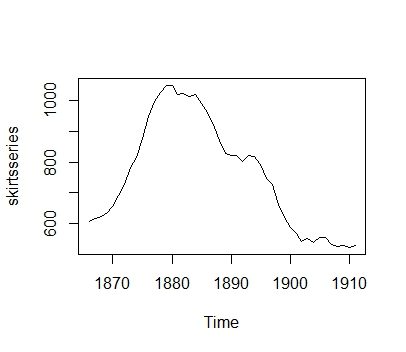
\includegraphics[width=8cm]{chp2_HW2}
%\caption[A time series with trend though no seasonality]{For a time series with trend but no seasonality, the use of Holt-Winters exponential smoothing with the gamma parameter set to false is appropriate.}
%\label{fig:HW2}
%\end{figure}

\begin{figure}[tbph!]
\centering
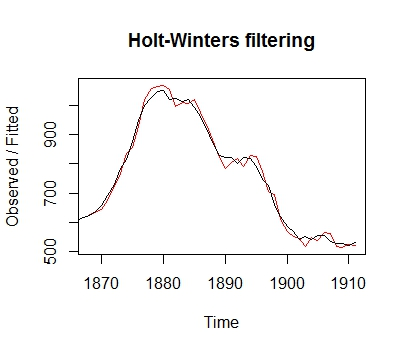
\includegraphics{chp2_HW2a}
\caption[Exponential smoothing of a time series with trend though no seasonality]{A time series with trend though no seasonality, showing the fitted Holt-Winters exponential smoothing with the gamma parameter set to false.}
\label{fig:HW2a}
\end{figure}

%\begin{figure}[tbph!]
%\centering
%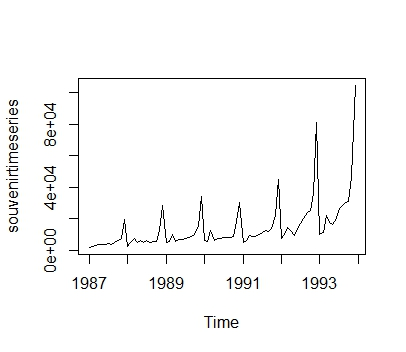
\includegraphics[width=8cm]{chp2_HW3}
%\caption[A time series with trend and seasonality]{For a time series with trend and seasonality, the use of Holt-Winters exponential smoothing is appropriate.}
%\label{fig:HW3}
%\end{figure}

\begin{figure}[tbph!]
\centering
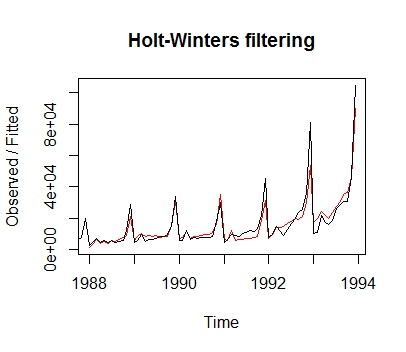
\includegraphics{chp2_HW3a}
\caption[Exponential smoothing of a time series with trend and seasonality]{A time series with trend and seasonality, showing the fitted Holt-Winters exponential smoothing.}
\label{fig:HW3a}
\end{figure}


%%29 - Holt’s exponential smoothing and neural network models for forecasting interval-valued time series " - \cite{Maia2011740}

\subsection{Auto-Regression Family of Models}

\subsubsection{Auto-Regression}
\label{sec:autoregression}
Regression is the study of the impact of known variables (independent) on an unknown (dependent) variable and addresses questions such as how does a person's income vary with their years of education. The general equation for linear regression is given by:
\[ y = a + bx + \varepsilon \]
where:\\
$ a $ is the intercept.\\
$ b $ is the co-efficient.\\
$ x $ is the independent variable.\\
$ \varepsilon $ is the error term.

In reality there are often a large number of independent variables that affect the unknown under study and thus multiple regression, shown below, is usually of interest.
\[ y_{1} = a + b_{1}x_{1i} + b_{2}x_{2i} +  ....   +b_{n}x_{ni} + \varepsilon\]
In a time series the preceding values often have a bearing on the current data point, and this is especially important in financial time series data. Thus auto-regression is the prediction of the current point from the use of previous values of the data point itself, and is given by:
\[ t_{t}=c+b_{1}*r_{t-1}+b_{2}*r_{t-2}...b_{p}*r_{t-p}+ \varepsilon \]

where:\\
$ c $ is the intercept, is often zero and the mean of the time series. \\
$ b_{1}-b_{p} $ are the independent variables, the previous values.\\
$ \varepsilon $ is random noise. 

\subsection{Auto-Regressive Moving Average (ARMA)}
\label{sec:arma}
The auto-regressive moving average (ARMA)model, also known as Box-Jenkins \citep{box1970time}, combines moving averages with auto-regression. A model that uses moving averages to predict current values is given by:

\[ -r_{t}=c+a_{1}*ma_{t-1}+a_{2}*ma_{t-2}...a_{q}*ma_{t-q}+err_{t}\]

ARMA combines the moving average model with auto-regressive terms to generate:

%\[ r(t) =   c+
%			b_{1}*r_{t-1}+b_{2}*r_{t-2}...b_{p}*r_{t-p}+ 
%			a_{1}*ma_{t-1}+a_{2}*ma_{t-2}...a_{q}*ma_{t-q} 
%			+err \]

\begin{align*}
	r(t) & =   c+ \\
    	 & b_{1}*r_{t-1}+b_{2}*r_{t-2}...b_{p}*r_{t-p}+ \\ 
      	 & a_{1}*ma_{t-1}+a_{2}*ma_{t-2}...a_{q}*ma_{t-q} \\
    	 & +err
\end{align*}

where:\\
$ c $ is the intercept, which is often zero and the mean of the time series. \\
$ b_{1}-b_{p} $ are the independent variables, the previous values in the auto-regression term.\\
$ a_{1}-a_{p} $ are parameters of the moving average model.\\
$ \varepsilon $ is random noise.

An ARMA(1,1) model uses the previous value in the auto-regression term and the previous value's moving average. Thus in general terms an ARMA(p,q) model uses the previous p values in the auto-regression term and the moving averages derived from the last q values. There are therefore three steps in in developing an ARMA model:
\begin{enumerate}
\item identification step in which the order of AR and MA components is determined
\item parameter estimation
\item forecasting
\end{enumerate}

ARMA models have certain intrinsic properties that may be considered drawbacks, namely the requirement for the time series to be stationary with no trend and also linear and the difficulty in deriving the correct parameters to use in the model. In order to overcome these restrictions researchers have tried a number of approaches to enhance the effectiveness of ARMA models.

The problem of model and parameter selection in ARMA models has also been addressed by \cite{Rojas2008519}. The authors make the point that in traditional research choosing the correct model is time consuming and requires a large degree of expertise. In order to circumvent these issues they propose an automatic model selection method to speed up the process, remove the need for expert intervention and allow the processing of a large number of time series. In a similar study \cite{Qian20076180} investigate how to determine model selection where there are potentially millions of candidate ARMA models available for the time series. Again, the authors propose an automatic selection algorithm centred on the Gibbs sampler. The proposed method allows for various problems typically encountered in selecting ARMA models and the resulting choice was used to generate a prediction of China’s Consumer Price Index (CPI).

\subsection{Auto-Regressive Integrated Moving Average (ARIMA)}
\label{sec:arima}
One limitation with the ARMA model and indeed other approaches is that it is assumed that the time series is stationary, it doesn't have trend and has constant variance and mean \citep{shumway2010time}. In reality of course many time series data sets have trend, and in the world of financial data this is also true. In order to account for trend in a time series it is often transformed into a stationary data set, modelling is then performed on this adapted data after which it is returned to its original state. In effect the trend aspect is removed, modelling is done, then the trend component is added back into the data.

One such method for removing trend is differencing \citep{mills2011}. Differencing is the technique of replacing the actual values of the observations with the values of the differences between them. This is represented as:

\[ Diff1_{t}=r_{t}-r_{t-1} \]

Differencing is the same as calculating the derivative of the series, thus a time series that has under gone differencing is considered \textquotedblleft integrated". If taking this so-called first difference doesn't remove the trend one can go further and use the second difference:

\[ Diff2_{t}=(r_{t}-r_{t-1})-(r_{t-1}-r_{t-2}) \]

Addition of an integration step to the ARMA model results in an auto-regressive integrated moving average (ARIMA) model, with the general formula:

%\begin{gather*}
%	r(t) =   c+ \\
%    b_{1}*r_{t-1}+b_{2}*r_{t-2}...b_{p}*r_{t-p}+ \\ 
%    a_{1}*ma_{t-1}+a_{2}*ma_{t-2}...a_{q}*ma_{t-q} \\
%    +err
%\end{gather*}

\begin{align*}
	r(t) & =   c+ \\
    & b_{1}*r_{t-1}+b_{2}*r_{t-2}...b_{p}*r_{t-p}+ \\ 
    & a_{1}*ma_{t-1}+a_{2}*ma_{t-2}...a_{q}*ma_{t-q} \\
    & d_{1}*diff_{t-1}+d_{2}*diff_{t-2} ... d_{d}*diff_{t-d} \\
    & +err
\end{align*}

where:

$ c $ is the intercept, which is often zero and the mean of the time series.

$ b_{1}-b_{p} $ are the independent variables, the previous values in the auto-regression term.

$ a_{1}-a_{p} $ are parameters of the moving average model.

$ d_{1}-_{p} $ are the parameters of the differencing term.
$ \varepsilon $ is random noise.


ARIMA models are usually referenced as ARIMA(p,d,q) with p the number of terms used in the auto-regression, d the number of differencing terms and q the number of terms used in the moving average. A summary of which model (Holt-Winters, ARMA or ARIMA) to use with which type of time series can be seen in Table \ref{tab:tsmodelsummary}.

\begin{table}[htbp]
  \centering
  \caption[Times series and matching models]{Appropriate models for use with time series data.}
    \begin{tabular}{@{\extracolsep{5pt}}ccccc}
    \toprule
    \textbf{Model} & \textbf{\parbox[t]{3cm}{\centering Time Series\\Required}} & \textbf{\parbox[t]{3cm}{\centering Assumes\\Correlation}} & \textbf{Trend} & \textbf{Seasonality} \\
    \midrule
    Holt-Winters & Short Term  & N  & Y  & Y \\
    ARMA & Stationary  & Y  & N  & Y \\
    ARIMA & \parbox[t]{3cm}{\centering Non-stationary:\\Additive or\\Multiplicative}  & Y  & Y  & Y \\
    \bottomrule
    \normalsize 
    \end{tabular}%
  \label{tab:tsmodelsummary}%
\end{table}

\subsection{ARIMA Parameter Selection}
\label{sec:acf}
An important aspect of building time series models with ARIMA techniques is the choice of parameters to use. Auto-correlation (AC) and partial auto-correlation (PAC) are important measures in the selection process of these parameters \citep{mills2011}. 

Correlation is the measure of how one variable changes with a second one. For example if variable A increases while variable B increases they are positively correlated and conversely they are negatively correlated when one decreases as the other increases. Further, correlations are measured by degree on a scale of 1 to -1, with 1 being perfectly correlated. A value of 1 indicates that the two variables increase together perfectly in sync, whereas a value of -1 suggests that as one variable increases the other decreases by the same amount. Finally a value of 0 is indicative of no correlation at all between the two variables.

Auto-correlation is the correlation between an attributes value now and the same attribute's value in the past or future \citep{shumway2010time}. Typically with financial data we are interested in the correlation with values in the past. The interval between the value of interest and the previous observation used in determining the correlation is known as the lag. Thus the correlation between the current observation and the previous one may be of interest, and this is a lag of +1, while a value five time intervals previous is +5. Non-intuitively positive values for lags refer to the past while negative values are in the future. 

A correlogram is a matrix plot of auto-correlations over a series of time lags.  Correlograms are used in checking data for randomness and in the model identification stage of the ARMA methodology (see section \ref{sec:arma}). Data is considered random if the auto-correlation value is close to zero.  In general a data set's randomness needs to be checked in order to confirm the validity of many statistical tests. Thus a correlogram helps to determine if data is random or if an observation is related to an earlier one, thereby helping in the determination of an appropriate ARMA model. Figure \ref{fig:acf80} is the correlogram of auto-correlation and Figure \ref{fig:pacf} the correlogram of partial auto-correlation for a data set of rain fall figures.

%and Figure \ref{fig:pacf} is the correlogram of the seasonal component of this data set.

\begin{figure}[tbph!]
\centering
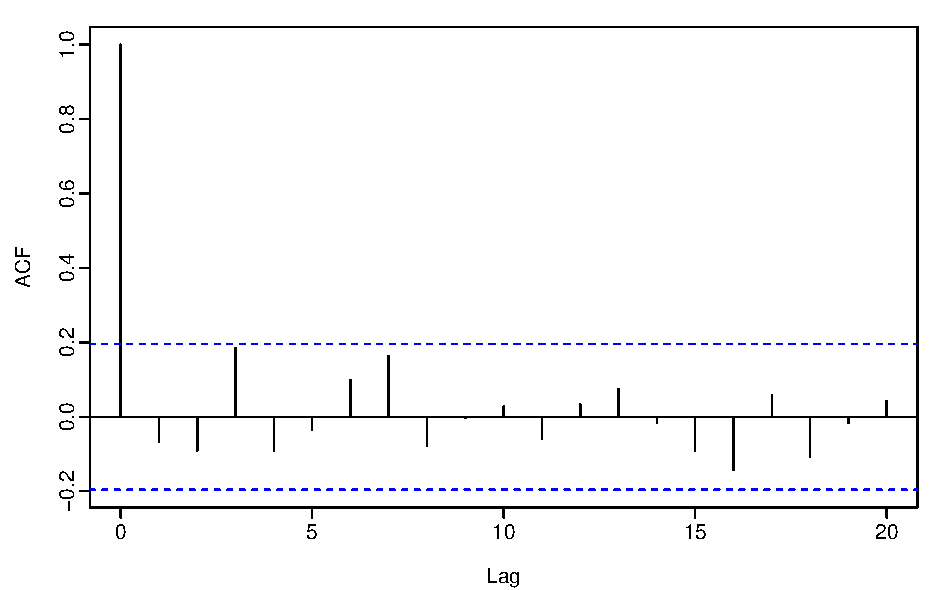
\includegraphics{chp2_acf80}
\caption[Correlogram of auto-correlations]{Correlogram of auto-correlations.}
\label{fig:acf80}
\end{figure}

\begin{figure}[tbph!]
\centering
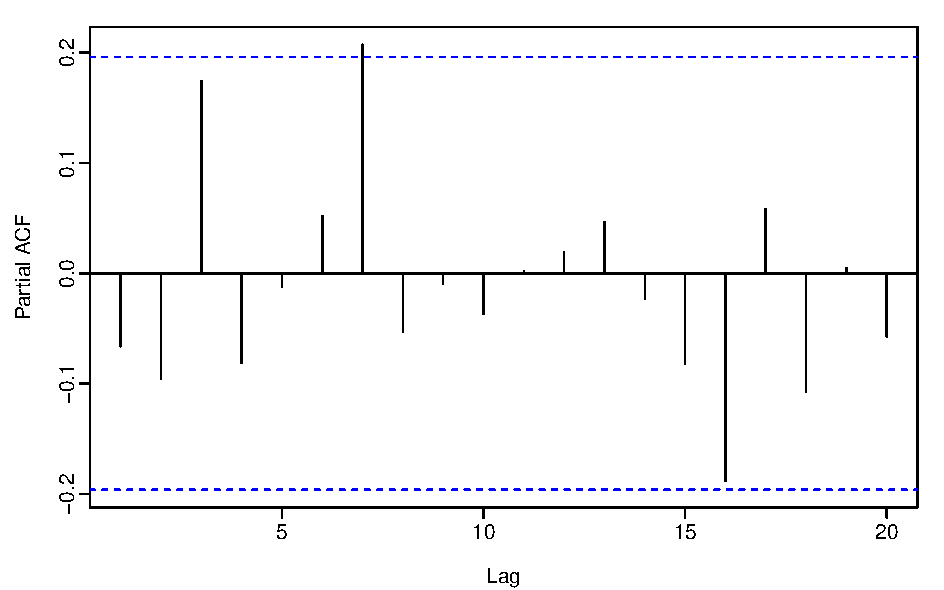
\includegraphics{chp2_p_pacf}
\caption[Correlogram of partial auto-correlations]{Correlogram of partial auto-correlations.}
\label{fig:pacf}
\end{figure}

The partial correlation is defined as the degree of correlation not already explained by the correlations previously measured. If the regression of variable A on variables B1, B2 and B3 is considered the partial correlation between variables A and B3 is the degree of correlation not accounted for by their common correlations with variables B1 and B2. In a similar manner the partial autocorrelation is the unexplained correlation after considering the variable and itself at an earlier time period. In a series, if a variable A at time t is correlated with an earlier lag at time t-1 it follows that the variable at t-1 itself is correlated with the previous variable at lag t-2. By extension the variable at time t should also be correlated with the variable at lag t-2, as the correlation will propagate through the series. The partial autocorrelation is the difference the expected correlations due the propagating factors and the actual correlation measured.

If the ARIMA model is ARIMA(p,d,0) or ARIMA(0,d,q) then the ACF and PACF plots are helpful in deciding the values for p or q. If both p and q are positive, the ACF and PACF are not useful in estimating the values for p and q. An ARIMA(p,d,0) model may be appropriate if the ACF and PACF plots of the stationary data exhibit an exponentially decaying pattern in the ACF and a large spike at lag p in PACF plot. Conversely an ARIMA(0,d,q) model may be appropriate if the PACF is decaying exponentially and there is there is a significant spike in the ACF plot at lag q.

\subsection{Hybrid Models}
Auto-regressive (integrated) moving average models have shown themselves to be important modelling methods for time series data, including financial time series data. However the techniques have limitations that have detracted from their popularity, namely their assumption of a linear relationship and the need for a lot of data to produce accurate results. In order to address these limitations a variety of hybrid solutions have been proposed in which ARIMA models are combined with other techniques, often non-linear prediction algorithms \citep{Wang2012758,Khashei20124344,Aladag20091467}.

% ARIMA / ANNs
One combination that has found a lot of attention in the literature is the combination of Artificial Neural Networks (ANNs) with ARIMA. \cite{Khashei2009956} report on the use of this combination in a attempt to predict the future price movement in gold and US dollar / Iran rials financial markets. The workers report favourable results in comparison to the techniques alone and suggest the method as having potential for accurate predictions of non-linear time series data. In a similar study \cite{Zhang2003159} applied a combination of ARIMA and ANN to various data sets including the British pound / US dollar exchange rate. They observe that in the literature in general these two popular techniques are frequently compared in terms of predictive power with the reported results non-conclusive. Results from the three data sets modelled show that the combination of the two methods outperform the individual ones when the mean squared error (MSE) and mean
absolute deviation (MAD) are used as the measure of forecasting accuracy.

\cite{Fatima20082742} also investigated the impact of a hybrid approach in modelling short term predictions for the Karachi Stock Exchange index (KSE100). The authors reported comparison results for ANN versus ARIMA and a hybrid of ANN/ARIMA. The hybrid solution out-performed the individual ARIMA and ANN models. It is postulated that a rationale for this is that at any point in time financial markets are subject to linear, non-linear and volatility patterns as the cumulative effects of government fiscal and monetary policies and general rumour and political instabilities feed into the market. Under these complex conditions simple models can only capture one aspect of the underlying factors affecting the price series. A hybrid combination approach is more successful as more of the market variance is modelled.

% ARIMA / WAVELETS
\cite{Kriechbaumer201432} reports on a further hybrid approach to forecast the prices of aluminum, copper, lead and zinc. Previous research has indicated that these markets exhibit a strong cyclic behaviour. In an attempt to factor this into the predictive model ARIMA was coupled with a wavelet approach. Wavelet analysis decomposes a time series into its frequency and time domains in an attempt to isolate this cyclic behaviour. The performance of the ARIMA modelling was shown to be enhanced substantially by the addition of wavelet based multi-resolution analysis (MRA) before performing the ARIMA analysis.

\cite{Tan20103606} have also reported the combination of wavelet analysis and ARIMA in the prediction of electricity prices. The general method employed is to transform the original time series data set into a collection of sub-series through the application of wavelet analysis. Subsequent to the transformation a prediction for each sub-series can be made with ARIMA modelling. The final forecasted result is obtained by reforming the sub-series back into the original time series. The authors report results showing the enhanced predictive power of the ARIMA wavelet hybrid approach compared to ARIMA and GARCH models used in isolation.

% ARIMA / SVM
\cite{Pai2005497} reported on attempts to overcome the limitation of ARIMA models in that the time series must be linear by use of an hybrid ARIMA / Support vector machine (SVMs) combination. SVMs have been successfully applied to to non-linear regression problems and the authors have harnessed the strengths of both methodologies in order to predict the prices of a selection of fifty stocks. Results from the work show that the hybrid method out-performs the ARIMA and SVM methods individually.

\cite{Rout20147} report the use of ARMA models in the prediction of exchange rates. The workers note the limitations of ARMA in that the time series data must be linear and stationary, a condition often not met in practical situations and the difficulty in deriving steps one and two (listed previously) in developing the ARMA model. In order to overcome these limitations ARMA is combined with differential evolution (DE) in order to determine the models feed-forward and feed-back parameters. The results from the prediction models generated are compared with models resulting from ARMA in conjunction with particle swarm optimisation (PSO), cat swarm optimisation (CSO), bacterial foraging optimization (BFO) and forward backward least mean square (FBLMS). The workers conclude that the ARMA - DE model produces the best short and long-range predictions from the options tested and is a potentially valuable method in predicting exchange rates on the international finance markets.

%ARIMA/GARCH
%34 - International evidence on crude oil price dynamics: Applications of ARIMA-GARCH models - \cite{Mohammadi20101001}

%20 - Forecasting aggregate retail sales:: a comparison of artificial neural networks and traditional methods - \cite{Alon2001147}
%Looks at various time series models, good overview.
 
%\subsection{Seasonality}

%28 -Dynamic seasonality in time series - \cite{So2014212}

%\subsection{Data Mining of Time Series Data}
%21 - A review on time series data mining - \cite{Fu2011164}
%%Time series is an important class of temporal data objects and it can be easily obtained from scientific and financial applications. A time series is a collection of observations made chronologically. The nature of time series data includes: large in data size, high dimensionality and necessary to update continuously. Moreover time series data, which is characterized by its numerical and continuous nature, is always considered as a whole instead of individual numerical field. The increasing use of time series data has initiated a great deal of research and development attempts in the field of data mining. The abundant research on time series data mining in the last decade could hamper the entry of interested researchers, due to its complexity. In this paper, a comprehensive revision on the existing time series data mining research is given. They are generally categorized into representation and indexing, similarity measure, segmentation, visualization and mining. Moreover state-of-the-art research issues are also highlighted. The primary objective of this paper is to serve as a glossary for interested researchers to have an overall picture on the current time series data mining development and identify their potential research direction to further investigation.


%\subsubsection{Neural Nets}
%
%I. Kaastra, M. Boyd, Designing a neural network for forecasting financial and
%economic time-series, Neurocomputing 10 (1996) 215–236.
%
%3 - The use of data mining and neural networks for forecasting stock market returns - \cite{Enke2005927}
%%
%6 - Intelligent technical analysis based equivolume charting for stock trading using neural networks - \cite{Chavarnakul20081004}
%
%23 - A neural-network-based nonlinear metamodeling approach to financial time series forecasting - \cite{Yu2009563}

%\subsubsection{SVM}
%5 - Forecasting stock market movement direction with support vector machine - \cite{Huang20052513}
%
%7 - Financial time series forecasting using support vector machines - \cite{Kim2003307}
%
%\subsubsection{SOM}
%8 - A two-stage architecture for stock price forecasting by integrating self-organizing map and support vector regression - \cite{Hsu20097947}
%%
%9 - A hybrid procedure for stock price prediction by integrating self-organizing map and genetic programming - \cite{Hsu201114026}
% 
%\subsubsection{Clustering}
%10 - Clustering of financial time series - \cite{DUrso20132114}
%
%22 - Clustering of time series data—a survey - \cite{WarrenLiao20051857}
%
%%
%%\subsubsection{Decision Trees}
%%
%11 - Trend discovery in financial time series data using a case based fuzzy decision tree " - \cite{Chang20116070}
%%
%%
%12 - Evolving and clustering fuzzy decision tree for financial time series data forecasting "  - \cite{Lai20093761}

%\subsection{ARCH/GARCH}
%
%ARCH introduced by \cite{Engle} 
%
%GARCH introduced in \cite{TaylorGARCH}
%
%GARCH survey \cite{BollerslevGARCH}



%12 - A nonparametric GARCH model of crude oil price return volatility " - \cite{Hou2012618}
%
%"Volatility in crude oil futures: A comparison of the predictive ability of GARCH and implied volatility models " - \cite{Agnolucci2009316}

%\subsection{Hybrid Approaches}
%
%24 - A new class of hybrid models for time series forecasting - \cite{Khashei20124344}
%
%25 - An artificial neural network (p, d, q) model for timeseries forecasting - \cite{Khashei2010479}
%
%26 - Forecasting nonlinear time series with a hybrid methodology - \cite{Aladag20091467}
%
%27 - Stock index forecasting based on a hybrid model " - \cite{Wang2012758} - GOOD

%\subsection{Comparison of Approches}
%
%AR - 30 - Forecasting models for interval-valued time series " - \cite{Maia20083344}
%
%Neural network and traditional time series
%techniques have been compared in several studies. Sharda
%and Patil [29] found that neural networks performed as good as
%the automatic Box–Jenkins procedure. Maier and Dandy [23]
%suggest that the ARIMA model is better suited for short-term
%forecasts and that neural networks are better suited for longerterm
%forecasts.
%
%R. Sharda, R. Patil, Neural networks as forecasting exports: an empirical test,
%in: Proceedings of IJCNN Meeting 1990 2, 1990, pp. 491–494.
%
%H.R. Maier, G.C. Dandy, Neural network models for forecasting univariate time
%series, Neural Networks World 6 (5) (1996) 747–772.


%\subsubsection{Commodities}
%12a - Forecasting volatility of crude oil markets " - \cite{Kang2009119}
%%
%14 - Modeling and forecasting petroleum futures volatility " - \cite{Sadorsky2006467}



 
% Chapter 3

\chapter{Methodology} % Main chapter title

\label{Chapter3} % For referencing the chapter elsewhere, use \ref{Chapter1} 

\lhead{Chapter 3. \emph{Methodology}} % This is for the header on each page - perhaps a shortened title

%----------------------------------------------------------------------------------------
\section{Data Collection and Quality}
The data used in this study was freely collected from the Yahoo finance web site (www.yahoo.com). It is of high quality with no missing values and represents the opening, high, low and closing prices for each day that the particular market indice was open for trading. 

\section{Data Description}
Data from a variety of national stock market indices was employed in this study. The indices were from a variety of geographic locations with FTSE (UK), DAX (Germany) and CAC (France) all being in Europe, the Dow is from the US, the Nikkei from Japan and AORD from Australia. The data is in the form of so-called daily OHLC (daily open, high, low and close prices) for Monday to Friday (excluding appropriate national holidays) for the period 2000 until the end of 2013. A schematic representation of daily OHLC data can be seen in Figure \ref{fig:chp3_ohlc}. The first six observations from the DAX data set (German national indice) can be seen in Table \ref{tab:daxhead}.

%------------------- Graph of OHLC ---------------------------------
\begin{figure}[tbh]
\centering
%\includegraphics[width=6cm]{../Figures/chp3_ohlc}
\includegraphics[width=6cm]{chp3_ohlc}
\caption[Open, high, low and closing prices (OHLC).]{A schematic representation of open, high, low and closing prices (OHLC).}
\label{fig:chp3_ohlc}
\end{figure}

The final six observations from the DAX data set can be seen in Table \ref{tab:daxtail}. Over the period of the data (2000 until the end of 2013) the DAX started at 6691 and finished at 9552. Summary statistics for the DAX data set can be seen in Table \ref{tab:daxsum}. The data set contains 3621 observations and the closing price has ranged between 2202 and 9742 over the period. A graph of the closing prices from 2000 to 2013 and be seen in Figure \ref{fig:Dax2000_2013} and a graph for 2013 can be seen in Figure \ref{fig:Dax2013}.

%------------------- Table of 1st 6 rows of DAX ---------------------------------


%label - tab:daxhead
% latex table generated in R 3.1.0 by xtable 1.7-3 package
% Wed May 28 17:43:16 2014
\begin{table}[ht]
\centering
\caption[First 6 rows of the Dax data set.]{First 6 rows of the Dax data set} 
\label{tab:daxhead}
\begin{tabular}{lcccc}
  \toprule Date & Open & High & Low & Close \\ 
  \midrule 03/01/2000 & 6962 & 7159 & 6721 & 6751 \\ 
  04/01/2000 & 6747 & 6755 & 6510 & 6587 \\ 
  05/01/2000 & 6586 & 6586 & 6389 & 6502 \\ 
  06/01/2000 & 6501 & 6539 & 6403 & 6475 \\ 
  07/01/2000 & 6490 & 6792 & 6470 & 6781 \\ 
  10/01/2000 & 6785 & 6975 & 6785 & 6926 \\ 
   \bottomrule \end{tabular}
\end{table}


%\begin{table}[!htbp] \centering	
%\caption[Dax table set - head.]{First six rows of the Dax data set.}
%\label{tab:daxhead}
%\begin{tabular}{lcccc}
%\toprule
%Date & Open & High & Low & Close \\
%\midrule
%03/01/2000 & $6,961.72$ & $7,159.33$ & $6,720.87$ & $6,750.7$ \\
%04/01/2000 & $6,747.24$ & $6,755.36$ & $6,510.46$ & $6,586.95$ \\
%05/01/2000 & $6,585.85$ & $6,585.85$ & $6,388.91$ & $6,502.07$ \\
%06/01/2000 & $6,501.45$ & $6,539.31$ & $6,402.63$ & $6,474.92$ \\
%07/01/2000 & $6,489.94$ & $6,791.53$ & $6,470.14$ & $6,780.96$ \\
%10/01/2000 & $6,785.47$ & $6,975.26$ & $6,785.47$ & $6,925.52$ \\
%\bottomrule
%%\normalsize
%\end{tabular}
%\end{table}


%label - tab:daxtail
% latex table generated in R 3.1.0 by xtable 1.7-3 package
% Wed May 28 17:41:24 2014
\begin{table}[ht]
\centering
\caption[Final 6 rows of the Dax data set.]{Final 6 rows of the Dax data set} 
\label{tab:daxtail}
\begin{tabular}{lcccc}
  \toprule Date & Open & High & Low & Close \\ 
  \midrule 13/12/2013 & 9017 & 9047 & 8991 & 9006 \\ 
  16/12/2013 & 9005 & 9188 & 8998 & 9164 \\ 
  17/12/2013 & 9143 & 9162 & 9085 & 9085 \\ 
  18/12/2013 & 9145 & 9191 & 9122 & 9182 \\ 
  19/12/2013 & 9280 & 9352 & 9257 & 9336 \\ 
  20/12/2013 & 9371 & 9413 & 9353 & 9400 \\ 
   \bottomrule \end{tabular}
\end{table}


% latex table generated in R 3.0.2 by xtable 1.7-1 package
% Sat Apr 12 12:45:35 2014
%\begin{table}[ht]
%\centering
%\caption[Dax table set - tail.]{Final six rows of the Dax data set.}
%\label{tab:daxtail}
%\begin{tabular}{lrrrr}
%  \toprule
% Date & Open & High & Low & Close \\ 
%  \midrule
%  18/12/2013 & 9145.35 & 9190.73 & 9122.05 & 9181.75 \\ 
%  19/12/2013 & 9279.68 & 9351.90 & 9257.24 & 9335.74 \\ 
%  20/12/2013 & 9371.08 & 9413.09 & 9352.98 & 9400.18 \\ 
%  23/12/2013 & 9436.49 & 9488.82 & 9427.54 & 9488.82 \\ 
%  27/12/2013 & 9558.55 & 9589.39 & 9548.89 & 9589.39 \\ 
%  30/12/2013 & 9586.53 & 9594.35 & 9552.16 & 9552.16 \\ 
%  \bottomrule
%\end{tabular} 
%\end{table}

% tabularx version ...
%\begin{table}[!htbp] \centering
%\caption[Dax table set.]{First six rows of the Dax data set.}
%\label{tab:dax2}
%\begin{tabularx}{\textwidth}{l >{\centering}X >{\centering}X >{\centering}X X<{\centering}}
%  \toprule
%  Date & Open & High & Low & Close \\
% \midrule
%03/01/2000 & $6,961.720$ & $7,159.330$ & $6,720.870$ & $6,750.760$ \\
%04/01/2000 & $6,747.240$ & $6,755.360$ & $6,510.460$ & $6,586.950$ \\
%05/01/2000 & $6,585.850$ & $6,585.850$ & $6,388.910$ & $6,502.070$ \\
%06/01/2000 & $6,501.450$ & $6,539.310$ & $6,402.630$ & $6,474.920$ \\
%07/01/2000 & $6,489.940$ & $6,791.530$ & $6,470.140$ & $6,780.960$ \\
%10/01/2000 & $6,785.470$ & $6,975.260$ & $6,785.470$ & $6,925.520$ \\
%  \bottomrule
%\end{tabularx}
%\end{table}



% ------ Table of Summary stats of Dax --------------
\begin{table}[!htbp] \centering
\caption[DAX summary statistics]{Summary statistics of the DAX data set.}
\label{tab:daxsum}
\begin{tabular}{lccccc}
\toprule
Statistic & N & Mean & St. Dev & Min & Max \\
\midrule
Open  & 3,621 & 5,858.36 & 1,559.40 & 2,203.97 & 9,752.11 \\
High  & 3,621 & 5,906.70 & 1,561.17 & 2,319.65 & 9,794.05 \\
Low   & 3,621 & 5,804.85 & 1,557.49 & 2,188.75 & 9,714.02 \\
Close & 3,621 & 5,857.74 & 1,559.39 & 2,202.96 & 9,742.96 \\
\bottomrule
%\normalsize
\end{tabular}
\end{table}


% ------ Graph of DAX 2000 to 2013 --------------
\begin{figure}[tbph]
\centering
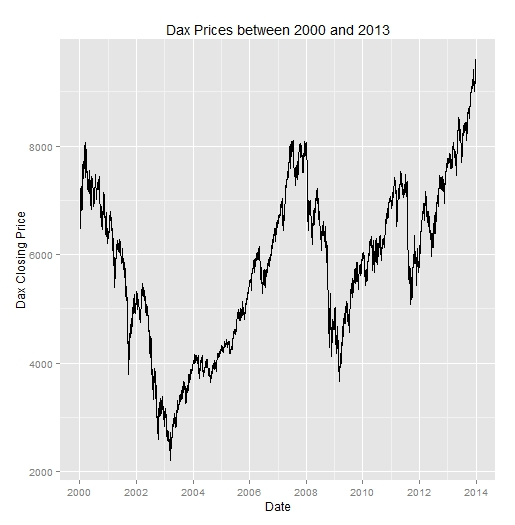
\includegraphics[width=9cm]{chp3_Dax2000_2013}
\caption[Graph of DAX between 2000 and 2013]{Graph of German DAX between 2000 and 2013.}
\label{fig:Dax2000_2013}
\end{figure}

% ------ Graph of Dax 2000 to 2013 --------------
\begin{figure}[tbph]
\centering
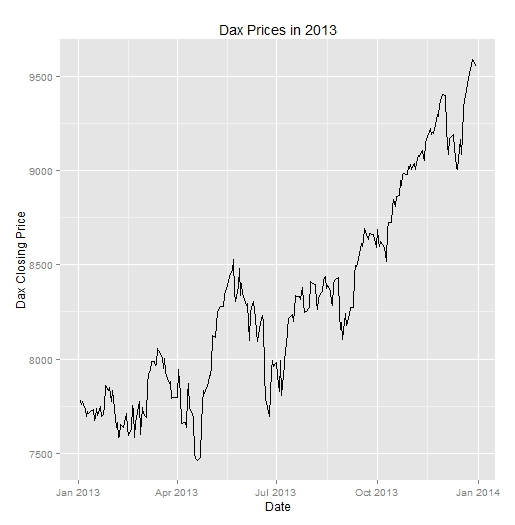
\includegraphics[width=9cm]{chp3_Dax_2013}
\caption[Graph of DAX in 2013]{Graph of German DAX in 2013.}
\label{fig:Dax2013}
\end{figure}

Each data set has a particular set of characteristics and these are important when technical analysis and other analytical techniques are applied to the data set \citep{Chen201466,Matheson2012441}. A variety of these are explored in the following sections. The average amount a market moves is investigated and the term Average True Range is introduced and defined for the data sets. Where the opening and closing prices are in relation to the previous day's high and low values are also considered. Finally, the distance between the day's opening and high prices and opening to low prices are investigated. The relative ratios of these values are important when considering which technical analysis may be best suited to a particular market.

\subsection{Average True Range (ATR)}
\label{chp3:atr}
\cite{wilder1978new} introduced the concept of Average True Range (ATR) as a way to measure a market's volatility or the amount the price is likely to move in any one day. Initially the True Range (TR) is calculated as the maximum of:
\begin{enumerate}
\item the today's high price minus today's low price.
\item the absolute value of the today's high minus the previous day's closing price.
\item the absolute value of the today's low minus the previous day's closing price.
\end{enumerate}
Having calculated the TR, an average of a previous number of days is used to derive the ATR. Typically the TR values from the previous 14 days are used.

Absolute values are used in the calculation of the ATR as we are not concerned with the market direction but rather the the amount the market is likely to move. ATRs are typically quoted as absolute values and as such markets trading at higher prices will have higher ATRs. For example the Japanese Nikkei with a value of 14000 will move more in a day than the French CAC with a value in the 4000's. 

Dividing the ATR by the closing price is a useful way to see how a security's volatility varies over time. Table \ref{tab:atr_dax} shows summary statistics for the ATR and ATR divided by closing price and Figure \ref{fig:Dax_atr} is a graph of how ATR divided by closing price has varied for the DAX between 2000 and 2013. In absolute terms the ATR varied between 36 and 316, however the value of the indice itself varied a lot. Looking at the ATR value divided by the closing period it can be seen that over the period of 2000 to 2014 the mean value is approximately 2. Thus on average the market can be expected to move 2\% of the closing price in any one day. However this value has varied between 0.7\% in periods of low volatility to a value of 6.7\%.

% Table created by stargazer v.4.5.3 by Marek Hlavac, Harvard University. E-mail: hlavac at fas.harvard.edu
% Date and time: Mon, Mar 24, 2014 - 21:57:13
\begin{table}[!htbp] \centering 
  \caption[Average True Range of DAX]{ATR and ATR divided by closing price for the DAX between 2000 and 2013} 
  \label{tab:atr_dax} 
\begin{tabular}{lccccc} 
\toprule
Statistic & N & Mean & St. Dev & Min & Max \\ 
\midrule
ATR & 3,556 & 108.29 & 45.53 & 36.07 & 316.04 \\ 
ATR/Close & 3,556 & 1.995 & 1.065 & 0.700 & 6.740 \\ 
\bottomrule
%\normalsize 
\end{tabular} 
\end{table} 

% ------ Graph of DAX/Closing Price 2000 to 2013 --------------
\begin{figure}[tbph]
\centering
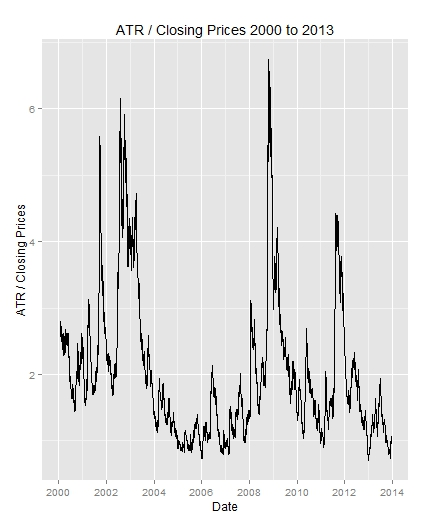
\includegraphics{chp3_Dax_atr}
\caption[ATR of DAX Divided by Closing Price]{ATR of DAX divided by closing price between 2000 and 2013.}
\label{fig:Dax_atr}
\end{figure}

\subsection{Opening Price}
Where a market opens in relation to the previous day's high and low price varies across the data sets. This is important and can influence the technical analysis indicator or trading system to utilise. Table \ref{tab:openprices} lists opening price statistics for a variety of national indices. The table lists the number of times that opening prices are between the previous day's high and low prices. These statistics are useful in characterising a market in terms how they move out of hours and can have an impact when choosing a trading system.

\begin{table}[!htbp] \centering 
  \caption[Opening Prices in relation to previous day's High and Low values]{Opening prices in relation to the previous day's high and low values.} 
  \label{tab:openprices}
\begin{tabular}{lc} 
\toprule 
Market & Opening Price between Previous   \\ 
       &  Day's High and Low (\%) \\
\midrule 
DAX & 75 \\ 
FTSE & 90  \\ 
CAC & 60  \\ 
Dow & 98 \\ 
Nikkei & 53 \\ 
AORD & 79\\ 
\bottomrule 
%\normalsize 
\end{tabular} 
\end{table} 

% Orig table
%\begin{table}[!htbp] \centering 
%  \caption[Opening Prices in relation to previous period.]{Opening prices in relation to the previous day's high and low values a. percentage of times open is between previous high and low b. open price is within a band 10\% below high and above low and c. within a band 30\% below high and above low.} 
%  \label{tab:openprices}
%\begin{tabular}{lccccc} 
%\toprule 
%Market & Open in Prev HL & Open in Prev HL +/-10\% & Open in Prev HL +/-30\%  \\ 
%\midrule 
%DAX & 75\% & 60\% & 29\%  \\ 
%FTSE & 90\% & 70\% & 32\%  \\ 
%CAC & 60\% & 49\% & 25\%  \\ 
%Dow & 98\% & 85\% & 49\%  \\ 
%Nikkei & 53\% & 43\% & 21\%  \\ 
%AORD & 79\% & 64\% & 29\%  \\ 
%\bottomrule 
%%\normalsize 
%\end{tabular} 
%\end{table} 

\subsection{Closing Price}
\label{sec:closing_prices}
In a similar fashion to the opening prices the position of the closing prices in relation to the previous day's high and low price are also of interest. In this case, the percentage of closes outside the previous high/low price may indicate that the market may be a good choice for a breakout type of trading system (see section \ref{sec:chp5:bout_sys} for details of breakout systems). Likewise the opposite situation occurs if a market frequently finishes within the previous day's high and low levels and may be a candidate for a reversal type of system. The statistics for various national indices can be seen in Table \ref{tab:closeHL}. Looking at these figures it would suggest that the Dow with a low ratio of finishing outside the previous period's high low values may be a candidate for a reversal type of system and conversely the Japanese Nikkei has a high percentage value and potentially a candidate for a breakout system.

\begin{table}[!htbp] \centering 
  \caption[Closing Prices in relation to previous day's High and Low values]{Number of occasions when closing prices finished outside the previous day's high or low values.} 
  \label{tab:closeHL}
\begin{tabular}{lc} 
\toprule 
Market & Closing Price outside Previous   \\ 
       &  Day's High and Low (\%) \\
\midrule 
DAX & 56 \\ 
FTSE & 56  \\ 
CAC & 58 \\ 
Dow & 39  \\ 
Nikkei & 63 \\ 
AORD & 60 \\
\bottomrule 
%\normalsize 
\end{tabular} 
\end{table} 

The range from opening price to closing price, either up or down, is of interest. Table \ref{tab:OCrange} lists the minimum and maximum values in this range and Table \ref{tab:OCQuantile} shows the quantiles for this price range.

\begin{table}[!h] \centering 
  \caption[Daily Open to Close Price Range]{Minimum and maximum values for the open to close price range.} 
  \label{tab:OCrange}
\begin{tabular}{lcc} 
\toprule 
Market & Min Value & Max Value  \\ 
\midrule
DAX  & 0 & 508  \\ 
FTSE & 0 & 431  \\ 
CAC  & 0 & 313  \\ 
Dow  & 0 & 950  \\ 
Nikkei & 0 & 1333  \\ 
AORD   & 0 & 347  \\ 
\bottomrule
%\normalsize 
\end{tabular} 
\end{table} 


\begin{table}[!htbp] \centering 
  \caption[Quantiles of the open to close price range]{Quantile values for the open to close price range.} 
  \label{tab:OCQuantile}
\begin{tabular}{lcccc} 
\toprule 
Market & 25\% & 50\% & 75\% & 90\% \\ 
\midrule
DAX  & 16  & 39 & 75 & 508  \\ 
FTSE & 15  & 33 & 63 & 431 \\ 
CAC  & 11  & 26 & 49 & 313 \\ 
Dow  & 27 & 61  & 119 & 950 \\ 
Nikkei & 32  & 71  & 133 & 1333 \\ 
AORD   & 8  & 19  & 36 & 347 \\ 
\bottomrule
%\normalsize 
\end{tabular} 
\end{table} 


%\newcolumntype{d}{D{.}{.}{2.3}}
%\newcolumntype{C}{>{\centering}p}

%\begin{table}[htdp]
%\caption[Closing Prices in relation to previous period.]{Closing prices in relation to the previous day's high and low values.}
%\centering
%\begin{center}
%\begin{tabular}{p{0.7in}ccc}
%\toprule
%\multicolumn{1}{p{0.7in}}{Market} & 
%\multicolumn{1}{C{1.25in}}{Close outside previous HL (\%)} & 
%\multicolumn{1}{C{1.25in}}{Close outside previous HL +/-10\% (\%)} &
%\multicolumn{1}{C{1.25in}}{Close outside previous HL +/-30\% (\%)}\\
%\midrule
%DAX & 56 & 64 & 81  \\ 
%FTSE & 56 & 63 & 81  \\ 
%CAC & 58 & 66 & 83  \\ 
%Dow & 39 & 48 & 72  \\ 
%Nikkei & 63 & 70 & 84  \\ 
%AORD & 60 & 68 & 84  \\ 
%\bottomrule
%\end{tabular}
%\end{center}
%\label{tab:closeHL}
%\end{table}
%
%
%\ctable[
%cap = Closing Prices in relation to previous period,
%caption = Closing prices in relation to the previous day's high and low values
%]
%{lccc }
%{\tnote{Close price is outside of the previous high minus 10\% or the low plus 10\%}
%\tnote[b]{Close price is outside of the previous high minus 30\% or the low plus 30\%}}
%{
%\FL
%Market &  Close Outside   &  Outside Previous      & Outside Previous \\
%DAX    & Previous HL      &  HL +/- 10\% \tmark   &  HL +/- 30\% \tmark[b]         \ML
%DAX & 56 & 64 & 81  \\ 
%FTSE & 56 & 63 & 81  \\ 
%CAC & 58 & 66 & 83  \\ 
%Dow & 39 & 48 & 72  \\ 
%Nikkei & 63 & 70 & 84  \\ 
%AORD & 60 & 68 & 84  \LL
%}


%\begin{table}[!htbp] \centering 
%  \caption[Closing Prices in relation to previous period.]{Closing prices in relation to the previous day's high and low values a. percentage of times close is greater than previous high or lower than previous low b. open price is greater than a band 10\% below high and above low and c. greater than a band 30\% below high and or above the low.} 
%  \label{tab:closeHL2}
%\begin{tabular}{lccccc} 
%\toprule 
%Market & Close out Prev HL & Close out Prev HL(1090) & Close out Prev HL(3070)  \\ 
%\midrule
%DAX & 56\% & 64\% & 81\%  \\ 
%FTSE & 56\% & 63\% & 81\%  \\ 
%CAC & 58\% & 66\% & 83\%  \\ 
%Dow & 39\% & 48\% & 72\%  \\ 
%Nikkei & 63\% & 70\% & 84\%  \\ 
%AORD & 60\% & 68\% & 84\%  \\ 
%{\footnotesize a bit of text} \\
%\bottomrule
%%\normalsize 
%\end{tabular} 
%\end{table} 


\subsection{High/Low Price}
Table \ref{tab:highlow} shows the percentage of times that either today's high price crosses yesterday's high or today's low prices dips below yesterday's low value. The final closing price may be between yesterday's high and low or outside of it. The second column of Table \ref{tab:highlow} is the number of times when today's values crossed both the previous low and the previous high in the same day. This is also known as an Engulfing Candlestick (see section \ref{sec:eng_cand}). In all the indices the previous day's high or low value is reached the following day in a large number of instances, in the case of the Nikkei 90\% of the time. Conversely, the likelihood of both the previous day's high and low values being touched are low, only 5\% of occasions in the Australian AORD. 

\begin{table}[!htbp] \centering 
  \caption[Today's H/L Prices in relation to previous day's HL]{Number of occasions when today's high or low prices crossed the previous day's high or low values.} 
  \label{tab:highlow}
\begin{tabular}{lcc } 
\toprule 
Market & Crosses either previous    & Crosses both the previous \\ 
       & day's High or Low (\%)     &  day's High and Low (\%)       \\
\midrule 
DAX  & 89  & 9  \\ 
FTSE & 87  & 8  \\ 
CAC  & 90  & 10 \\ 
Dow  & 88  & 9  \\ 
Nikkei & 90 & 8 \\ 
AORD   & 86 & 5 \\
\bottomrule 
%\normalsize 
\end{tabular} 
\end{table} 

%\begin{table}[!htbp] \centering 
%  \caption[Today's High/Low Prices in relation to the previous period.]{Today's High/Low prices in relation to the previous day's high and low values a. percentage of times high/low is greater than previous high or lower than previous low b. open price is greater than a band 10\% below high and above low and c. greater than a band 30\% below high and or above the low.} 
%  \label{tab:highlow}
%\begin{tabular}{lcccc} 
%\toprule
%Market & \parbox[c]{2cm}{HL crosses Prev HL} & \parbox[c]{3cm}{HL crosses \\both Prev HL} & \parbox[c]{3cm}{HL crosses\\ Prev HL(1090)} & \parbox[c]{3cm}{HL crosses both Prev HL(1090)}  \\ 
%\midrule
%DAX  & 89\% & 9\%  & 95\% & 16\% \\ 
%FTSE & 87\% & 8\%  & 95\% & 15\% \\ 
%CAC  & 90\% & 10\% & 95\% & 16\% \\ 
%Dow  & 88\% & 9\%  & 97\% & 21\% \\ 
%Nikkei & 90\% & 8\%  & 95\% & 12\% \\ 
%AORD   & 86\% & 5\%  & 94\% & 10\% \\ 
%\bottomrule
%\normalsize 
%\end{tabular} 
%\end{table} 

\subsection{OH/OL Price Fluctuations}
\label{sec:ohol:fluctuation}
The movements in prices between the open and high (OH) and open to low (OL) are interesting and can have an influence on any trading systems developed. On any given day prices open, move to their lowest point, move to their highest point and then close (not in any particular order). From the OHLC data used in this study the order of these events can not be determined or even the number of times in a day these price points are reached. 

In this section we are concerned with the relative sizes of these two price movements, the day's high price minus the opening price (OH) and the opening price minus the low price (OL), one of which is usually greater than the other. We will define the daily \textquotedblleft minor" price fluctuation as the smaller of the two price movements. Likewise we will define the larger value as the \textquotedblleft major" price fluctuation.

Considering the minor price fluctuation, the range of values encountered in the indice markets under study can be seen in Table \ref{tab:minorOH}. In all cases the minimum value is zero, in other words the market opening price and either the day's high or low price were the same, the market didn't dip below or above this level. The second column in Table \ref{tab:minorOH} is the maximum value. In the case of the German DAX, there was a day when the market moved 189 points away from its opening price but also moved further in the opposite direction away from the opening price. Clearly this was a highly volatile day on the German markets.

\begin{table}[!h] \centering 
  \caption[Minor daily price fluctuation]{Minimum and maximum values for the smaller of the daily OH or OL price movement - the \textquotedblleft minor" move.} 
  \label{tab:minorOH}
\begin{tabular}{lcc} 
\toprule 
Market & Min Value & Max Value  \\ 
\midrule
DAX  & 0 & 189  \\ 
FTSE & 0 & 186  \\ 
CAC  & 0 & 134  \\ 
Dow  & 0 & 379  \\ 
Nikkei & 0 & 310  \\ 
AORD   & 0 & 114  \\ 
\bottomrule
%\normalsize 
\end{tabular} 
\end{table} 

The quantiles of the minor price movements can be seen in Table \ref{tab:minorOHQ}. The 90\% quantile is the level at which 90\% of the time the minor move is less than this level.  This value may be important to know and understand when considering breakout type of systems (see section \ref{sec:bout}).  Looking at the value of the DAX we can see that the 90\% quantile level occurs at 46, which indicates that if the market has moved to this level it is unlikely to be the day's minor move (whose level 90\% of the time is below this).  Perhaps a breakout type of system may be profitable at this point, as once the market has moved this far it is usually a major move and may be expected to continue further in the same direction.

\begin{table}[!htbp] \centering 
  \caption[Quantiles of Minor daily price fluctuation.]{Quantile values for the smaller of the days OH or OL price movement - the \textquotedblleft minor" move.} 
  \label{tab:minorOHQ}
\begin{tabular}{lcccc} 
\toprule 
Market & 25\% & 50\% & 75\% & 90\% \\ 
\midrule
DAX  & 5  & 15 & 29 & 46  \\ 
FTSE & 0  & 7 & 20 & 33 \\ 
CAC  & 4  & 11 & 19 & 31 \\ 
Dow  & 12 & 43  & 75 & 113 \\ 
Nikkei & 5  & 21  & 43 & 72 \\ 
AORD   & 0  & 1  & 7 & 13\\ 
\bottomrule
%\normalsize 
\end{tabular} 
\end{table} 

In contrast to the minor daily price fluctuation, the \textquotedblleft major" price fluctuation is defined as the largest of the OH or OL values.  The range of values encountered in this price fluctuation in the indice markets can be seen in Table \ref{tab:majorOH} and the quantiles of the major price movements can be seen in Table \ref{tab:majorOHQ}. Considering the DAX once more, it can be seen that the 25\% quantile is approximately equal to the 90\% quantile of the minor fluctuation. Thus if the DAX moves approximately 50 points away from the opening it is unlikely to be the smaller of the price movements and much more likely to be part of the larger movement. Knowledge of the minor and major price fluctuations may be useful in developing trading systems. 

\begin{table}[!h] \centering 
  \caption[Major daily price fluctuation.]{Minimum and maximum values for the larger of the days OH or OL price movement - the \textquotedblleft major" daily price fluctuation.} 
  \label{tab:majorOH}
\begin{tabular}{lcc} 
\toprule 
Market & Min Value & Max Value  \\ 
\midrule
DAX  & 0 & 530  \\ 
FTSE & 0 & 471  \\ 
CAC  & 0 & 359  \\ 
Dow  & 0 & 992  \\ 
Nikkei & 0 & 1737  \\ 
AORD   & 0 & 347 \\ 
\bottomrule
%\normalsize 
\end{tabular} 
\end{table} 

\begin{table}[!htbp] \centering 
  \caption[Quantiles of Major daily price fluctuation.]{Quantile levels for the larger of the day's OH or OL price movement - the \textquotedblleft major" daily price fluctuation.} 
  \label{tab:majorOHQ}
\begin{tabular}{lccc} 
\toprule 
Market & 25\% & 50\% & 75\% \\ 
\midrule
DAX  & 43  & 69 & 106  \\ 
FTSE & 37  & 56 & 86  \\ 
CAC  & 30  & 45 & 69  \\ 
Dow  & 92 & 131  & 190  \\ 
Nikkei & 76  & 118  & 184  \\ 
AORD   & 18  & 30  & 48 \\ 
\bottomrule
%\normalsize 
\end{tabular} 
\end{table} 

A final consideration in this section is the range of the open to close prices detailed in section \ref{sec:closing_prices}. Again considering the German DAX it can be seen that the 50\% quantile value is 39, as shown in Table \ref{tab:OCQuantile}, which is below the 90\% minor fluctuation level.

%\begin{table}[!htbp] \centering 
%  \caption[Quantiles of the open to close price range.]{Quantile values for the open to close price range.} 
%  \label{tab:OCQuantile2}
%\begin{tabular}{lcccc} 
%\toprule 
%Market & 25\% & 50\% & 75\% & 90\% \\ 
%\midrule
%Dax  & 16  & 39 & 75 & 508  \\ 
%FTSE & 15  & 33 & 63 & 431 \\ 
%CAC  & 11  & 26 & 49 & 313 \\ 
%Dow  & 27 & 61  & 119 & 950 \\ 
%Nikkei & 32  & 71  & 133 & 1333 \\ 
%AORD   & 8  & 19  & 36 & 347 \\ 
%\bottomrule
%%\normalsize 
%\end{tabular} 
%\end{table} 

\section{Software Tools}

\subsection{R and R Studio}
Experimental results and graphs were produced with the open source programming language R version 3.0.2. For help in the creation and organisation of the R code for this thesis the open-source development environment R Studio version 0.98.490 was used extensively. The following packages were immensely helpful in the preparation of this thesis:
\begin{itemize}
\item TTR - provided technical analysis functions
\item xts - irregularly spaced time series
\item forecast - time series forecasting
\item candlestick - Japanese candlestick patterns
\end{itemize}

\subsection{Rapid Miner}
Rapid Miner version 5.3, a market leading open-source data mining and predictive analytic platform, was used for building hybrid ARIMA models. The base system and time series plug-ins were used.

\section{Methodology}
The aim of this study was to predict market movement, not in terms of absolute values but more in terms of general direction. The trading algorithms developed in this study were based around a daily time period. The data used was daily data containing open, high, low and closing prices. The trading algorithms developed typically opened a trade at the day's opening price and closed them at the day's closing prices. There are some deviations from this, for example trades are closed at some pre-defined point in the event of a stop loss being entered or trades running from close to close, and these are detailed in the text at the appropriate place. 

Prior to passing the data sets to the trading algorithms they were subjected to either technical or time series analysis. Typically technical analysis results in the generation of a value (for example a moving average or stochastic value) which is considered meaningful in the future prediction of the financial market. 
The forecasts produced from the technical analysis and time series models were consumed by the trading algorithms and used to decide in which direction the daily trade would be made, i.e. would the market rise or fall.

The success or failure of any particular method was determined by the number of points gained or lost in these trading algorithms. In turn these points can be considered money and the net number of points can represent a profit or loss (PL). The results presented in Chapters \ref{Chapter4} and \ref{Chapter5} report either the total PL of a system or the average PL per trade. The latter value is probably most useful when it comes to comparing systems that don't enter trades every day, for example when one uses candlestick patterns which only occur very infrequently. Also the direction of trade is also a consideration. Results are separated into long (a buy is made in the expectation of the market rising) or short (a sell is made in the expectation of the market falling).

% Chapter 4

\chapter{Technical Analysis} % Main chapter title
 
\label{Chapter4} % For referencing the chapter elsewhere, use \ref{Chapter5} 

\lhead{Chapter 4. \emph{Technical Analysis}} % This is for the header on each page - perhaps a shortened title

%---------------------------------------------------------------------------------------
\section{Introduction}
This chapter investigates whether technical analysis can provide a positive expectanacy for financial traders. A variety of technical analysis indicators are employed including MACD, Aroon, Stochastics Oscillator and Rate of Change (ROC) indicator. The experimental reslts from using these indicators are presented in groupings based on the general category of indicator such as trend identification or market reversal indicators. Some technical indicators have a role to play in more than one area, such as MACD, and as such the categorisation is quite general.

The effectiveness of a particular indicator or system is measured in terms of \textquotedblleft points" gained, which is also referred to as \textquotedblleft PL" (which stands for to profit and loss). The results presented in this chapter are mainly based around systems in which a trade is opened and closed each day, producing a daily PL either positive or negative. The sum of all the individual days produces the total system PL and these values are reported in the results tables. For example, if the market moved from 6000 to 6200 in any one day a PL of either 200 (6200 - 6000) or -200 (6000 - 6200) depending upon which way the trade was placed, would be added to the overall system results. 

In addition, the results are presented such that returns from \textquotedblleft going Long" (expecting the market to rise) are presented seperately from the opposite scenario of \textquotedblleft going Short". This is because  market behaviour is often different while it is rising than it is while falling and systems may be more adept at predicitng price movements in one of the directions. Further, transactions costs are not taken into account in the results and these would typically be 1 point per trade for the European markets, 2 points for the Dow and 10 for the Nikkei.  Thus if a system made a PL of 1000 but it required 2000 trades at 2 points per trade, in reality the system would have lost money. 

The results presented in this chapter and the following one are based around trading systems. Essentially the methodology concerned, technical analysis in this chapter and time series analysis in the next, attempt to predict future market direction. The values from the various indicators and forecast techniques are fed into a variety of trading algorithms which use the forecast information to decide whether to make long (expect the market to rise) or short (expect the market to fall) trades. For consistency the algorithms all return the same data object containing the following results:

\begin{enumerate}
\item Mkt - the name of the financial market such as Dax, FTSE etc.
\item S Loss - the value of any stop loss applied
\item LongPL - the profit or loss generated from just the \textquotedblleft Long" trades.
\item ShortPL - the profit or loss generated from just the \textquotedblleft Short" trades.
\item L Win \% - the percentage of time the Long trades win.
\item L Trades - the number of Long trades executed.
\item Av L PL - the average profit or loss generated from each Long trade.
\item S Win \% - the percentage of time the Short trades win.
\item S Trades - the number of Short trades executed.
\item Av S PL - the average profit or loss generated from each Short trade.
\item misc - miscellaneous information such as the SMA used in the algorithm.
\end{enumerate}

The results from Long and Short trades in particular trading algorithm are considered separately as frequently markets behave differently as they move up as opposed to as they fall. Further, the percentage of times the algorithm results in winning trades, the number of trades and the average profit or loss (PL) for each trade is reported for both Long and Short trades. The average PL is primarily reported in the following results tables because this allows comparisons between systems that generate a lot of trades with those such as the algorithms based on candlestick patterns that results in only a small number of trades. 

% --------------------------------------------------------------------------------------
\section{Baseline Systems - Naive Methods}
Initially two very simple ideas were explored in order for the results to be used as baselines against which the technical indicators explored in the rest of the chapter can be compared. There is an expectation that the use of technical indicators will produce systems that provide much better results than these two so-called naive systems.

The first system simply uses the idea that markets tend to increase in value over time. The algorithm applies a naive approach and simply enters a trade each day expecting the market to rise. The well-known method of "Buy and Hold" applies the same principles. The total PL of the resulting system is the the sum of all the daily close minus open prices. This approach has been named a \textquotedblleft Naive Long System".

The second approach is equally simplistic, and again is based around opening and closing a trade each day. A notable difference from the first naive system is that the algorithm can result in either a buy or a sell (expecting the market to decline in value) occurring. If a market increased in price the previous day the algorithm \textquotedblleft reverses" it and expects the market to fall today. Likewise if the market had fallen the previous day the system buys the market today. This idea has been named the \textquotedblleft Naive Reversing System".

%-----------------------------------------------------------------
% ---------------------------  Naive Long ------------------------
\subsection{Naive Long System}
The results of the naive long system can be seen in Table \ref{tab:nlng_results}. The R code for the algorithm which generates the results shown in Table \ref{tab:nlng_results} can be seen in Appendix \ref{AppendixA} section \ref{appA:NaiveLong}. For comparison purposes, the opening prices of the indices in January 2000 along with the closing prices in 2013 can be seen in Table \ref{tab:ind_start_stop}. In this period three of them increased in value (Dax, Dow and AORD) and three decreased (FTSE, CAC and Nikkei).

Interestingly, the PL produced from the Naive Long System doesn't match the price differentials seen in Table \ref{tab:ind_start_stop}.  The German Dax indice produced a marked loss in the naive system even though it actually increased 37\% during this period. The Japanese Nikkei declined by over 2600 points in this period, whereas the system reported a loss of over 18000 points in the same period. On the other hand the US Dow increased by around 5000 points during the period of the study but the trading algorithm produced a positive result of almost 10000. These discrepancies can be explained by the fact that the system was using prices from the market's opening to closing times, which represents approximately  eight hours of trading between 8am and 4pm local time. These price movements don't account for the rest of the hours, the so-called out of market hours, when the market prices also change. Clearly the markets show different characteristics in the amount they move during market hours compared to out of market hours. The Nikkei, Dax and CAC have a tendency to fall during market hours and rise during out of market hours. The opposite situation occurs for the Dow.

% Table
% latex table generated in R 3.1.0 by xtable 1.7-3 package
% Sat May 24 09:31:35 2014
\begin{table}[ht]
\centering
\caption[Naive Long System]{Naive Long System. A very simple system in which the algorithm assumes the market will rise and enters a long trade each day.} 
\label{tab:nlng_results}
\begin{tabular}{lccc}
  \toprule Mkt & LongPL & L Win \% & L Trades \\ 
  \midrule Dax & -1714 & 52 & 3528 \\ 
  CAC & -6725 & 50 & 3586 \\ 
  F100 & 149 & 51 & 3532 \\ 
  Dow & 9816 & 53 & 3521 \\ 
  Nik & -18125 & 49 & 3438 \\ 
  Oz & 972 & 52 & 3548 \\ 
   \bottomrule \end{tabular}
\end{table}


% ---------- Table
\begin{table}[!htbp] \centering  
\caption[Indice Prices in 2000 and 2013.]{Prices of six national indices in January 2000 and December 2013.}
\label{tab:ind_start_stop}
\begin{tabular}{lcccc}
\toprule
Date & Start 2000 & End 2013 & Difference & \% Change  \\
\midrule
Dax & 6961 & 9552   & +2591 & +37 \\
CAC & 6024 & 4250   & -1774 & -29 \\
FTSE & 6930 & 6749  & -181  & +-3 \\
Dow & 11501 & 16576 & +5075 & +44 \\
Nik & 18937 & 16291 & -2646 & -14 \\
AORD & 3152 & 5353  & +2201 & +70 \\
\bottomrule
\end{tabular}
\end{table}

Altering the algorithm slightly so that a trade represents the difference between the previous closing price and today's closing price affects the results markedly. A full 24 hour period is now accounted for and the system reflects the overall market movement during this period. These results can be seen in Table \ref{tab:nlng_results_2} and the amended R code can be seen in Appendix \ref{AppendixA} section \ref{appA:NaiveLong_2}.

% Table
% latex table generated in R 3.1.0 by xtable 1.7-3 package
% Tue Aug 19 13:19:47 2014
\begin{table}[ht]
\centering
\caption[Results from the Naive Long System trading close to close]{Naive Long System changed such that the trading period is the previous close price minus today's close.} 
\label{tab:nlng_results_2}
\begin{tabular}{lccc}
  \toprule Mkt & LongPL & L Win \% & Av L PL \\ 
  \midrule DAX & 2649 & 53 & 1 \\ 
  CAC & -1667 & 51 & 0 \\ 
  FTSE & 86 & 51 & 0 \\ 
  Dow & 5219 & 53 & 1 \\ 
  Nikkei & -2712 & 51 & -1 \\ 
  AORD & 2229 & 53 & 1 \\ 
   \bottomrule \end{tabular}
\end{table}


\subsection{Naive Reversing System}
\label{sec:naive:rev}
The second naive method is to reverse the previous day's movement. For example, if the market closed up the previous day the algorithm follows this by trading short for the current day (the R code for this algorithm can be see in Appendix \ref{AppendixA} section \ref{appA:NaiveFollowPrev}) . The results from this system can be seen in Table \ref{tab:ntfresults}. 

% \label{tab:ntfresults}
% latex table generated in R 3.1.0 by xtable 1.7-3 package
% Mon Jun 02 13:01:39 2014
\begin{table}[ht]
\centering
\caption[Naive Following System.]{Naive system which repeats the previous day's trade direction.} 
\label{tab:ntfresults}
\begin{tabular}{lcccccc}
  \toprule Mkt & LongPL & ShortPL & L Win \% & L Trades & S Win \% & S Trades \\ 
  \midrule Dax & -3131 & -947 & 51 & 1826 & 47 & 1672 \\ 
  CAC & -7810 & -940 & 47 & 1786 & 47 & 1798 \\ 
  F100 & -4115 & -4284 & 50 & 1815 & 47 & 1712 \\ 
  Dow & -6047 & -15799 & 51 & 1870 & 44 & 1646 \\ 
  Nik & -20486 & -2324 & 46 & 1665 & 49 & 1769 \\ 
  Oz & -237 & -1264 & 52 & 1851 & 47 & 1682 \\ 
   \bottomrule \end{tabular}
\end{table}


For all the markets tested, this second naive system produces positive results especially for the Nikkei and CAC trading short and the Dow trading long. These results demonstrate that markets have a tendency to reverse direction each day, they move up one day then down the next. This behaviour is also observed in trending markets, and market \textquotedblleft pull-backs" are a well-known phenomena.

\subsection{Summary of Naive Baseline Systems}
Of the two naive systems tested, the \textquotedblleft reversing" methodology produces the best results in terms of profit and loss by quite a margin. Thus the results from the \textquotedblleft Naive Reversing System" will be used to compare the performance of technical indicators being tested in the following sections.

\section{Trend Detection Indicators}
\label{sec:trend}

One of the most widely used phrases in financial trading is \textquotedblleft the trend is your friend". Thus, most market participants are interested in identifying the start of trends, their direction and strength. In this section a variety of technical indicators that purport to assist in this important task are tested. 

\subsection{Simple Moving Average (SMA) System}
\label{sec:Chp4a:sma}
One of the most popular and widely utilised technical indicators is the simple moving average (as detailed in Chapter \ref{Chapter2} section \ref{sec:chp2_sma}). The effectiveness of SMA as an aid to predicting future market movements has been widely debated, with views mixed. A system based on simple moving averages is presented here, and the R code used to generate the results can be seen in Appendix \ref{AppendixA} section \ref{appA:SMA_sys}. The algorithm trades daily, opening and closing a trade each day.  If the market opens above the SMA the algorithm trades long and trades short when the market opens below the SMA.

Table \ref{tab:sma_results} lists the results from passing a variety of national index data sets (see Chapter \ref{Chapter3} for details) to the algorithm. For each indice the algorithm is run with values of 5, 25, 50, 100 and 200 for the SMA period. In general the results are poor, especially after consideration is given to any transaction costs. The CAC and Nikkei produce negative results for long trades, the FTSE negative results across the board, and the Dow negative returns on the short side.

% latex table generated in R 3.1.0 by xtable 1.7-3 package
% Mon Jun 23 18:28:29 2014
\begin{table}[ht]
\centering
\caption[Results from a system based on SMA]{Results from a system based on SMA.} 
\label{tab:sma_results}
\begin{tabular}{lccccccc}
  \toprule Mkt & LongPL & ShortPL & L Win \% & Av L PL & S Win \% & Av S PL & SMA \\ 
  \midrule Dax & 2113 & 3278 & 54 & 1 & 50 & 2 & 0 \\ 
  Dax & 1367 & 3427 & 54 & 1 & 50 & 2 & 0 \\ 
  Dax & 779 & 3447 & 54 & 0 & 51 & 3 & 0 \\ 
  Dax & 714 & 2339 & 54 & 0 & 51 & 2 & 0 \\ 
  Dax & 3401 & 4416 & 55 & 2 & 52 & 4 & 0 \\ 
  CAC & -3952 & 2338 & 49 & -2 & 49 & 1 & 0 \\ 
  CAC & -5058 & 1615 & 49 & -2 & 49 & 1 & 0 \\ 
  CAC & -5323 & 1029 & 49 & -3 & 49 & 1 & 0 \\ 
  CAC & -2363 & 3188 & 50 & -1 & 50 & 2 & 0 \\ 
  CAC & -1219 & 3923 & 50 & -1 & 50 & 3 & 0 \\ 
  FTSE & -4724 & -5331 & 49 & -2 & 46 & -3 & 0 \\ 
  FTSE & -1013 & -1940 & 51 & 0 & 47 & -1 & 0 \\ 
  FTSE & -2226 & -2769 & 50 & -1 & 47 & -2 & 0 \\ 
  FTSE & -889 & -1692 & 51 & 0 & 48 & -1 & 0 \\ 
  FTSE & -158 & -835 & 52 & 0 & 49 & -1 & 0 \\ 
  Dow & 408 & -9630 & 52 & 0 & 46 & -6 & 0 \\ 
  Dow & 1138 & -9204 & 53 & 1 & 46 & -7 & 0 \\ 
  Dow & 5478 & -5876 & 53 & 3 & 47 & -4 & 0 \\ 
  Dow & 2576 & -8220 & 53 & 1 & 47 & -6 & 0 \\ 
  Dow & 6378 & -4567 & 54 & 3 & 48 & -4 & 0 \\ 
  Nikkei & 3078 & 20401 & 51 & 2 & 54 & 13 & 0 \\ 
  Nikkei & -7878 & 10770 & 48 & -4 & 52 & 7 & 0 \\ 
  Nikkei & -6054 & 11408 & 49 & -4 & 52 & 7 & 0 \\ 
  Nikkei & -6235 & 8381 & 49 & -4 & 52 & 5 & 0 \\ 
  Nikkei & -5928 & 6836 & 49 & -4 & 52 & 4 & 0 \\ 
  AORD & 5009 & 3929 & 55 & 3 & 51 & 3 & 0 \\ 
  AORD & 3701 & 2674 & 54 & 2 & 50 & 2 & 0 \\ 
  AORD & 2804 & 1864 & 54 & 1 & 50 & 1 & 0 \\ 
  AORD & 2688 & 1521 & 54 & 1 & 50 & 1 & 0 \\ 
  AORD & 2574 & 1616 & 54 & 1 & 51 & 2 & 0 \\ 
   \bottomrule \end{tabular}
\end{table}



One aspect of a trading system of this nature worth considering is the risk / reward profile. As written in its current form the SMA algorithm has an unlimited profit potential (trades are left to run until the end of the day) and an unlimited potential loss for the same reason. Often traders employ what is known as a \textquotedblleft stop loss". This is a level in the market that if reached during a trade will cause the trade to close. The risk is now therefore reduced to this value while the profit is still potentially uncapped. Table \ref{tab:sma_results_Sloss} lists the results of using a stop loss with the SMA system.

The logic of the stop loss was coded as follows. Considering a long trade (the opposite holds true for trading short), where there is an expectation that the market to rise, a the stop loss would be triggered if the market fell to a certain  level. Thus in the algorithm for a long trade the distance from the opening price to the low is calculated and this is compared to the stop loss value. If the open to low value exceeds the stop loss value the PL for this particular trade is set at the stop loss value, for example a loss of 100 points. One point of note is the fact that after hitting this low level the market may well recover and move upwards as originally expected. In many cases a trade that ultimately would have been profitable may be \textquotedblleft stopped out" by the natural wax and wane of the markets. Therefore the impact of a stop loss is the balance between lost good trades and the reduction in the lost PL from losing trades. The size of the stop loss determines the impact of the two competing situations.

\begin{figure}[tbph]
\centering
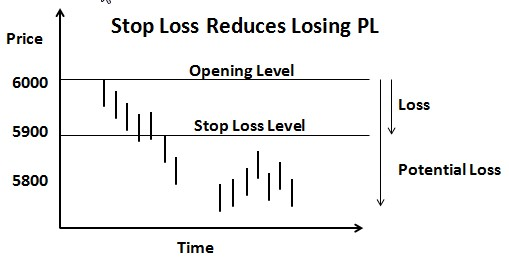
\includegraphics[width=9cm]{chp5b_StopLoss1}
\caption[ Stop Loss.]{Situation in which using a Stop Loss is beneficial, with a losing PL being reduced..}
\label{fig:chp5:sloss1}
\end{figure}

\begin{figure}[tbph]
\centering
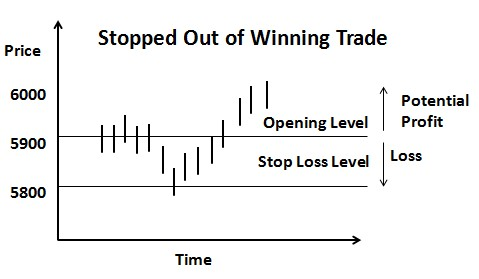
\includegraphics[width=9cm]{chp5b_StopLoss2}
\caption[ Stop Loss.]{Situation in which using a Stop Loss is detrimental, being \textquotedblleft Stopped Out" of an ultimately winning trade.}
\label{fig:chp5:sloss2}
\end{figure}


%\begin{figure}[tbph]
%\centering
%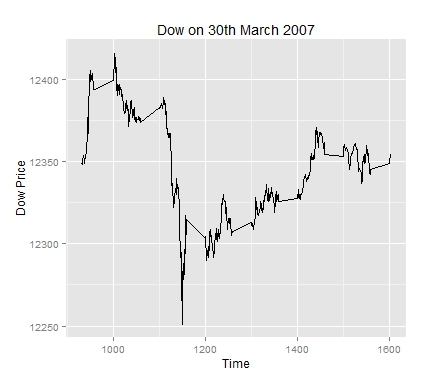
\includegraphics[width=9cm]{chp5b_SLoss_new}
%\caption[ Stop Loss.]{Being Stopped out.}
%\label{fig:chp5:sloss_new}
%\end{figure}


Figure \ref{fig:chp5:sloss1} shows the situation in which a stop loss is benefiical. The potential large loss is reduced to the value of the stop loss value. Figure \ref{fig:chp5:sloss2} illustrates the alternative scenario of being \textquotedblleft Stopped Out" of an ultimately winning trade, an undesirable outcome. It is the ratio of these scenarios that ultimately determines whether using a stop loss is a sound strategy.

% latex table generated in R 3.1.0 by xtable 1.7-3 package
% Wed Jul 09 19:03:39 2014
\begin{table}[ht]
\centering
\caption[Results from a system based on SMA with stop loss]{Results from a system based on SMA with stop loss.} 
\label{tab:sma_results_Sloss}
\begin{tabular}{lcccccccc}
  \toprule Mkt & S Loss & LongPL & ShortPL & L Win \% & L Trades & S Win \% & S Trades & SMA \\ 
  \midrule Dax & -50 & 3652 & 6618 & 51 & 2070 & 42 & 1360 & 0 \\ 
  Dax & -100 & 1392 & 5272 & 54 & 2070 & 50 & 1360 & 0 \\ 
  CAC & -50 & -172 & 5178 & 50 & 2012 & 47 & 1475 & 0 \\ 
  CAC & -100 & -1822 & 4658 & 50 & 2012 & 50 & 1475 & 0 \\ 
  FTSE & -50 & 1114 & 6303 & 50 & 2044 & 43 & 1389 & 0 \\ 
  FTSE & -100 & -885 & 1892 & 51 & 2044 & 47 & 1389 & 0 \\ 
  Dow & -50 & -18212 & -8229 & 32 & 2125 & 22 & 1297 & 0 \\ 
  Dow & -100 & -11771 & -14696 & 49 & 2125 & 36 & 1297 & 0 \\ 
  Nikkei & -50 & 8258 & 33882 & 38 & 1643 & 39 & 1696 & 0 \\ 
  Nikkei & -100 & 2550 & 25582 & 47 & 1643 & 48 & 1696 & 0 \\ 
  AORD & -50 & 4008 & 3730 & 54 & 2230 & 49 & 1219 & 0 \\ 
  AORD & -100 & 2881 & 2149 & 54 & 2230 & 50 & 1219 & 0 \\ 
   \bottomrule \end{tabular}
\end{table}


Comparing Tables \ref{tab:sma_results} and \ref{tab:sma_results_Sloss}
it can be seen that applying the stop loss has been on the whole beneficial to the results obtained, with the exception of those from the Dow which were markedly negatively impacted. Essentially losing trades have been truncated while winning trades have been left to develop. One question that needs to be addressed is what value is appropriate for a stop loss. If the value is large the benefits of cutting losses is lost, whereas if it is too small a large number of trades will be \textquotedblleft stopped out". Many traders use a value based on the Average True Range (see Chapter \ref{Chapter3} section \ref{chp3:atr} for details) as this allows for the volatility of a particular market.

\subsection{Moving Average Convergence/Divergence (MACD)}

Moving Average Convergence/Divergence (MACD) is a trend following indicator, developed by \cite{appel2005technical}, that is formed from the relationship of two moving averages, see Appendix \ref{AppendixB} section \ref{appB:MACD} for more details. The value of MACD itself is the difference between two exponential moving averages (EMA), a \textquotedblleft slower" e.g. 26 day value and a \textquotedblleft faster" e.g. 12 day value. In addition an EMA of the MACD value is calculated, which is set to 9 days in the following algorithm, which acts as a \textquotedblleft signal" line.
 
The MACD is generally used two ways. Firstly, it can be used to derive the general trend of the security so that the market participant can trade with the trend. Secondly, it can be employed to identify periods when the market is \textquotedblleft over-bought" or \textquotedblleft over-sold" and can be expected to reverse direction \citep{MACD2}.

In order to identify the trend of a market using the MACD indicator, the relative values of the MACD itself and the signal line are used. If the value of the MACD exceeds the signal it is considered \textquotedblleft bullish" and the market is expected to rise in price. Similarly in the opposite situation where the value of the signal is greater than the MACD the trend of the market is expected to be down. 

Table \ref{tab:mac_trend_results} lists the results of using the MACD indicator in just such a way. The MACD value itself is generated using the EMA of the opening prices with values of 26 and 12 for the slow and long averages and a value of 9 days for the indicator line. 

The trading algorithm splits the results into two values, days when the system expected the market to rise and days when a market decline were predicted (see Appendix \ref{AppendixA} section \ref{appA:macd_xo} for details of the R code used and Appendix \ref{AppendixB} section \ref{appB:MACD} for background information on the MACD indicator). At the start of each day if the MACD value exceeds the signal line the algorithm adds the value of the close price minus the opening price to the \textquotedblleft Long PL" running total. Likewise in the opposite situation with the signal line greater than the MACD, the value of the open price minus the close price is added to the \textquotedblleft Short PL". Table \ref{tab:mac_trend_results} lists the results of the algorithm run against a variety of national indices.

% latex table generated in R 3.1.0 by xtable 1.7-3 package
% Mon Aug 11 19:25:42 2014
\begin{table}[ht]
\centering
\caption[Results from a system using MACD as a trend indicator]{Results from a system using MACD as a trend indicator.} 
\label{tab:mac_trend_results}
\begin{tabular}{lcccccc}
  \toprule Mkt & LongPL & ShortPL & L Win \% & Av L PL & S Win \% & Av S PL \\ 
  \midrule DAX & -791 & 1424 & 53 & 0 & 48 & 1 \\ 
  CAC & -4153 & 2188 & 49 & -2 & 49 & 1 \\ 
  FTSE & 63 & -839 & 51 & 0 & 48 & 0 \\ 
  Dow & 5592 & -5190 & 53 & 3 & 46 & -3 \\ 
  Nikkei & -4078 & 14064 & 49 & -2 & 52 & 8 \\ 
  AORD & 2563 & 1569 & 54 & 1 & 49 & 1 \\ 
   \bottomrule \end{tabular}
\end{table}



\subsection{Aroon Indicator}
Developed by Tushar Chande in 1995, the Aroon indicator was designed to identify trending markets \citep{aroon_stockcharts}. The word aroon means \textquotedblleft dawn's early light" in Sanskrit and this indicator tries to pin point the dawning of a new trend.  Essentially it is a measure of the time since the occurrence of a high/low price in a particular period. Further details can be seen in Appendix \ref{AppendixB} section \ref{appB:aroon}.

% latex table generated in R 3.1.0 by xtable 1.7-3 package
% Mon Aug 11 19:25:43 2014
\begin{table}[ht]
\centering
\caption[Results from a system based on the Aroon indicator]{Results from a system based on the Aroon indicator.} 
\label{tab:aroon_results}
\begin{tabular}{lcccccc}
  \toprule Mkt & LongPL & ShortPL & L Win \% & Av L PL & S Win \% & Av S PL \\ 
  \midrule DAX & 5308 & 5257 & 56 & 3 & 51 & 4 \\ 
  CAC & -1638 & 4919 & 50 & -1 & 52 & 4 \\ 
  FTSE & 3042 & 5715 & 52 & 2 & 51 & 5 \\ 
  Dow & 12131 & 3811 & 55 & 7 & 49 & 3 \\ 
  Nikkei & -4852 & 12013 & 49 & -3 & 52 & 10 \\ 
  AORD & 3735 & 3540 & 55 & 2 & 50 & 3 \\ 
   \bottomrule \end{tabular}
\end{table}


Table \ref{tab:aroon_results} shows the results of applying the Aroon algorithm (shown in Appendix \ref{AppendixA} section \ref{appA:aroon}) on the data of the national indices. The results are promising with the indicator making positive predictions in most of the markets and doing particularly well in declining markets. 

% latex table generated in R 3.1.0 by xtable 1.7-3 package
% Wed Jun 11 06:51:57 2014
\begin{table}[ht]
\centering
\caption[Aroon trend indicator with Stop Loss]{Aroon trend indicator with stop loss.} 
\label{tab:aroon_results_sloss}
\begin{tabular}{lcccccc}
  \toprule Mkt & LongPL & ShortPL & L Win \% & Av L PL & S Win \% & Av S PL \\ 
  \midrule Dax & 5410 & 7465 & 56 & 3 & 50 & 6 \\ 
  CAC & -1224 & 6086 & 50 & -1 & 52 & 5 \\ 
  FTSE & 3091 & 8015 & 52 & 2 & 51 & 7 \\ 
  Dow & -5922 & -9341 & 49 & -3 & 37 & -8 \\ 
  Nikkei & 3153 & 22177 & 46 & 2 & 47 & 18 \\ 
  AORD & 3786 & 4159 & 55 & 2 & 50 & 4 \\ 
   \bottomrule \end{tabular}
\end{table}


The affects of using a stop loss was investigated and the results shown in Table \ref{tab:aroon_results_sloss}. The use of a stop loss was beneficial in all cases except the Dow, in which case it had a catastrophic impact turning a winning system into a losing one.  The impact of the stop loss is shown in Table \ref{tab:aroon_results_sloss_diff} which lists the difference in PL between the original results without a stop loss and the revised ones with it.

% latex table generated in R 3.1.0 by xtable 1.7-3 package
% Fri Jul 11 07:22:26 2014
\begin{table}[ht]
\centering
\caption[Impact of using stop loss with Aroon trend indicator]{Impact of using stop loss with Aroon trend indicator.} 
\label{tab:aroon_results_sloss_diff}
\begin{tabular}{lcc}
  \toprule Market & Long Difference & Short Difference \\ 
  \midrule Dax & 102 & 2208 \\ 
  CAC & 414 & 1167 \\ 
  FTSE & 49 & 2300 \\ 
  Dow & -18053 & -13152 \\ 
  Nikkei & 8005 & 10164 \\ 
  AORD & 51 & 619 \\ 
   \bottomrule \end{tabular}
\end{table}


\section{Market Reversal Indicators}
The alternative to trend detection indicators are market reversal indicators, designed to identify when a trend may be ending and the market will start to move in the opposite direction. Many traders advocate that this type of trading should be avoided and cite the old phrase \textquotedblleft never try to catch a falling knife". Nevertheless a variety of market reversal technical indicators are explored and their effectiveness noted.

\subsection{Parabolic Stop-and-Reverse  (SAR)}
The parabolic stop-and-reverse (SAR) is a method to calculate a trailing stop. This technical indicator was developed by J. Welles Wilder and is detailed in his book New Concepts in Technical Trading Systems \citep{wilder1978new}. A trailing stop is related to the stop loss explored previously but differs in that it is adjusted as the market moves. If the market rises it is adjusted upwards, for example being set a certain distance from the highest high of a particular period. The parabolic SAR calculates the point at which a long trade would be closed and a short position entered, the assumption being that the market participant is always in the market either short or long. More details on the theory and calculations to generate the parabolic SAR can be found in Appendix \ref{AppendixB} section \ref{appB:sar}.  

Table \ref{tab:sar_results} lists the results from passing a variety of national index data sets to an algorithm using the parabolic SAR. The R code used to generate these results can be seen in See Appendix \ref{AppendixA} section \ref{appA:sar}. On the whole the results from these initial tests are very disappointing. Only three of the national indices generated positive results and only the Japanese Nikkei provided reasonable returns.

% latex table generated in R 3.1.0 by xtable 1.7-3 package
% Sun Jun 22 08:27:42 2014
\begin{table}[ht]
\centering
\caption[Results from a system based on the SAR indicator]{Results from a system based on the SAR indicator.} 
\label{tab:sar_results}
\begin{tabular}{lcccccc}
  \toprule Mkt & LongPL & ShortPL & L Win \% & Av L PL & S Win \% & Av S PL \\ 
  \midrule Dax & -3856 & -2353 & 53 & -2 & 48 & -2 \\ 
  CAC & -5584 & 1034 & 49 & -3 & 49 & 1 \\ 
  FTSE & -1141 & -1663 & 51 & -1 & 48 & -1 \\ 
  Dow & -1301 & -11112 & 52 & -1 & 46 & -7 \\ 
  Nikkei & -5767 & 12424 & 49 & -3 & 52 & 8 \\ 
  AORD & 2071 & 1097 & 53 & 1 & 49 & 1 \\ 
   \bottomrule \end{tabular}
\end{table}


\subsection{MACD as reversal Indicator}
MACD can also be used as a reversal indicator. Recalling that the MACD is formed from the relationship of two moving averages, when the faster one moves sharply away from the slower one (i.e.the value of MACD rises) this could be an indication of an \textquotedblleft over-bought" market and that a reversal is approaching. In this situation the trader would place a sell trade. The opposite is true for a large negative MACD, and it is postulated that the market may well reverse upwards. 

Table \ref{tab:mac_ob_results} shows the results of applying the algorithm shown in Appendix \ref{AppendixA} section \ref{appA:macd_ob} on the data of the national indices. In the algorithm the 15\% and 85\% quantile of the MACD value is calculated and this is used to decide on the reversal point. Once the 85\% value is exceeded the algorithm predicts a reversal will occur and trades short, the opposite is true for the 15\% level which triggers a long trade. Overall the results are very modest, with small positive gains being seen in 5 of the 6 national indices. 

% latex table generated in R 3.1.0 by xtable 1.7-3 package
% Sun Aug 31 09:29:26 2014
\begin{table}[ht]
\centering
\caption[Results from a system based on MACD as trend reversal indicator]{Results from a trading system based on MACD being used as a trend reveral indicator.} 
\label{tab:mac_ob_results}
\begin{tabular}{lcccccc}
  \toprule Mkt & LongPL & ShortPL & L Win \% & Av L PL & S Win \% & Av S PL \\ 
  \midrule DAX & 391 & 407 & 49 & 1 & 48 & 1 \\ 
  CAC & -545 & 2657 & 51 & -1 & 55 & 5 \\ 
  FTSE & 2080 & 1649 & 53 & 4 & 53 & 3 \\ 
  Dow & 3882 & -807 & 52 & 7 & 48 & -2 \\ 
  Nikkei & 199 & 2828 & 51 & 0 & 52 & 6 \\ 
  AORD & -319 & -584 & 50 & -1 & 49 & -1 \\ 
   \bottomrule \end{tabular}
\end{table}


\section{Momentum Indicators}
Momentum indicators are closely related to the trend indicators introduced in section \ref{sec:trend}. They are concerned with trending markets but differ in that the strength of the trend is also included in the information the indicator attempts to portray.

\subsection{Stochastic Oscillator}
The stochastic indicator is one of the oldest in widespread use today having been developed by George Lane in the 1950s \citep{lane1986using}. It measures the relative position of a market's closing price in the range between the low and high of the period of interest. This is of interest as some market participants believe that financial markets essentially swing between price boundaries marked by where the market closes in this range \citep{williams2011long}. Thus markets increase until the close is at the top of this range before changing direction and moving down until it is at the bottom of the high low range.

The stochastic is usually represented by two lines \%K which is the position of the price within this high low envelope described above, and \%D a moving average of \%K (see Appendix \ref{appB:stoch} for more details). It can be used a number of ways and one popular technique is to go long when the \%K crosses above \%D and to go short in the opposite situation. Table \ref{tab:stoch_results} lists the results from passing a variety of national index data sets to an algorithm which uses the relative position of \%K and \%D to decide which way to trade. The R code used to generate these results can be seen in See Appendix \ref{AppendixA} section \ref{appA:stoch}.

% latex table generated in R 3.1.0 by xtable 1.7-3 package
% Fri Jul 11 07:22:28 2014
\begin{table}[ht]
\centering
\caption[Results from a system based on the Stochastic indicator]{Results from a system based on the Stochastic indicator.} 
\label{tab:stoch_results}
\begin{tabular}{lcccccc}
  \toprule Mkt & LongPL & ShortPL & L Win \% & Av L PL & S Win \% & Av S PL \\ 
  \midrule Dax & -28 & 1673 & 53 & 0 & 49 & 1 \\ 
  CAC & -4540 & 1817 & 48 & -3 & 48 & 1 \\ 
  FTSE & -73 & -744 & 51 & 0 & 48 & 0 \\ 
  Dow & 867 & -9414 & 53 & 0 & 46 & -5 \\ 
  Nikkei & -10591 & 7802 & 48 & -6 & 51 & 5 \\ 
  AORD & 2839 & 1780 & 54 & 2 & 49 & 1 \\ 
   \bottomrule \end{tabular}
\end{table}


The results from Table \ref{tab:stoch_results} for this system are very modest with only the Australian ORD showing positive values for both long and short trades. Adding a stop loss of 100 points increases the PL across the board except for the case of the Dow where again the stop loss has had a detrimental affect. The results from using a stochastic based system with a stop loss can be seen in Table \ref{tab:stoch_results_sloss}.

% latex table generated in R 3.1.0 by xtable 1.7-3 package
% Sun Aug 31 09:29:28 2014
\begin{table}[ht]
\centering
\caption[Results from a system based on the Stochastic indicator with a stop loss]{Results from a system based on the Stochastic indicator with a stop loss.} 
\label{tab:stoch_results_sloss}
\begin{tabular}{lcccccc}
  \toprule Mkt & LongPL & ShortPL & L Win \% & Av L PL & S Win \% & Av S PL \\ 
  \midrule DAX & 1173 & 3889 & 52 & 1 & 48 & 2 \\ 
  CAC & -3493 & 2730 & 48 & -2 & 48 & 2 \\ 
  FTSE & 1640 & 1424 & 51 & 1 & 48 & 1 \\ 
  Dow & -13969 & -27388 & 45 & -8 & 37 & -16 \\ 
  Nikkei & 1647 & 17977 & 45 & 1 & 46 & 10 \\ 
  AORD & 3028 & 1974 & 54 & 2 & 49 & 1 \\ 
   \bottomrule \end{tabular}
\end{table}

 
\subsection{Rate of Change (ROC)}
The Rate of Change (ROC) indicator is a simple and widely observed technical indicator. It is the difference between the current price and the price several observations ago. See Appendix \ref{AppendixB} section \ref{appB:roc} for details. If this value is large, either positive or negative it is indicative of a strongly trending market with a lot of momentum either upwards or downwards. The R code for a trading system exploiting these ideas can be seen in Appendix \ref{AppendixA} section \ref{appA:roc}. The results can be seen in Table \ref{tab:stoch_results} which lists the results from passing a variety of national index data sets to the algorithm.

% latex table generated in R 3.1.0 by xtable 1.7-3 package
% Thu May 29 17:56:17 2014
\begin{table}[ht]
\centering
\caption[Naive Long System - Close to Close]{Naive Long System changed such that the trading period is the previous close price minus today's close.} 
\label{tab:mac_roc_results}
\begin{tabular}{lcccccc}
  \toprule Mkt & LongPL & ShortPL & L Win \% & L Trades & S Win \% & S Trades \\ 
  \midrule Dax & 930 & 148 & 50 & 529 & 50 & 529 \\ 
  CAC & 952 & 956 & 53 & 538 & 51 & 538 \\ 
  F100 & 1147 & 1880 & 51 & 530 & 51 & 530 \\ 
  Dow & 8517 & 3396 & 58 & 528 & 49 & 528 \\ 
  Nik & 2971 & 2546 & 50 & 516 & 52 & 516 \\ 
  Oz & 271 & 1325 & 51 & 532 & 52 & 532 \\ 
   \bottomrule \end{tabular}
\end{table}


%If previous ROC was greater or smaller than 0:
%% latex table generated in R 3.1.0 by xtable 1.7-3 package
% Fri May 30 19:26:08 2014
\begin{table}[ht]
\centering
\caption[Naive Long System - Close to Close]{Naive Long System changed such that the trading period is the previous close price minus today's close.} 
\label{tab:mac_roc2_results}
\begin{tabular}{lcccccc}
  \toprule Mkt & LongPL & ShortPL & L Win \% & L Trades & S Win \% & S Trades \\ 
  \midrule Dax & -1118 & 1189 & 52 & 1836 & 48 & 1658 \\ 
  CAC & -5648 & 715 & 48 & 1815 & 48 & 1767 \\ 
  F100 & -4197 & -4495 & 50 & 1813 & 47 & 1713 \\ 
  Dow & -4826 & -15003 & 51 & 1848 & 44 & 1669 \\ 
  Nik & -17576 & 125 & 47 & 1739 & 50 & 1694 \\ 
  Oz & -429 & -1508 & 52 & 1872 & 47 & 1657 \\ 
   \bottomrule \end{tabular}
\end{table}


\section{Break-out systems}
\label{sec:bout}
This section explores some trading systems that use a particular price as the indicator to place a trade. The first system uses the simple idea of trading when the previous day's high or low is passed. The second idea is related to the results generated in Chapter \ref{Chapter3}, where the 90\% quantile for the day's minor move was calculated. The system tested here is to simply trade long or short when this point is reached in a day.

%----------------------------------------------------------------
% ---------------------------  Break Out ------------------------
\subsection{Daily High / Low Breakout System}
\label{sec:chp5:bout_sys}
Table \ref{tab:hl_bout_sys} lists the results from a trading system based around the idea of trading after the previous day's high or low price has been breached. The R code used to generate these results can be seen in See Appendix \ref{AppendixA} section \ref{appA:bout_sys}.

% latex table generated in R 3.1.0 by xtable 1.7-3 package
% Tue Aug 12 20:06:52 2014
\begin{table}[ht]
\centering
\caption[Results from the Daily High/Low Breakout System]{Results from the Daily High/Low Breakout System.} 
\label{tab:hl_bout_sys}
\begin{tabular}{lcccccc}
  \toprule Mkt & LongPL & ShortPL & L Win \% & Av L PL & S Win \% & Av S PL \\ 
  \midrule DAX & 12225 & 13411 & 55 & 7 & 54 & 8 \\ 
  CAC & 3491 & 6955 & 53 & 2 & 53 & 4 \\ 
  FTSE & 13189 & 18481 & 59 & 7 & 59 & 12 \\ 
  Dow & -19598 & -28337 & 42 & -11 & 38 & -17 \\ 
  Nikkei & 31988 & 43554 & 57 & 19 & 58 & 27 \\ 
  AORD & 17225 & 19184 & 66 & 10 & 65 & 13 \\ 
   \bottomrule \end{tabular}
\end{table}


Referring to Table \ref{tab:hl_bout_sys} we can see that this system produces good results, with the exception of the US Dow. This ties in with the data in Chapter \ref{Chapter3} Table \ref{tab:closeHL} which shows that the Dow only closes outside of the previous low or high price a relatively low number of times. Likewise good results are seen with the Japanese Nikkei from the breakout system and this tallies with the high proportion of the time in which it closes above or below the previous day's high or low.

%----------------------------------------------------------------
% ---------------------------  90% Quant ------------------------
\subsection{Break Out of 90\% Quantile Level}
A second system utilising the break-out concept is presented in this section. In Chapter \ref{Chapter3} one characteristic of the markets was noted, namely that each day the market moves from its opening price to a low price and then to a high price (not necessarily in any particular order). One of these moves (O-H vs O-L) is greater than the other was termed the major move and the smaller move was called the minor move. The algorithm generating the results in this section (see Appendix \ref{AppendixA} section \ref{appA:bout_Quant90}) makes a long or short trade after the market has passed the 90\% quantile of the minor move. Table \ref{tab:q_90_results} lists the results from this algorithm.

% latex table generated in R 3.0.2 by xtable 1.7-1 package
% Fri May 16 23:05:30 2014
\begin{table}[ht]
\centering
\caption[Base System 3]{Base System 3 - 90 Quantile.} 
\label{tab:q_90_results}
\begin{tabular}{lcccccc}
  \toprule Mkt & LongPL & ShortPL & L Win \% & L Trades & S Win \% & S Trades \\ 
  \midrule Dax & 7841 & 6371 & 56 & 1382 & 53 & 1501 \\ 
  CAC & 2647 & 5085 & 54 & 1408 & 52 & 1566 \\ 
  F100 & 10758 & 15295 & 56 & 1627 & 54 & 1561 \\ 
  Dow & -30262 & -34854 & 39 & 1238 & 37 & 1265 \\ 
  Nik & 23606 & 31830 & 58 & 1438 & 56 & 1554 \\ 
  Oz & 16730 & 19357 & 63 & 1805 & 62 & 1647 \\ 
   \bottomrule \end{tabular}
\end{table}


\section{Candlestick Patterns}
As previously noted in Chapter \ref{Chapter2} section \ref{sec:candlesticks} candlestick patterns are visual representations of price movements over the course of a particular time period (often a day) in terms of the market's opening, closing, high and low prices. The pattern generated from these price markets are categorised and named depending upon the visual shape they produce. Thus candlestick patterns represent the counter forces of buyers and sellers throughout the trading period. This section analyses some well known candlestick patterns for predictive power in making trading decisions.

% -----------------  Hammer -------------------
\subsection{Hanging Man, Hammer, Inverted Hanging Man and Shooting Star}
Four well-known patterns that are generally considered to indicate the possible end of a trend and the start of a reversal are the so-called Hanging Man, Hammer, Inverted Hanging Man and Shooting Star candlestick patterns. 

\begin{figure}[tbph]
\centering
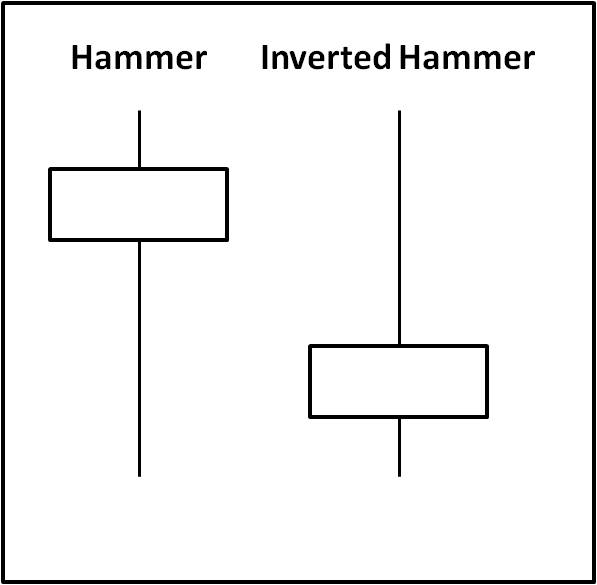
\includegraphics[width=5cm]{chp5e_candle_hammer}
\caption[Shooting Star.]{Hammer and Inverted Hammer.}
\label{fig:chp5e:hammer}
\end{figure}

Figure \ref{fig:chp5e:hammer} is a diagram of a Hammer and Inverted Hammer patterns. Both patterns have a small \textquotedblleft body" (the distance between the open and close prices) and a long \textquotedblleft shadow" (the distance between the high and low prices). In the diagrams presented here a white candlestick means the market price increased over the course of the day while a black one means the market fell. The body of the candlestick is white in this case, indicating that the market moved up (the closing price was above the opening price), although by only a small amount. Hammer and Inverted Hammer differ in that the long shadow in hammer is generated from a low price whereas the shadow of Inverted Hammer goes upwards as it is indicative of the period's high price.

\begin{figure}[tbph]
\centering
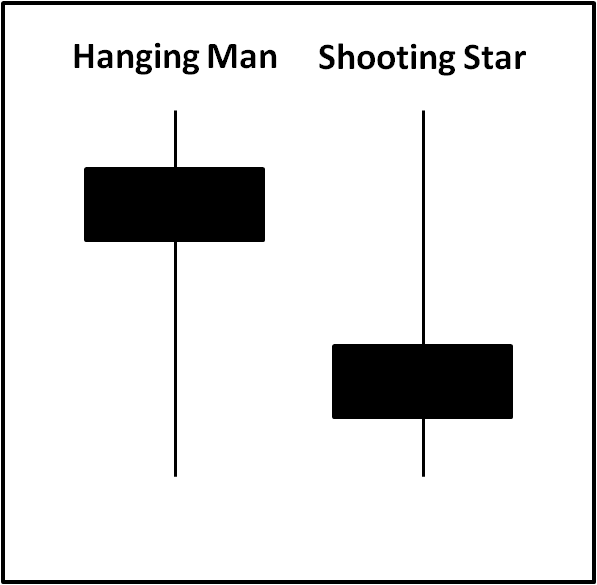
\includegraphics[width=5cm]{chp5e_candle_shoot_star}
\caption[Shooting Star.]{Shooting Star and Hanging Man.}
\label{fig:chp5e:shoot_star}
\end{figure}

Figure \ref{fig:chp5e:shoot_star} is a diagram of Hanging Man and Shooting Star, these being the opposite to Hammer and Inverted Hammer. In this case the market direction is down, albeit only by a small amount, and thus the body of the candlestick is a different colour, in this case black. Again both patterns have long shadows, the direction of which determines if the pattern is Hanging Man or Shooting Star.

\begin{figure}[tbph]
\centering
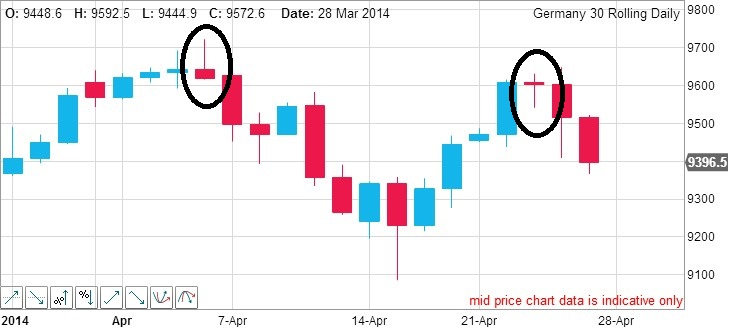
\includegraphics[width=12cm]{chp5e_candle_shoot_star_apr_dax_jp}
\caption [Dax Candlestick Patterns April 2014.]{Daily candlestick patterns from the German Dax over 22 days in April 2014 with Shooting Star and Hanging Man circled.}
\label{fig:chp5e:shoot_star_dax}
\end{figure}

Both sets of patterns Hammer/Inverted Hammer and Hanging Man/Shooting Star are considered to indicate that a trend is coming to a close and a reversal could be looming. In the case of Hammer/Inverted Hammer if they are encountered during a down trend they could indicate that the selling pressure is easing and a market move to the upside could happen soon. The opposite is true for Hanging Man/Shooting Star. When these are encountered in an up trend they often indicate that the trend is ending and a reversal may occur. Figure \ref{fig:chp5e:shoot_star_dax} shows daily candlestick patterns for the German Dax over 22 days in April 2014. A Shooting Star is circled on the 6th April and a Hanging Man on the 23rd April. In each case they occur while the market is rising and in each case it reverses immediately afterwards.

In order to have a system based on candlestick patterns, the pattern itself must be identified in code. A Hammer and Hanging Man are essentially the same pattern except Hammer has a close higher than the open whereas Hanging Man represents a decline in the price. For these patterns three components are defined, the length of the upper shadow (short), the size of the body (short) and the length of the lower shadow. In the trading system that follows these were defined as:

\begin{enumerate}
\item Upper Shadow - the value of the day's high minus the high of the body is less than 10\% the total High-Low range.
\item Body - is larger than 10\% the total High-Low range.
\item Lower Shadow - the value of the day's low minus the low of the body is greater than 66\% of the High-Low range.
\end{enumerate}

Analysing the Dax data set running from 2000 to 2013 with 3570 observations, and using the criteria described above 35 Hammer and 48 Hanging Man patterns can be detected. 

Inverted Hammer and Shooting Star are again the same pattern except in Inverted Hammer the price rose. In the later system these are defined as:

\begin{enumerate}
\item Upper Shadow - the value of the day's high minus the high of the body is at least 66\% the total High-Low range.
\item Body - is larger than 10\% the total High-Low range.
\item Lower Shadow - the value of the day's low minus the low of the body is less than 10\% of the High-Low range.
\end{enumerate}

Considering the Dax data set again, occurrences of these patterns are quite rare with 30 Inverted Hammers and 17 Shooting Stars in 3570 observations.

Results from a trading system based on the Hammer / Inverted Hammer can be seen in Table \ref{tab:hammer_results} and the R code in Appendix \ref{AppendixA} section \ref{appA:Hammer}. The algorithm simply places a buy the day after a Hammer or Inverted Hammer occur, the assumption being that these patterns indicate that the market is about to rise.


% latex table generated in R 3.1.0 by xtable 1.7-3 package
% Sat Jun 07 07:56:31 2014
\begin{table}[ht]
\centering
\caption[Hammer System]{Results from Hammer / Inverted Hammer.} 
\label{tab:hammer_results}
\begin{tabular}{lcccc}
  \toprule Mkt & LongPL & L Win \% & L Trades & Av L PL \\ 
  \midrule Dax & 594 & 53 & 126 & 5 \\ 
  CAC & -793 & 44 & 149 & -5 \\ 
  FTSE & 834 & 58 & 188 & 4 \\ 
  Dow & 2097 & 59 & 88 & 24 \\ 
  Nikkei & -2202 & 48 & 147 & -15 \\ 
  AORD & -809 & 46 & 236 & -3 \\ 
   \bottomrule \end{tabular}
\end{table}


An alternative approach is to look for Hammer and Inverted Hammer patterns occurring in a down trend, in which case it could signal the end of the down trend and the start of a reversal. Table \ref{tab:hammer_aroon_results} shows the results of using the Hammer and Inverted Hammer to predict a price rise during a down trend. An aroon down value of greater than 65 (with a 20 day look back period) is used to define the down trend. The algorithm can be seen in Appendix \ref{AppendixA} section \ref{appA:Hammer_aroon}.  


% latex table generated in R 3.1.0 by xtable 1.7-3 package
% Mon Jun 23 18:28:43 2014
\begin{table}[ht]
\centering
\caption[Results from a system based on the Hammer and Inverted Hammer candlestick patterns occurring in a downtrend]{Results from a system based on the Hammer and Inverted Hammer candlestick patterns occurring in a downtrend as defined by the aroon value.} 
\label{tab:hammer_aroon_results}
\begin{tabular}{lcccc}
  \toprule Mkt & LongPL & L Win \% & L Trades & Av L PL \\ 
  \midrule Dax & -187 & 42 & 36 & -5 \\ 
  CAC & -515 & 44 & 55 & -9 \\ 
  FTSE & 281 & 55 & 65 & 4 \\ 
  Dow & 730 & 55 & 22 & 33 \\ 
  Nikkei & -934 & 48 & 58 & -16 \\ 
  AORD & -614 & 41 & 77 & -8 \\ 
   \bottomrule \end{tabular}
\end{table}


%-------------------------------------------------------------
% -----------------  Engulfing Candlestick -------------------
\subsection{Engulfing Candlestick}
\label{sec:eng_cand}
The \textquotedblleft Engulfing" pattern, either Bull or Bear is another widely considered candlestick pattern and is depicted in Figure \ref{fig:chp5e:engulf}. This pattern has a lower low and a higher high than the preceding candlestick and is usually interpreted as indicating a change in direction of the trend. Engulfing candlesticks can be either bullish, where the closing price is above the opening price or bearish when the market moves down.

\begin{figure}[tbph]
\centering
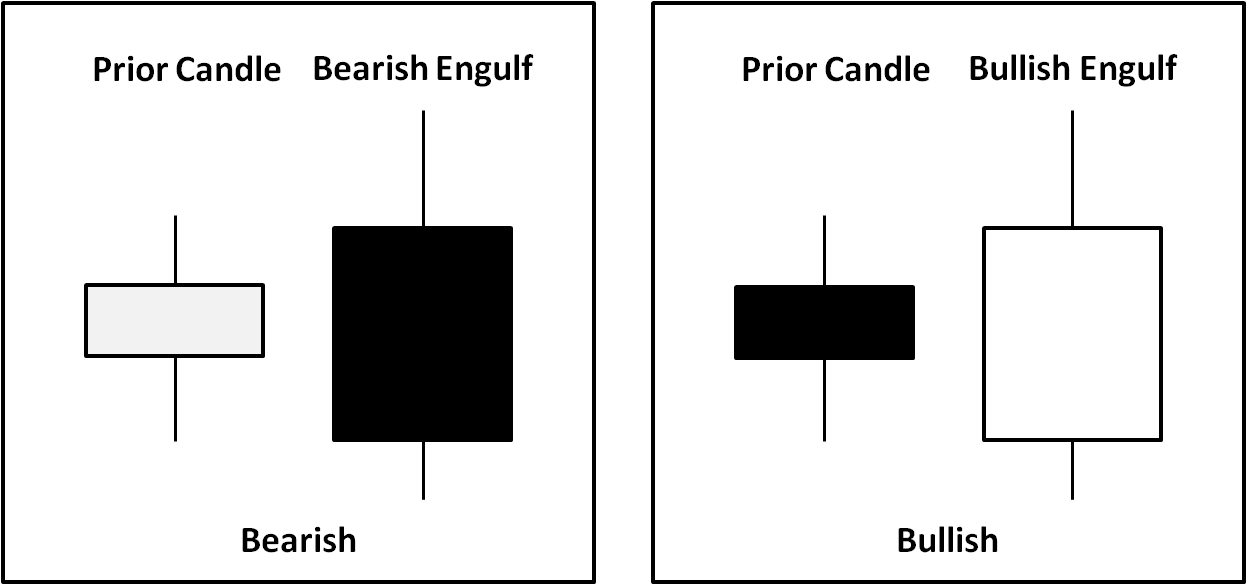
\includegraphics[width=10cm]{chp5e_candle_engulf}
\caption[ Engulfing Pattern.]{Engulfing Pattern.}
\label{fig:chp5e:engulf}
\end{figure}

Table \ref{tab:engulf_results} lists the results from passing a variety of national index data sets (see Appendix \ref{AppendixA} section \ref{appA:Engulf} for details) to an algorithm that buys or sells the market depending on the presence of an Engulfing pattern.


% latex table generated in R 3.1.0 by xtable 1.7-3 package
% Sun Aug 31 09:29:32 2014
\begin{table}[ht]
\centering
\caption[Results from a system based on the Engulfing candlestick pattern]{Results from a system based on the Engulfing candlestick pattern.} 
\label{tab:engulf_results}
\begin{tabular}{lcccccc}
  \toprule Mkt & LongPL & ShortPL & L Win \% & Av L PL & S Win \% & Av S PL \\ 
  \midrule DAX & -920 & -258 & 44 & -7 & 46 & -2 \\ 
  CAC & -319 & 228 & 45 & -2 & 50 & 1 \\ 
  FTSE & -1721 & 1185 & 51 & -4 & 50 & 3 \\ 
  Dow & -770 & -3662 & 48 & -4 & 35 & -28 \\ 
  Nikkei & -3823 & -1166 & 37 & -39 & 44 & -11 \\ 
  AORD & -6 & -600 & 53 & 0 & 46 & -3 \\ 
   \bottomrule \end{tabular}
\end{table}


Table \ref{tab:engulf_aroon_results} lists the results from extending the algorithm such that trades are only taken in either up or down trends, as defined by the aroon indicator. The R code for the amended algorithm can be see Appendix \ref{AppendixA} section \ref{appA:Engulf_aroon}.

% latex table generated in R 3.1.0 by xtable 1.7-3 package
% Sun Aug 31 09:29:33 2014
\begin{table}[ht]
\centering
\caption[Results from a system based on the Engulfing candlestick pattern in a trending market]{Results from a system based on the Engulfing candlestick pattern in a trending market.} 
\label{tab:engulf_aroon_results}
\begin{tabular}{lcccccc}
  \toprule Mkt & LongPL & ShortPL & L Win \% & Av L PL & S Win \% & Av S PL \\ 
  \midrule DAX & -874 & -513 & 38 & -20 & 43 & -7 \\ 
  CAC & -118 & -666 & 49 & -3 & 30 & -11 \\ 
  FTSE & -1217 & -782 & 47 & -8 & 48 & -3 \\ 
  Dow & 202 & -1154 & 45 & 4 & 44 & -11 \\ 
  Nikkei & -1522 & -1733 & 38 & -59 & 37 & -32 \\ 
  AORD & -49 & -27 & 53 & -1 & 50 & 0 \\ 
   \bottomrule \end{tabular}
\end{table}


%----------------------------------------------------------
% ---------------------------  Doji ------------------------
\subsection{Doji}
Doji is a well-known candlestick pattern that can appear on its own or as a component of a pattern. A Doji forms when the open and close price are similar and there is an upper and lower shadow, thus they often resemble a cross. Variations within Doji include the Dragonfly and Gravestone Doji, see Figure \ref{fig:chp5e:doji}. In an up trend Doji (especially Gravestone) can indicate a reversal could occur and likewise in a down trend a Dragonfly could suggest an upward move is about to start.

\begin{figure}[tbph]
\centering
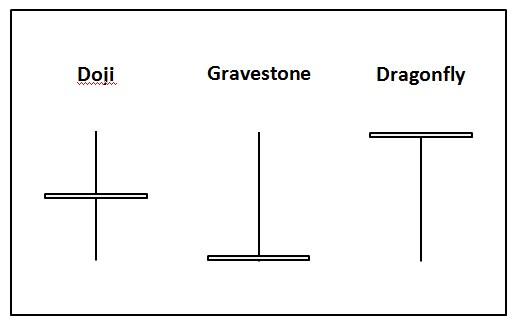
\includegraphics[width=10cm]{chp5e_candle_doji}
\caption[ Doji Star.]{Doji Pattern.}
\label{fig:chp5e:doji}
\end{figure}

Table \ref{tab:doji_aroon_results} lists the results from passing a variety of national index data sets (see Appendix \ref{AppendixA} section \ref{appA:Doji_aroon} for details) to an algorithm that buys or sells the market depending on the presence of a Doji. In an up trend, as identified by the aroon indicator, a Doji or Gravestone is used to initiate a sell and conversely in down trend a Doji or Dragonfly is used as a signal to buy.

% latex table generated in R 3.1.0 by xtable 1.7-3 package
% Thu Jul 10 21:16:47 2014
\begin{table}[ht]
\centering
\caption[Results from a system based on the Doji candlestick pattern in a trending market]{Results from a system based on the Doji candlestick pattern in a trending market.} 
\label{tab:doji_aroon_results}
\begin{tabular}{lcccccc}
  \toprule Mkt & LongPL & ShortPL & L Win \% & Av L PL & S Win \% & Av S PL \\ 
  \midrule Dax & -826 & -1132 & 53 & -8 & 52 & -6 \\ 
  CAC & -747 & -326 & 46 & -6 & 49 & -2 \\ 
  FTSE & -697 & 418 & 53 & -8 & 52 & 3 \\ 
  Dow & -763 & -2869 & 51 & -5 & 50 & -10 \\ 
  Nikkei & 1296 & -2944 & 55 & 12 & 45 & -22 \\ 
  AORD & -115 & 195 & 54 & -1 & 54 & 2 \\ 
   \bottomrule \end{tabular}
\end{table}

 

% Chapter 5

\chapter{Time Series} % Main chapter title

\label{Chapter5} % For referencing the chapter elsewhere, use \ref{Chapter5} 

\lhead{Chapter 5. \emph{Time Series}} % This is for the header on each page - perhaps a shortened title

%----------------------------------------------------------------------------------------

This chapter will explore the use of time series analysis techniques to generate models for forecasting prices in various national stock market indices. Usually, in trying to predict the future behaviour of financial markets the direction they will move, either up or down, is of more interest than the actual value itself. Thus, in this chapter predictions of the future direction as well as the actual value itself are attempted.  A variety of time series models are developed using exponential smoothing, ARIMA and hybrid ARIMA methods.

\section{Exponential Smoothing}

Exponential smoothing was applied to the stock market indice data sets in order to generate predictions for the following day's closing price, so-called one-step ahead forecasts. Two basic approaches and an exponential smoothing methodology were examined. The two basic methods provide a useful baseline against which to compare later models, and are the mean and drift methodologies. The mean is simply the average of the data points in the sample while the drift is equivalent to drawing a straight line between the first and last point of the sample and then extrapolating this line forward the desired number of observations.

\subsection{Time Series Base Models}
Figure \ref{fig:chp5_ts_dax} shows the two base methods, mean and drift, being applied to a data set derived from the German DAX. The models were trained on the first 3000 observations of the DAX data set and tested on the remaining ones. The actual data points being predicted in Figure \ref{fig:chp5_ts_dax} are added to the plot in Figure \ref{fig:chp_ts_dax_act}. Five error measures, root mean square error (RMSE), mean absolute error (MAE), mean percentage error (MPE), mean absolute percentage error (MAPE) and mean absolute scaled error (MASE) for the two methods are listed in Table \ref{tab:chp_ts:sma}. From these error measures we can see that the drift model fits the training data the best, having the smallest error values across all the measures, but that the mean model actually performs the best on the test data.

%label - tab:chp_ts:sma
% latex table generated in R 3.1.0 by xtable 1.7-3 package
% Tue May 27 13:22:33 2014
\begin{table}[ht]
\centering
\caption[Simple forecasting methods.]{Mean, Naive and Drift methods applied to 
         to the Dax.} 
\label{tab:chp_ts:sma}
\begin{tabular}{llcccc}
  \toprule  & RMSE & MAE & MPE & MAPE & MASE \\ 
  \midrule Mean Training Set & 1394 & 1183 & -8 & 25 & 1 \\ 
  Mean Test Set & 208 & 163 & 2 & 3 & 3 \\ 
  Naive Training Set & 84 & 61 & -0 & 1 & 0 \\ 
  Naive Test Set & 303 & 263 & -5 & 5 & 4 \\ 
  Drift Training Set & 84 & 61 & -0 & 1 & 0 \\ 
  Drift Test Set & 302 & 262 & -5 & 5 & 4 \\ 
   \bottomrule \end{tabular}
\end{table}


\begin{figure}[tbh]
\centering
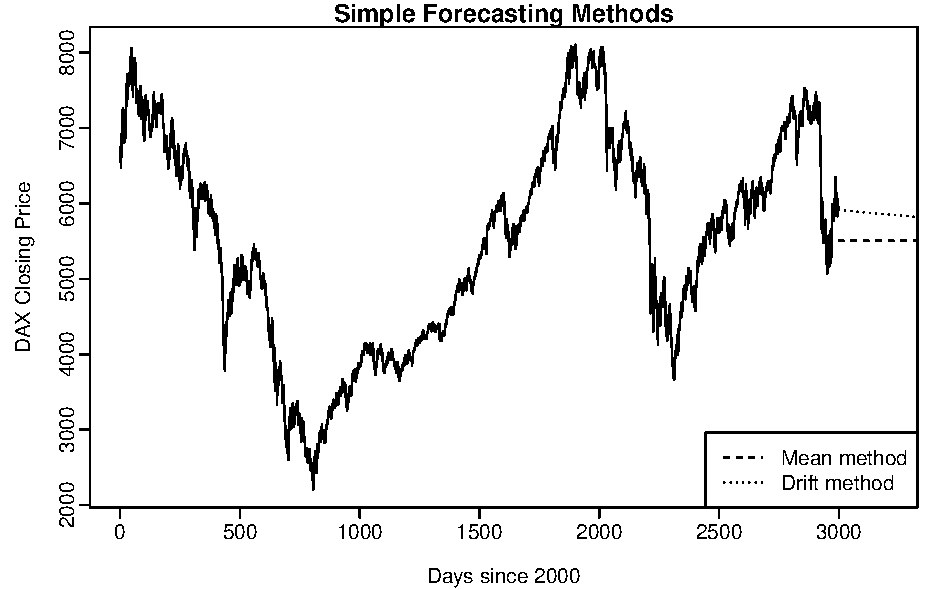
\includegraphics{Figures/chp_ts_dax1}
\caption[Forecasts generated by mean and drift methods]{Forecasts generated by mean and drift methods.}
\label{fig:chp5_ts_dax}
\end{figure}

\begin{figure}[tbh]
\centering
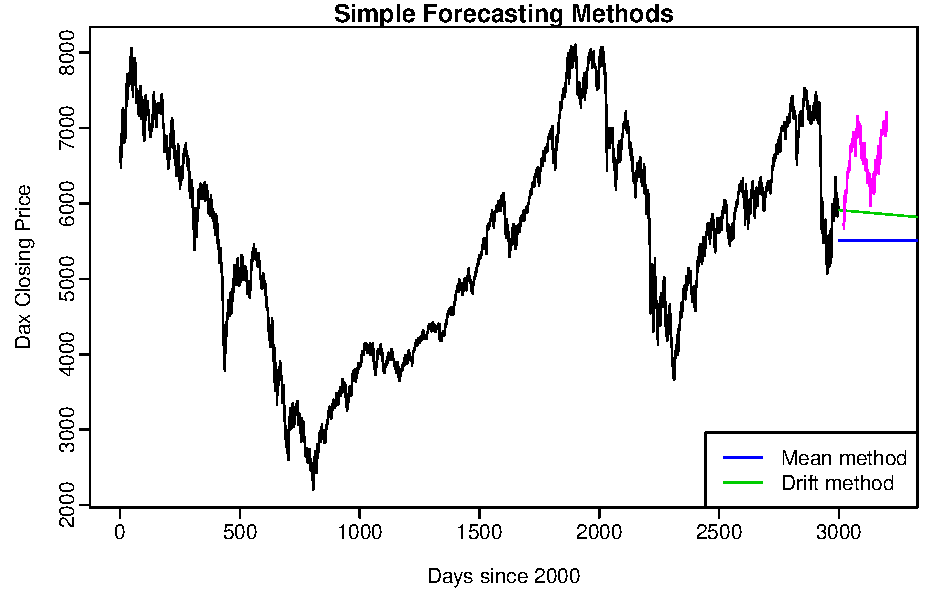
\includegraphics{Figures/chp_ts_dax1_plus_act_data}
\caption[Forecasts generated by mean and drift methods and actual data]{Forecasts generated by mean and drift methods with actual data in forecast period added.}
\label{fig:chp_ts_dax_act}
\end{figure}

Looking at Figure \ref{fig:chp_ts_dax_act} it can be seen that neither the mean or the drift does a good job with the predictions for the DAX. The forecasts were based on the entire data set, treating it as a homogeneous whole. However, financial time series typically show a variety of behaviour at different periods. On occasions it is stationary and at other times trending. Thus, in the following sections, in order to generate forecasts a sliding window approach was adopted. A window of data (the last 30 observations) was used to generate a model and the one-step ahead forecast, before the window was advanced one observation to the next period. In this way the model is constantly adapting and changing. Using this approach forecasts and models for use in a trading system from a mean, drift and exponential smoothing methodology were developed.

\subsection{Trading System Based on Mean Model}
\label{sec:es:mean}
Results from a trading system using the one-step ahead forecasts generated by the mean model using a moving window are listed in Table \ref{tab:es_mean_sys}. A trading algorithm, which can be seen in Appendix \ref{AppendixA} section \ref{appA:es_1}, used these forecasts to decide in which direction to trade. If the forecast was higher than the closing price a long trade was entered the following day and likewise if it was below the close a short trade was entered.


%label - tab:es_mean_sys
% latex table generated in R 3.1.0 by xtable 1.7-3 package
% Mon Jul 07 20:34:26 2014
\begin{table}[ht]
\centering
\caption[Results from the mean base ES System]{Results from the mean base ES System.} 
\label{tab:es_mean_sys}
\begin{tabular}{lcccccc}
  \toprule Mkt & LongPL & ShortPL & L Win \% & Av L PL & S Win \% & Av S PL \\ 
  \midrule Dax & -1640 & -1505 & 50 & -1 & 45 & -1 \\ 
  CAC & -1086 & 3553 & 52 & -1 & 51 & 2 \\ 
  FTSE & 1680 & 345 & 53 & 1 & 49 & 0 \\ 
  Dow & 8356 & -2126 & 54 & 7 & 46 & -1 \\ 
  Nikkei & -32 & 10646 & 51 & 0 & 53 & 6 \\ 
  AORD & -1333 & -2149 & 50 & -1 & 46 & -1 \\ 
   \bottomrule \end{tabular}
\end{table}


\subsection{Trading System Based on Drift Model}
In a similar way to the mean model of section \ref{sec:es:mean} the predictions generated by the drift model were passed to the trading algorithm and the results can be seen in Table \ref{tab:es_drift_sys}. 

%label - tab:es_drift_sys
% latex table generated in R 3.1.0 by xtable 1.7-3 package
% Thu Jul 10 20:50:38 2014
\begin{table}[ht]
\centering
\caption[Results from the drift base ES System]{Results from the drift base ES System.} 
\label{tab:es_drift_sys}
\begin{tabular}{lcccccc}
  \toprule Mkt & LongPL & ShortPL & L Win \% & Av L PL & S Win \% & Av S PL \\ 
  \midrule Dax & 2310 & 2445 & 54 & 1 & 50 & 2 \\ 
  CAC & -2422 & 2217 & 49 & -1 & 48 & 2 \\ 
  FTSE & -518 & -1853 & 51 & 0 & 47 & -1 \\ 
  Dow & 5416 & -5066 & 54 & 3 & 46 & -4 \\ 
  Nikkei & -6939 & 3739 & 48 & -4 & 50 & 3 \\ 
  AORD & 1476 & 660 & 53 & 1 & 49 & 1 \\ 
   \bottomrule \end{tabular}
\end{table}


\subsection{Trading System Based on Exponential Smoothing Model}

Using Rob J Hyndman's forecast package and the ets function, a variety of exponential smoothing methods can be applied to sample data \citep{Hyndman08automatictime}. Table \ref{tab:tax_em} lists fifteen possibilities when one combines trend and seasonality, both additive and multiplicative. In fact Hyndman extends this further by allowing the error term to be either added or multiplied against the results. 

\begin{table}[ht]
\centering
\caption[Taxonomy of exponential smoothing methods]{Taxonomy of exponential smoothing methods.} 
\label{tab:tax_em}
\begin{tabular}{lccc}
  \toprule 
            & \multicolumn{3}{c}{Seasonal Component} \\
  \cmidrule(r){2-4}
  Trend     & N      & A          & M       \\ 
  Component &(None)  &(Additive)  & (Multiplicative)  \\
  \midrule 
  N (None) & (N,N)&(N,A)&(N,M)  \\ 
  A (Additive) & (A,N)&	(A,A)&(A,M)  \\ 
  Ad (Additive damped) &(Ad,N)&(Ad,A)&(Ad,M) \\ 
  M (Multiplicative) &(M,N)&(M,A)&(M,M)  \\ 
  Md (Multiplicative damped) &(Md,N)&(Md,A)&(Md,M) \\ 
   \bottomrule \end{tabular}
\end{table}

%Note - Hymndman: hard to beat the ets model, 37 mins.

Using a sliding window approach, one-step ahead forecasts were generated using the ets function. Because a different sample of data was contained in each window, the exponential smoothing function selects the best model for each window of data independently of the data set as a whole. Thus the ets function applies a variety of models to the windows of data including:

\begin{itemize}
\item ETS(A,N,N)
\item ETS(M,N,N)
\item ETS(M,A,N)
\item ETS(A,A,N)
\item ETS(A,Ad,N)
\item ETS(M,Md,N)
\item ETS(M,Ad,N)
\item ETS(M,M,N)
\end{itemize}


The one-step ahead forecasts generated from these models were once again passed to the same trading algorithm listed in Appendix \ref{AppendixA} section \ref{appA:es_1} and the results can be seen in Table \ref{tab:es_sys}.

%label - tab:es_sys
% latex table generated in R 3.1.0 by xtable 1.7-3 package
% Sat Aug 23 08:35:08 2014
\begin{table}[ht]
\centering
\caption[Results from trading the predictions generated by a moving window exponential smoothing system]{Results from trading the predictions generated by a moving window exponential smoothing system.} 
\label{tab:es_sys}
\begin{tabular}{lcccccc}
  \toprule Mkt & LongPL & ShortPL & L Win \% & Av L PL & S Win \% & Av S PL \\ 
  \midrule DAX & -2029 & -1894 & 53 & -1 & 47 & -1 \\ 
  CAC & -266 & 4048 & 52 & 0 & 51 & 2 \\ 
  FTSE & 3866 & 2531 & 53 & 3 & 50 & 2 \\ 
  Dow & 12901 & 2419 & 57 & 8 & 50 & 2 \\ 
  Nikkei & -2741 & 7937 & 49 & -2 & 51 & 5 \\ 
  AORD & 645 & -171 & 52 & 0 & 48 & 0 \\ 
   \bottomrule \end{tabular}
\end{table}


% ------ NEW PAGE --------------------------
%\newpage
\section{ARIMA Models}
\label{arima_models}
The use of Auto-Regressive Integrated Moving Average (ARIMA) models, see section \ref{sec:arima} for details, was explored in order to forecast future prices for financial markets. 
The process of fitting an ARIMA model to a time series is quite challenging and involves the following general steps:

\begin{enumerate}
\item Plot the data to get a general feel for the time series and to establish if it is stationary.
\item Stabilize any variance in the data with a transformation process such as the Box-Cox method.
\item ARIMA models work with stationary data, so if necessary, take differences of the data until it is stationary.
\item Examine the auto-correlation and partial auto-correlation (ACF/PACF) plots in order to determine if an AR(p) or MA(q) model is appropriate.
\item Test the chosen model(s), using the AICc to determine if a better model is available.
\item Check the residuals from the best model by plotting the ACF, and doing a portmanteau test on them. If the results from these tests do not look like white noise, a modified model may be required.
\item Finally, once the residuals have a similar pattern to white noise, the model can be used to generate forecasts.
\end{enumerate}


In recent years automatic forecasting algorithms have become available and are widely used \citep{Hyndman08automatictime}. These are necessary in a variety of circumstances, especially when organisations are faced with the need to repeatedly carry out a large number of forecasts and the human effort required renders manual means impractical. The auto.arima function found in R's \textquotedblleft forecast" package is an example of an automatic algorithm for ARIMA models. This function automates steps 3, 4, and 5 of those outlined previously, in the general steps required for ARIMA modelling. In the following sections, the general steps are used to generate an ARIMA model manually, and then the automatic algorithm is utilised to build one.

\section{Manual Generation of ARIMA Models}
\label{sec:man_arima}
\subsection{Data Exploration}

The first step, as always is to explore the data. Figure \ref{fig:chp_ts_ftse_2000_13} shows the UK's FTSE 100 index between the years 2000 to 2013. Over this time period the series has shown strong trends to move up and down and a uniform variance. Because the time series is non-stationary it will need to be transformed into a stationary series before ARIMA modelling can be undertaken.

\begin{figure}[tbh]
\centering
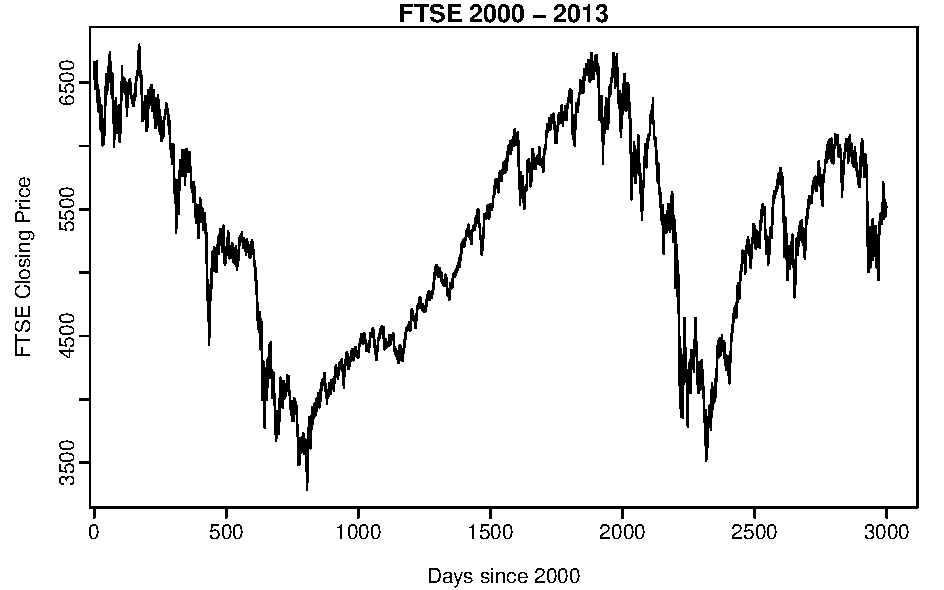
\includegraphics{Figures/chp_ts_ftse_2000-13}
\caption[FTSE 100 index between the years 2000 to 2013]{UK's FTSE 100 index between the years 2000 to 2013.}
\label{fig:chp_ts_ftse_2000_13}
\end{figure}

\subsection{Adjusting for non-uniform variance and non-stationariness}
The variance within the FTSE time series is relatively uniform and thus this data set doesn't need stabilizing with regard to this. If it did, a Box-Cox transformation could be used. However, over this time period the FTSE 100 exhibits marked non-stationariness and requires adjusting accordingly. One such technique to make a data set stationary is differencing. Instead of using the actual observations the differences between two adjacent points are used and this is known as the first difference. If the data set still isn't stationary the difference between consecutive points in the differenced data set can used, this is the difference of the differences and is known as the second difference. Figure \ref{fig:chp_ts_ftse_2000_13_diff} shows the FTSE data set after the first differences have been taken.  The resulting data set is now stationary.

\begin{figure}[tbh]
\centering
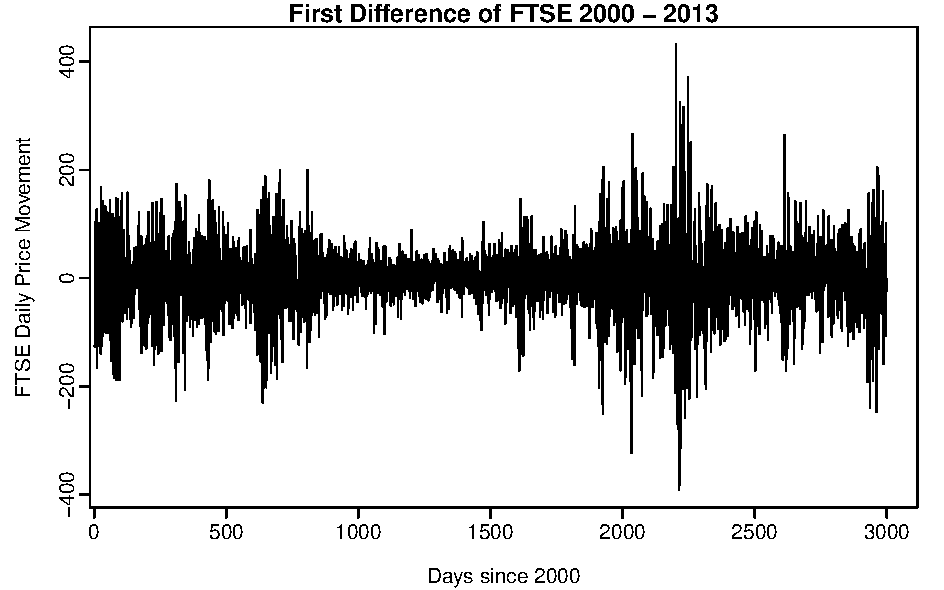
\includegraphics{Figures/chp_ts_ftse_2000-13_diff}
\caption[First difference of FTSE 100 between the years 2000 to 2013]{First difference of FTSE 100 between the years 2000 to 2013.}
\label{fig:chp_ts_ftse_2000_13_diff}
\end{figure}

\subsection{Examine ACF/PACF}
With a stationary data set, the next stage is to investigate the auto-correlation and partial auto-correlation (ACF/PACF) plots in order to help in the model selection process (see section \ref{sec:acf} for details of ACF and PACF). The ACF and PACF for the FTSE data set can be seen in Figures \ref{fig:chp_ts_ftse_2000-13_diff_acf} and \ref{fig:chp_ts_ftse_2000-13_diff_pacf}. 

If ultimately the ARIMA model is of the form ARIMA(p,d,0) or ARIMA(0,d,q) then the ACF and PACF plots are useful in helping to define values for p or q. In the event that both p and q are positive, the ACF and PACF are not helpful in deducing the values for p and q. An ARIMA(p,d,0) model may be appropriate if the ACF and PACF plots of the stationary data exhibit an exponentially decaying pattern in the ACF and a large spike at lag p in PACF plot. Conversely an ARIMA(0,d,q) model may be appropriate if the PACF is decaying exponentially and there is there is a significant spike in the ACF plot at lag q. Considering the ACF and PACF plots in Figures \ref{fig:chp_ts_ftse_2000-13_diff_acf} and \ref{fig:chp_ts_ftse_2000-13_diff_pacf}, neither of the two patterns are observed and thus an ARIMA model where both p and q are positive is likely.

\begin{figure}[tbh]
\centering
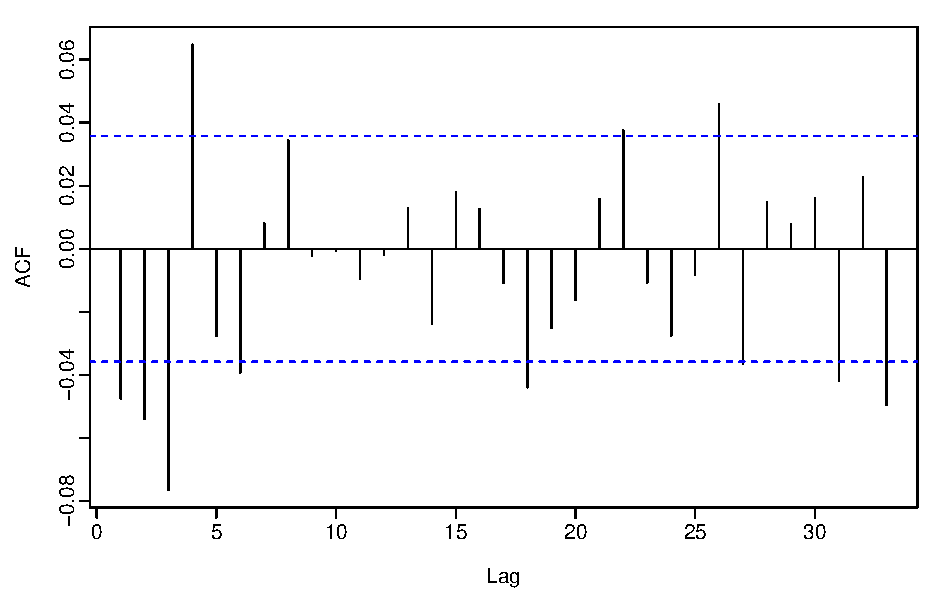
\includegraphics{Figures/chp_ts_ftse_2000-13_diff_acf}
\caption[ACF of FTSE 100 between the years 2000 to 2013]{Auto-correlation plot of differenced data from FTSE 100 between the years 2000 to 2013.}
\label{fig:chp_ts_ftse_2000-13_diff_acf}
\end{figure}

\begin{figure}[tbh]
\centering
\includegraphics{Figures/chp_ts_ftse_2000-13_diff_pacf}
\caption[PACF of FTSE 100 between the years 2000 to 2013]{Partial auto-correlation plot of differenced data from FTSE 100 between the years 2000 to 2013.}
\label{fig:chp_ts_ftse_2000-13_diff_pacf}
\end{figure}

%\begin{figure}[tbh]
%\centering
%%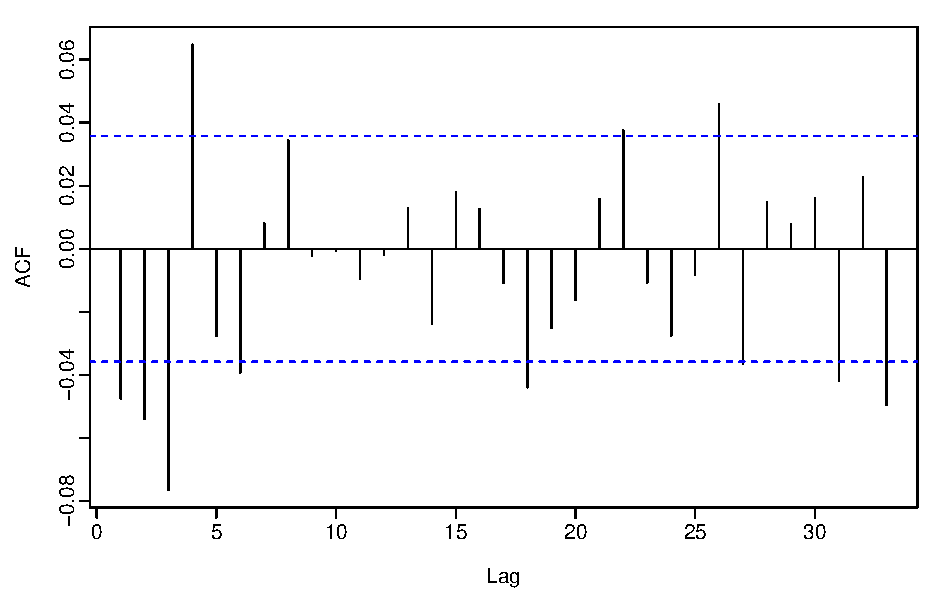
\includegraphics[width=15cm]{Figures/chp_ts_ftse_2000-13_diff_acf}
%\includegraphics[width=14cm, height=12cm]{Figures/chp_ts_ftse_2000-13_diff_acf_tsd}
%\caption[FTSE 2000-13 ACF / PACF.]{Difference, ACF and PACF plots for the FTSE 2000-13.}
%\label{fig:chp_ts_ftse_2000_13_diff_acf_tsd}
%\end{figure}
\textquotesingle\newpage
\subsection{Try the chosen model(s)}
The next step is to try the chosen model along with a few viable alternatives. Akaike’s Information Criterion (AIC) and Bayesian Information Criterion (BIC) are useful for determining the optimum order of an ARIMA model, and are typically used as a measure of how well the model fits the data. AIC can be given by:

\[ AIC = -2 log (L) + 2 (p+q+k+1) \]
where:\\
$ L $ is the likelihood of the data and $ k = 1$ if $c\neq0$ and $ k=0$ if $c \neq 0$, the last term in parentheses is the number of parameters in the model.

For ARIMA models, the corrected AIC can be written as:
\[ AIC_{c} = AIC + \dfrac{2 (p+q+k+1)(p+q+k+2)}{T-p-q-k-2} \]

The Bayesian Information Criterion can be expressed as:
\[ BIC = AIC + log(T)(p+q+k+1) \]

Table \ref{tab:chp_ts:arima_res_r} shows the AIC, AICc and BIC accuracy measures for a selection of ARIMA models applied to the FTSE data set. On all three measures the ARIMA(2,1,3) model has the lowest value.

%label - tab:chp_ts:arima_res_r
% latex table generated in R 3.1.0 by xtable 1.7-3 package
% Thu Aug 21 07:23:05 2014
\begin{table}[ht]
\centering
\caption[AIC, AICc and BIC results from alternative ARIMA models]{AIC, AICc and BIC results from alternative ARIMA models.} 
\label{tab:chp_ts:arima_res_r}
\begin{tabular}{lccc}
  \toprule Model & AIC & AICc & BIC \\ 
  \midrule ARIMA(3,1,1) & 33598.5 & 33598.5 & 33628.5 \\ 
  ARIMA(3,1,2) & 33594.6 & 33594.6 & 33630.6 \\ 
  ARIMA(3,1,3) & 33596.1 & 33596.1 & 33638.1 \\ 
  ARIMA(2,1,1) & 33616.4 & 33616.4 & 33640.4 \\ 
  ARIMA(2,1,2) & 33618.1 & 33618.1 & 33648.1 \\ 
  ARIMA(2,1,3) & 33594.1 & 33594.1 & 33630.1 \\ 
   \bottomrule \end{tabular}
\end{table}


\subsection{Model Residuals}
A so-called residual is the difference between an observation and its forecast. In forecasting a time series, residuals are calculated from a one-step forecast.  A one-step forecast is based on all observations from the start of the series until the previous observation to which the forecast applies to. Thus the number of data points used to calculate the one-step forecast increases as the forecast proceeds through the time series.  An alternative is cross-sectional forecasting which uses all the points in the data set except the observation being predicted.

Knowledge of the residuals from the application of a model is important in establishing the validity of the model. There are two essential and two valuable properties that can be established by inspecting the model residuals. A good method of forecasting will produce a model in which the residuals are uncorrelated and have a zero mean. If a forecasting method doesn't comply with these two properties it can be improved upon. Correlation in residuals means that information is present in them that the model has missed and a non-zero mean is evidence of bias in the forecast. Adjusting for bias is straight forward, the mean value observed in the residuals can simply be added to all forecasts. Looking at Figure \ref{fig:chp_ts_ftse_2000_13_mean_residuals} it can be seen that the mean of the residuals is close to zero and this model doesn't have any bias. Figure \ref{fig:chp_ts_ftse_2000_13_acf_residuals} is the plot of the residuals of the ARIMA model applied to the FTSE data set. The lower order lags are all within the confidence boundaries and is indicative of a good model.

\begin{figure}[!tbh]
\centering
\includegraphics{Figures/chp_ts_ftse_2000-13_mean_residuals}
\caption[FTSE 100 ARIMA model residuals.]{The residuals after applying the ARIMA(2,1,3) model to the FTSE data set.}
\label{fig:chp_ts_ftse_2000_13_mean_residuals}
\end{figure}

\begin{figure}[!tbh]
\centering
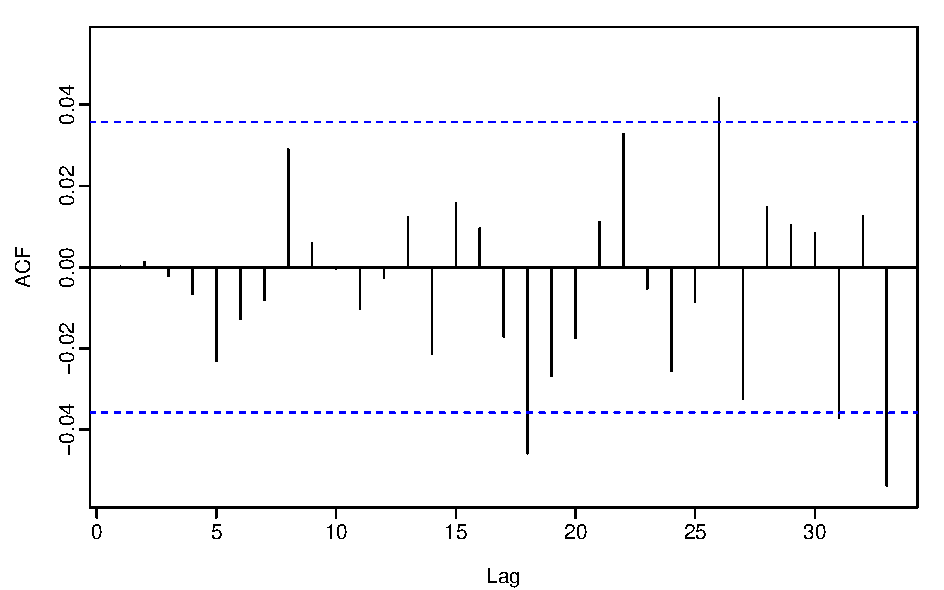
\includegraphics{Figures/chp_ts_ftse_2000-13_acf_residuals}
\caption[ACF plot of the FTSE 100 ARIMA model residuals]{ACF plot of the residuals after applying the ARIMA(2,1,3) model to the FTSE data set.}
\label{fig:chp_ts_ftse_2000_13_acf_residuals}
\end{figure}

Two additional properties of the residuals that are desirable, though not necessary, are constant variance and normal distribution. If these two conditions are met, the calculation of the prediction interval in the forecast step is easier. From Figure \ref{fig:chp_ts_ftse_2000_13_mean_residuals} it can be seen that the residuals have relatively constant variance and from Figure \ref{fig:chp_ts_ftse_2000_13_hist_residuals}, a histogram of the residuals, it can be seen that they are normally distributed.

\begin{figure}[!tbh]
\centering
\includegraphics{Figures/chp_ts_ftse_2000-13_hist_residuals}
\caption[Histogram of the FTSE 100 ARIMA model residuals]{Histogram of the residuals after applying the ARIMA(2,1,3) model to the FTSE data set.}
\label{fig:chp_ts_ftse_2000_13_hist_residuals}
\end{figure}

% Box Ljung test
Consideration of the ACF plots provides evidence for auto-correlation. However a more formal approach is to consider auto-correlation values together as a group as opposed to individually. The Box-Ljung portmanteau test is just one such approach and Table \ref{tab:chp_ts:arima_res_rbox_l} lists the results of the Box-Ljung portmanteau test being applied to the residuals of the ARIMA(2,1,3) model. A large p-value is indicative of white noise and is the desirable situation for a good ARIMA model. Taking all the evidence together the ARIMA(2,1,3) model appears a good option for the FTSE data set.

%label - tab:chp_ts:arima_res_rbox_l
% latex table generated in R 3.1.0 by xtable 1.7-3 package
% Mon Jul 07 19:17:49 2014
\begin{table}[ht]
\centering
\caption[Box Ljung test of FTSE 100 ARIMA model residuals]{Box Ljung test of FTSE 100 ARIMA model residuals.} 
\label{tab:chp_ts:arima_res_rbox_l}
\begin{tabular}{llcc}
  \toprule  & p-value & x-squared & df \\ 
  \midrule ARIMA(2,1,3)                    & 0.2328 & 20 & 24 \\ 
   \bottomrule \end{tabular}
\end{table}


\subsection{Calculate forecast}
Finally, after developing a model that meets the previous criteria a forecast can be generated. Table \ref{tab:chp_ts:ftse_100_fcast} shows the one-step forecast produced when the ARIMA(2,1,3) model developed in the previous section is applied to the FTSE data set.
 
%label - tab:chp_ts:ftse_100_fcast
% latex table generated in R 3.1.0 by xtable 1.7-3 package
% Tue Aug 26 19:01:45 2014
\begin{table}[ht]
\centering
\caption[Forecast for FTSE 100 generated from the ARIMA model]{One-step ahead forecast for FTSE 100 generated from ARIMA(2,1,3) model.} 
\label{tab:chp_ts:ftse_100_fcast}
\begin{tabular}{lccccc}
  \toprule Date & Open & High & Low & Close & Forecast \\ 
  \midrule 20/12/2013 & 6585 & 6617 & 6577 & 6607 & 6560 \\ 
  23/12/2013 & 6607 & 6679 & 6606 & 6679 & 6598 \\ 
  24/12/2013 & 6679 & 6712 & 6672 & 6694 & 6666 \\ 
  27/12/2013 & 6694 & 6754 & 6694 & 6751 & 6692 \\ 
  30/12/2013 & 6751 & 6768 & 6718 & 6731 & 6743 \\ 
  31/12/2013 & 6731 & 6757 & 6731 & 6749 & 6730 \\ 
   \bottomrule \end{tabular}
\end{table}


\section{Automatic Generation of ARIMA Models}
As explained previously the automatic ARIMA modelling algorithm in the R forecast package, auto.arima, automates steps 3 to 5 in the general steps used in the modelling process as outlined in section \ref{arima_models}. The function uses a variation of the Hyndman and Khandakar algorithm which obtains an ARIMA model by the minimisation of the AICc and combination with unit root tests. KPSS tests are used to establish the number of differences, d, required to get a stationary time series. The p and q values are then obtained by choosing the model that minimises the AICc for the differenced data. 

The results of passing the indice data sets to the auto.arima function can be seen in Table \ref{tab:chp_ts_arima_models}. For the FTSE data set the automatic procedure selects the ARIMA(2,1,3) as being the most appropriate, which matches the conclusion of the work from the manual model selection process described earlier in section \ref{sec:man_arima}.

%label - tab:chp_ts_arima_models
% latex table generated in R 3.1.0 by xtable 1.7-3 package
% Sat Aug 23 08:35:18 2014
\begin{table}[ht]
\centering
\caption[ARIMA models chosen for the indice data sets]{ARIMA models chosen to forecast future values in the national indice data sets.} 
\label{tab:chp_ts_arima_models}
\begin{tabular}{lc}
  \toprule Market & ARIMA Model \\ 
  \midrule DAX & ARIMA(3,1,3)                    \\ 
  CAC & ARIMA(2,1,3)                    \\ 
  FTSE & ARIMA(2,1,3)                    \\ 
  Dow & ARIMA(1,1,2)                    \\ 
  Nikkei & ARIMA(2,1,3)                    \\ 
  AORD & ARIMA(1,1,0)                    \\ 
   \bottomrule \end{tabular}
\end{table}


\section{Trading the ARIMA Models}
\label{sec:traing:arima:models}
Having developed forecasts based on ARIMA models these can be passed into a trading system. Two ideas are presented here, in the first the previous closing price is compared against the prediction and if it is lower than the forecast a long trade is entered. This first system will be referred to as System 1. In the second algorithm the current forecast is compared with the previous prediction. When the previous forecast value is lower than the current prediction the system trades long. This algorithm will be referred to as System 2.

The data sets containing fourteen years of indice data was divided into a training set, containing the first ten years of data, and a test set holding the remaining four years worth of data. Models were trained on the training sets before being applied to the unseen data in the test sets.

\subsection{System 1 - Close Price vs Forecast}
Using the ARIMA models listed in Table \ref{tab:chp_ts_arima_models} a series of amended data sets were generated by applying the models to the national indice data sets used throughout this study. The amended data sets contained the original Date, Open, High, Low and Close attributes plus a new one called Forecast, in a similar manner to the data seen in Table  \ref{tab:chp_ts:ftse_100_fcast}. Table \ref{tab:chp_ts:arima1} are results produced from passing the newly generated data sets to the algorithm listed in Appendix \ref{AppendixA} section \ref{appA:ts_1}. This system uses the relative position of the close price and the forecast to determine the direction of the trade. If the forecast is higher than the close a long trade is made the next day and when the prediction is lower than the close price a short trade is made.

%label - tab:chp_ts:arima1
% latex table generated in R 3.1.0 by xtable 1.7-3 package
% Sun Jun 29 08:18:19 2014
\begin{table}[ht]
\centering
\caption[Forecasts generated by the ARIMA models used in the System 1 algorithm]{Forecasts generated by the ARIMA models used in the System 1 algorithm.} 
\label{tab:chp_ts:arima1}
\begin{tabular}{lcccccc}
  \toprule Mkt & LongPL & ShortPL & L Win \% & Av L PL & S Win \% & Av S PL \\ 
  \midrule Dax & -644 & -1881 & 50 & -3 & 41 & -7 \\ 
  CAC & 1555 & 850 & 59 & 6 & 51 & 3 \\ 
  FTSE & 531 & -708 & 53 & 2 & 46 & -2 \\ 
  Dow & 3130 & -1766 & 58 & 14 & 48 & -6 \\ 
  Nikkei & 41 & -1157 & 48 & 0 & 45 & -5 \\ 
  AORD & 679 & -204 & 55 & 3 & 49 & -1 \\ 
   \bottomrule \end{tabular}
\end{table}


\subsection{System 2 - Forecast vs Previous Forecast}
Table \ref{tab:chp_ts:arima2} lists the results from passing the amended indice data sets with the forecasts generated from the auto.arima function, described in the previous section, to the System 2 algorithm. The R code of this system can be seen in  Appendix \ref{AppendixA} section \ref{appA:ts_2}. System 2 uses the relative values of the forecasts themselves to decide which direction to trade. If the prediction is higher than the previous day's prediction a long trade is initiated the following day and in the opposite circumstances when the previous forecast is higher than the current forecast a short trade is made.

%label - tab:chp_ts:arima2
% latex table generated in R 3.1.0 by xtable 1.7-3 package
% Tue Aug 19 13:19:29 2014
\begin{table}[ht]
\centering
\caption[Results from trading System 2 using the forecasts generated by the ARIMA models]{Results from trading System 2 using the forecasts generated by the ARIMA models.} 
\label{tab:chp_ts:arima2}
\begin{tabular}{lcccccc}
  \toprule Mkt & LongPL & ShortPL & L Win \% & Av L PL & S Win \% & Av S PL \\ 
  \midrule DAX & 733 & -505 & 55 & 3 & 46 & -2 \\ 
  CAC & 545 & -80 & 53 & 2 & 47 & 0 \\ 
  FTSE & 941 & -383 & 54 & 3 & 46 & -2 \\ 
  Dow & 2598 & -2221 & 55 & 9 & 46 & -10 \\ 
  Nikkei & 179 & -916 & 50 & 1 & 47 & -4 \\ 
  AORD & 811 & -117 & 53 & 3 & 46 & 0 \\ 
   \bottomrule \end{tabular}
\end{table}

% ---------------------------------------------------------------
\section{Hybrid ARIMA Models}
\label{sec:arima:chp5}
A hybrid ARIMA model is one in which the moving averages of a stationary data set (possibly a non-stationary data set that has been differenced) are combined with data mining learners other than regression. A variety of combinations were tried, with a combination of the three previous closing prices and differences and the four previous moving averages providing good results. Possible learners include k-Nearest Neighbour (k-NN) algorithms, Artificial Neural Networks (ANN) and Support Vector Machines (SVM).  RapidMiner, an open source data mining tool is a powerful solution for building hybrid ARIMA models. Figure \ref{fig:chp_ts_rm_arima} shows the RapidMiner process used to generate hybrid ARIMA models. The Validation operator in the model below can hold a variety of learners depending upon the task and data types involved. The various components in Figure \ref{fig:chp_ts_rm_arima} are as follows:

\begin{itemize}
\item Read CSV - reads in the appropriate data set.
\item Select Attribute (1) - selects the attribute that will be processed in the following steps.
\item Rename - renames the attribute selected in Select Attribute (1) to \textquotedblleft attr1" which is then used in the rest of the steps. This component is used to make it easy to change the attribute without having to rename all the subsequent steps.
\item Moving Average - calculates a moving average of the time series (see section \ref{sec:chp2_sma} for details.) This provides the q in ARIMA(p,d,q) models.
\item Differentiate - calculates the difference in the time series and provides the d in ARIMA(p,d,q) models.
\item Lag - creates lag variables which are values of the attribute (the attribute itself, the moving average or the difference value) at earlier points in the time series. The three previous closing prices and differences and the four previous moving averages were typically used.
\item Select Attribute (2) - selects the attributes that will be passed to the validation block, including the number of previous moving averages and differences.
\item Set Role - sets an attribute as the label to be predicted.

\end{itemize}

\begin{figure}[!tbh]
\centering
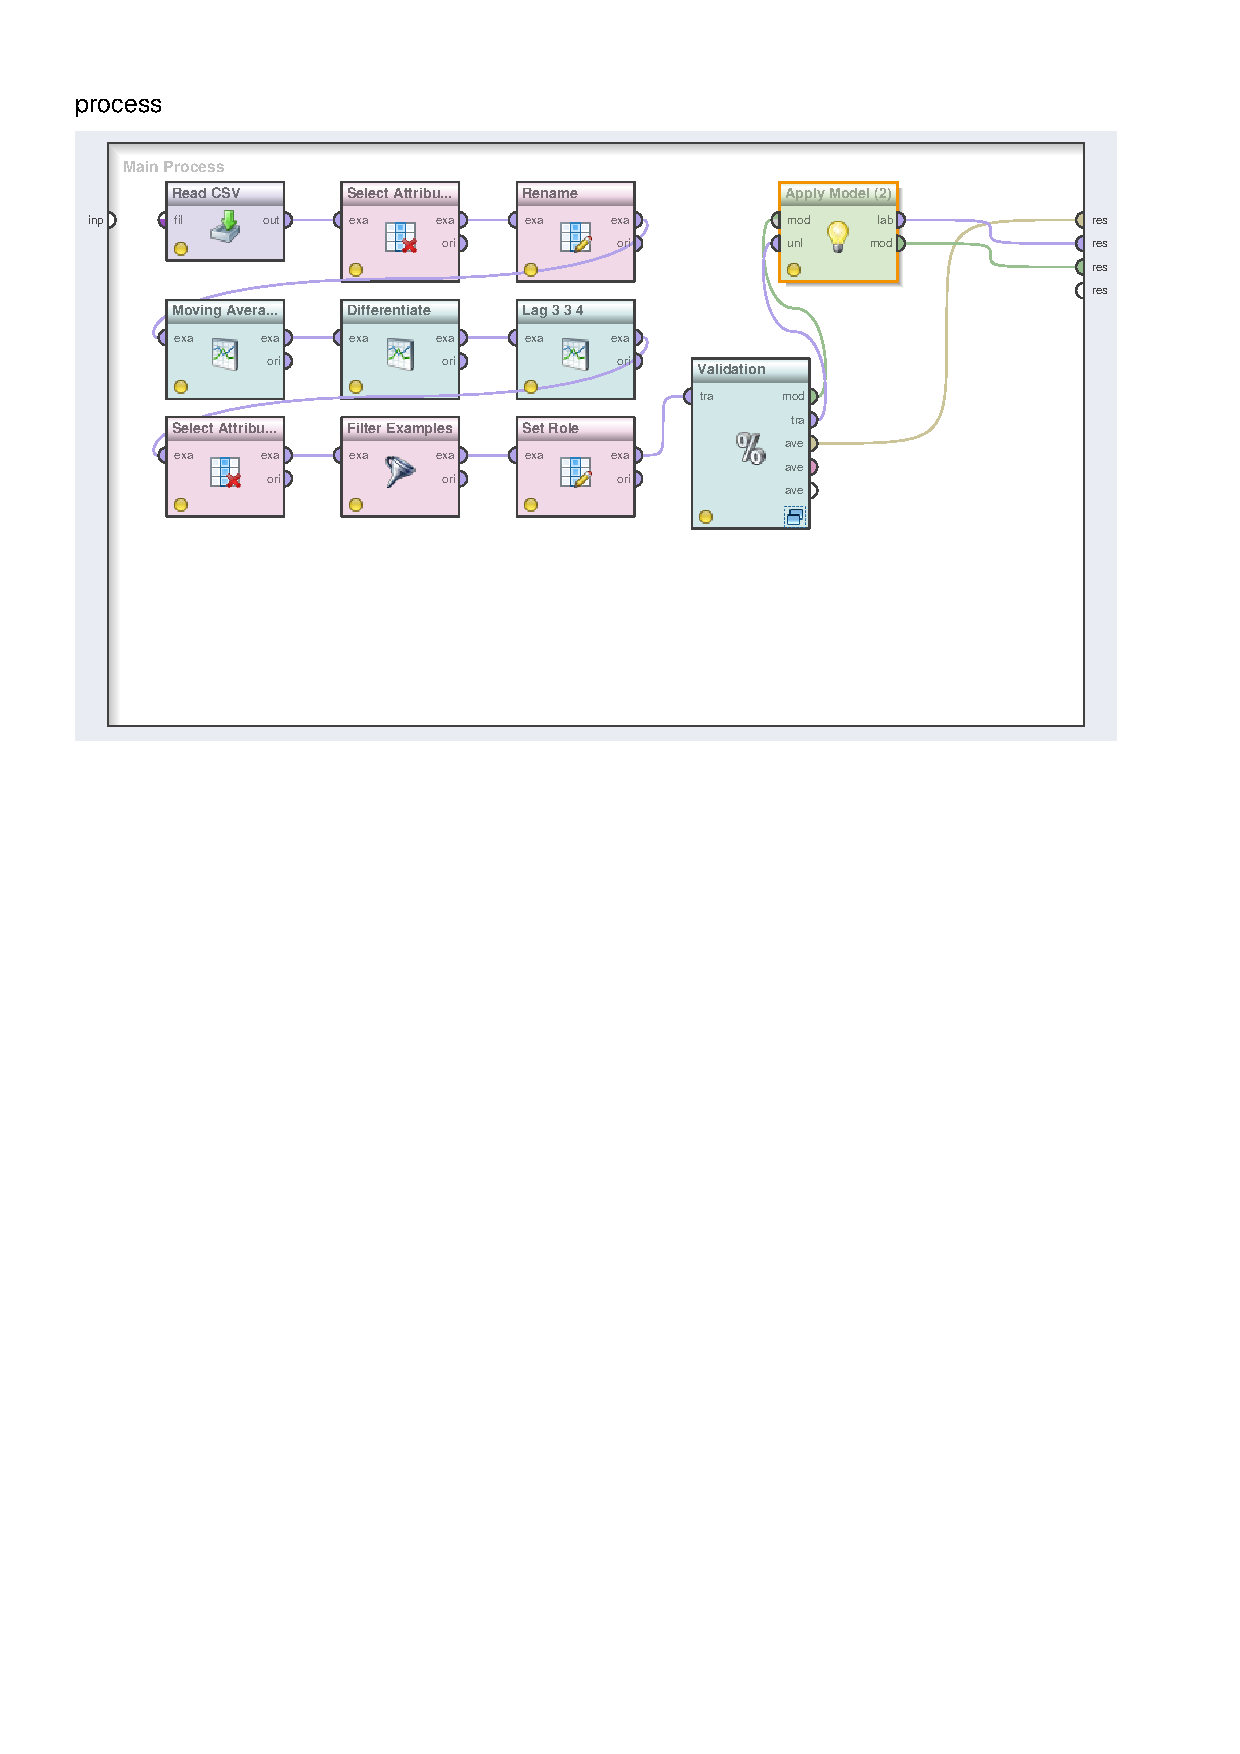
\includegraphics[width=12cm]{../Figures/chp_ts_rm_arima}
\caption[Rapid Miner hybrid ARIMA process]{Rapid Miner hybrid ARIMA process.}
\label{fig:chp_ts_rm_arima}
\end{figure}

Figure \ref{fig:chp_ts_rm_arima_validation} shows the cross-validation operator of the hybrid ARIMA Rapid miner process. This operator can hold alternative learners other than the standard regression operator found in ARIMA models. In the diagram there is an Artificial Neural Network (ANN) operator shown, other options include k-Nearest Neighbour (k-NN) and Support Vector Machine (SVM) operators.

\begin{figure}[h!]
\centering
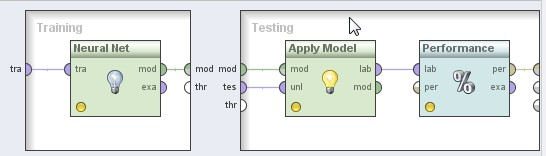
\includegraphics[width=10cm]{../Figures/chp_ts_rm_arima_validation}
\caption[Rapid Miner cross-validation operator]{Rapid Miner cross-validation operator within the hybrid ARIMA process.}
\label{fig:chp_ts_rm_arima_validation}
\end{figure}

Using the hybrid ARIMA methods two types of predictions were carried out. Firstly, in section \ref{sec:pred:cp} the actual closing price of the following observation was predicted, which is a numeric label. This was done by combining ANN and k-NN with ARIMA, as these learners can output numeric class labels. Secondly, in section \ref{sec:pred:ud} the more general situation of whether the market increased or fell in value over the course of the day, was predicted. In this case there are two options, either the market moved up or down. For this second situation a combination of ARIMA with ANN, k-NN and SVM was used, as all three can forecast a binary label.

% ------------------------------------------------------------------------------
\section{Predicting Closing Price}
\label{sec:pred:cp}
As mentioned previously ARIMA and hybrid ARIMA models were used to predict either the value of the one-step ahead close price or the binary value of whether the market moved up or down. In this section the ability of hybrid ARIMA models to forecast the future price of financial markets (as opposed to the general direction up or down) is explored.

\subsection{ARIMA/Artificial Neural Networks (ANN)}
\label{sec:cp_ann}
An ARIMA/ANN method was used to generate predictions for the closing price of the indice data sets under study. As described in section \ref{sec:arima:chp5}, previous values of the label (closing price), along with past values for the difference and moving averages are passed to an ANN learner within a rapid miner process. Artificial Neural Networks can be used to predict categorical or numeric labels, but can only use numeric inputs. They are slow to learn, but their strength lies in their ability to model complex patterns. Essentially they are designed to mimic the human brain by the use of layers of neurons with connections between them. The neurons are found in input and output layers as well as optional hidden layers. The model is constructed by applying weights to the connections which are used to calculate the label.

Rapid miner implements ANN as a feed-forward neural network trained by back propagation. Feed-forward refers to the fact that information only moves forward from the input nodes to the output neurons. Back propagation is an algorithm in which errors are fed back into the system so that the algorithm can adjust the connection weights between nodes until the error converges to some state. Typically the best results were obtained from using a small learning rate and momentum and using a hidden layer of neurons.

For each data set applying the hybrid model produces a new one-step forecast attribute, in a similar manner to the forecast attribute seen in Table \ref{tab:chp_ts:ftse_100_fcast}, which can be used in the System 1 and 2 algorithms previously introduced in section \ref{sec:traing:arima:models}. Table \ref{tab:chp_ts:arima_ann_sys1} are the results generated by passing the output of the ARIMA/ANN models to trading System 1, which compares the previous closing price with the current forecast.

\label{todo:chp5:tab:chp_ts:arima_hybrid_reg}

%label - tab:chp_ts:arima_hybrid_reg
% latex table generated in R 3.1.0 by xtable 1.7-3 package
% Wed Aug 06 18:17:47 2014
\begin{table}[ht]
\centering
\caption[Results from passing closing price predictions from hybrid ARIMA/ANN model to System 1]{Results from passing closing price predictions from hybrid ARIMA/ANN model to System 1.} 
\label{tab:chp_ts:arima_ann_sys1}
\begin{tabular}{lcccccc}
  \toprule Mkt & LongPL & ShortPL & L Win \% & Av L PL & S Win \% & Av S PL \\ 
  \midrule Dax & -5 & -204 & 53 & 0 & 46 & -1 \\ 
  CAC & 355 & 1350 & 56 & 1 & 50 & 2 \\ 
  FTSE & 1692 & 443 & 52 & 2 & 47 & 2 \\ 
  Dow & 2725 & -4100 & 55 & 5 & 44 & -9 \\ 
  Nikkei & 1633 & 2759 & 56 & 6 & 54 & 4 \\ 
  AORD & -898 & -1194 & 52 & -1 & 48 & -4 \\ 
   \bottomrule \end{tabular}
\end{table}


Table \ref{tab:chp_ts:arima_ann_sys2} are the results of passing the output of the ARIMA/ANN models to trading System 2, which compares the value of the current forecast with the previous one.

%label - tab:chp_ts:arima_hybrid_reg
% latex table generated in R 3.1.0 by xtable 1.7-3 package
% Sat Aug 16 11:48:14 2014
\begin{table}[ht]
\centering
\caption[Results from passing closing price predictions from hybrid ARIMA/ANN model to System 2]{Results from passing closing price predictions from hybrid ARIMA/ANN model to System 2.} 
\label{tab:chp_ts:arima_ann_sys2}
\begin{tabular}{lcccccc}
  \toprule Mkt & LongPL & ShortPL & L Win \% & Av L PL & S Win \% & Av S PL \\ 
  \midrule DAX & 3283 & 3110 & 56 & 6 & 49 & 7 \\ 
  CAC & -1832 & -816 & 49 & -3 & 46 & -2 \\ 
  FTSE & 1092 & -182 & 52 & 2 & 48 & 0 \\ 
  Dow & 3829 & -2942 & 54 & 7 & 43 & -7 \\ 
  Nikkei & -4485 & -3229 & 48 & -9 & 50 & -7 \\ 
  AORD & -2783 & -137 & 51 & -5 & 47 & 0 \\ 
   \bottomrule \end{tabular}
\end{table}


\subsection{ARIMA/k-Nearest Neighbour (k-NN)}
An ARIMA/k-NN method was used to generate predictions for the closing price of the indice data sets. The k-Nearest Neighbour algorithm operates by comparing the current set of attributes to others in the data set and finding ones that are \textquotedblleft close" to it. Closeness is usually defined by a distance measure, such as Euclidean, after the attributes have been stored in a n-dimensional pattern space. The k closest neighbours are selected and the most common class of these used to classify the label. In a similar manner to the ANN modelling of section \ref{sec:cp_ann}, lag variables of the close price (label attribute to be forecast), moving average and differences of the close price were passed to a k-NN learner in Rapid Miner in order to predict the one-step ahead forecast. 

The k-NN learner has only a small number of parameters such as k, the number of close neighbours to be considered and the types of measures to be used. Fifteen was found to be a good value for k and either euclidean or cosine similarity a good choice for the distance measure. Table \ref{tab:chp_ts:pred_close_arima_knn_sys1} shows the results of passing data sets containing forecasts generated with the hybrid ARIMA/k-NN to trading System 1. Table \ref{tab:chp_ts:pred_close_arima_knn_sys2} shows the results of passing data sets containing forecasts generated with the hybrid ARIMA/k-NN to trading System 2.

%label - tab:chp_ts:pred_close_arima_knn_sys1
% latex table generated in R 3.1.0 by xtable 1.7-3 package
% Sun Jun 29 08:18:31 2014
\begin{table}[ht]
\centering
\caption[Results from passing closing price predictions from hybrid ARIMA/k-NN model to System 1]{Results from passing closing price predictions from hybrid ARIMA/k-NN model to System 1.} 
\label{tab:chp_ts:pred_close_arima_knn_sys1}
\begin{tabular}{lcccccc}
  \toprule Mkt & LongPL & ShortPL & L Win \% & Av L PL & S Win \% & Av S PL \\ 
  \midrule Dax & 8270 & 9900 & 56 & 4 & 52 & 6 \\ 
  CAC & 6284 & 12597 & 54 & 3 & 55 & 7 \\ 
  FTSE & 17605 & 17026 & 58 & 9 & 56 & 10 \\ 
  Dow & 30330 & 20549 & 59 & 17 & 53 & 12 \\ 
  Nikkei & 15374 & 33366 & 54 & 9 & 57 & 20 \\ 
  AORD & 7658 & 6638 & 57 & 4 & 53 & 4 \\ 
   \bottomrule \end{tabular}
\end{table}


%label - tab:chp_ts:pred_close_arima_knn_sys2
% latex table generated in R 3.1.0 by xtable 1.7-3 package
% Sat Jun 07 08:35:53 2014
\begin{table}[ht]
\centering
\caption[Predicting Close Price - Arima/knn predictions passed to System 2]{Predicting Close Price - Arima/knn predictions passed to System 2} 
\label{tab:chp_ts:pred_close_arima_knn_sys2}
\begin{tabular}{lcccccc}
  \toprule Mkt & LongPL & ShortPL & L Win \% & Av L PL & S Win \% & Av S PL \\ 
  \midrule Dax & 6131 & 7750 & 54 & 3 & 50 & 5 \\ 
  CAC & -567 & 5746 & 50 & 0 & 50 & 3 \\ 
  FTSE & 2571 & 1992 & 52 & 1 & 49 & 1 \\ 
  Dow & 8466 & -1269 & 54 & 4 & 48 & -1 \\ 
  Nikkei & -5066 & 12577 & 49 & -3 & 52 & 8 \\ 
  AORD & 3153 & 2013 & 54 & 2 & 50 & 1 \\ 
   \bottomrule \end{tabular}
\end{table}


% ----------------------------------------------------------------------------------
\section{Predicting Up or Down - Categorical Label}
\label{sec:pred:ud}
In this section the ability of hybrid ARIMA models to forecast whether a financial market will rise or fall is investigated. A categorical attribute taking values \textquotedblleft U" and \textquotedblleft D", representing whether the market moved up (\textquotedblleft U") or down (\textquotedblleft D")  was introduced into the indice data sets depending upon which way the market moved that day. the final six observations of the FTSE data sat with the binary label added can be seen in Table \ref{tab:chp_ts:ftse_100_fcast_ud}. Hybrid ARIMA models using ANN, k-NN and SVM learners, were used to generate one-step ahead forecasts for this categorical label.

\begin{table}[ht]
\centering
\caption[FTSE 100 data set with \textquotedblleft U" and \textquotedblleft D" label]{FTSE 100 data set with \textquotedblleft U" and \textquotedblleft D" label introduced.} 
\label{tab:chp_ts:ftse_100_fcast_ud}
\begin{tabular}{lccccc}
  \toprule Date & Open & High & Low & Close & U/D \\ 
  \midrule 20/12/2013 & 6585 & 6617 & 6577 & 6607 & U \\ 
  23/12/2013 & 6607 & 6679 & 6606 & 6679 & U \\ 
  24/12/2013 & 6679 & 6712 & 6672 & 6694 & U \\ 
  27/12/2013 & 6694 & 6754 & 6694 & 6751 & U \\ 
  30/12/2013 & 6751 & 6768 & 6718 & 6731 & D \\ 
  31/12/2013 & 6731 & 6757 & 6731 & 6749 & U \\ 
   \bottomrule \end{tabular}
\end{table}

\newpage
\subsection{ARIMA/Artificial Neural Networks (ANN)}
\label{sec:ann:ud}
Lag values from the moving average of the closing price, the difference values between consecutive observations and the closing price were passed to an ANN learner to create one-step ahead forecasts of the \textquotedblleft U" and \textquotedblleft D" values. The R code for a trading system using the forecasts from a hybrid model can be seen in Appendix \ref{AppendixA} section \ref{appA:ts_4}. The algorithm simply uses the prediction from the hybrid ARIMA model to decide whether to trade long or short. Table \ref{tab:chp_ts:pUD_CAT_arima_ann_sys} lists the results from the trading system using the hybrid ARIMA/ANN forecasts.

%Parameters:
%Validation - train/test windows, horizon
%ANN - hidden layers, train cycles, learn rate, momentum 

\label{todo:chp5:tab:chp_ts:pUD_CAT_arima_ann_sys}

%label - tab:chp_ts:pUD_CAT_arima_ann_sys
% latex table generated in R 3.1.0 by xtable 1.7-3 package
% Mon Jun 23 18:28:03 2014
\begin{table}[ht]
\centering
\caption[Results from a trading system using the forecast of categorical label "U/D" from hybrid ARIMA/ANN model]{Results from a trading system using the forecast of categorical label "U/D" from hybrid ARIMA/ANN model.} 
\label{tab:chp_ts:pUD_CAT_arima_ann_sys}
\begin{tabular}{lcccccc}
  \toprule Mkt & LongPL & ShortPL & L Win \% & Av L PL & S Win \% & Av S PL \\ 
  \midrule Dax & 49 & 1714 & 56 & 2 & 48 & 0 \\ 
  CAC & 0 & 6426 & NaN & NaN & 50 & 2 \\ 
  FTSE & 7399 & 6806 & 55 & 5 & 51 & 3 \\ 
  Dow & 12434 & 2711 & 56 & 8 & 49 & 1 \\ 
  Nikkei & -14054 & 3771 & 49 & -4 & 56 & 24 \\ 
  AORD & 3938 & 2978 & 53 & 1 & 59 & 13 \\ 
   \bottomrule \end{tabular}
\end{table}


\subsection{ARIMA/k-Nearest Neighbour (k-NN)}
%Parameters:
%Validation - train/test windows, horizon
%k-NN - k = 15
In a similar manner to section \ref{sec:ann:ud}, an ARIMA/k-NN model was also employed in an attempt to predict the categorical label indicating whether the financial markets would move up or down. The forecasts produced from these hybrid models were also applied to the trading algorithms listed in \ref{AppendixA} section \ref{appA:ts_4}. Table \ref{tab:chp_ts:pUD_CAT_arima_knn_sys} lists the trading results from this combination.

%label - tab:chp_ts:pUD_CAT_arima_knn_sys
% latex table generated in R 3.1.0 by xtable 1.7-3 package
% Tue Jul 22 20:47:45 2014
\begin{table}[ht]
\centering
\caption[Results from a trading system using the forecast of categorical label "U/D" from hybrid ARIMA/k-NN model]{Results from a trading system using the forecast of categorical label "U/D" from hybrid ARIMA/k-NN model.} 
\label{tab:chp_ts:pUD_CAT_arima_knn_sys}
\begin{tabular}{lcccccc}
  \toprule Mkt & LongPL & ShortPL & L Win \% & Av L PL & S Win \% & Av S PL \\ 
  \midrule Dax & 15692 & 17357 & 61 & 8 & 60 & 12 \\ 
  CAC & 10161 & 16587 & 60 & 6 & 59 & 9 \\ 
  FTSE & 15553 & 14960 & 60 & 8 & 60 & 10 \\ 
  Dow & 30347 & 20624 & 62 & 14 & 60 & 15 \\ 
  Nikkei & 27206 & 45031 & 60 & 18 & 60 & 24 \\ 
  AORD & 9711 & 8751 & 60 & 5 & 59 & 6 \\ 
   \bottomrule \end{tabular}
\end{table}


As the results from Table \ref{tab:chp_ts:pUD_CAT_arima_knn_sys} were good, the algorithm was re-run but this time a stop loss was introduced. A stop loss of 100 points was applied to all the markets and the amended results can be seen in Table \ref{tab:chp_ts:pUD_CAT_arima_knn_sys_SL}. In a similar manner as encountered previously, the use of the stop loss was beneficial for all the markets except the Dow in which case it had a large detrimental affect.

%label - tab:chp_ts:pUD_CAT_arima_knn_sys_SL
% latex table generated in R 3.1.0 by xtable 1.7-3 package
% Tue Aug 26 19:02:10 2014
\begin{table}[ht]
\centering
\caption[Results from a trading system with a stop loss using the forecast of categorical label "U/D" from hybrid ARIMA/k-NN model]{Results from a trading system with a stop loss using the forecast of categorical label "U/D" from hybrid ARIMA/k-NN model.} 
\label{tab:chp_ts:pUD_CAT_arima_knn_sys_SL}
\begin{tabular}{lcccccc}
  \toprule Mkt & LongPL & ShortPL & L Win \% & Av L PL & S Win \% & Av S PL \\ 
  \midrule DAX & -430 & -1444 & 53 & -1 & 47 & -4 \\ 
  CAC & 203 & 1326 & 52 & 0 & 49 & 2 \\ 
  FTSE & 1919 & 526 & 54 & 4 & 50 & 1 \\ 
  Dow & 5475 & -1922 & 51 & 11 & 42 & -4 \\ 
  Nikkei & 4021 & 2804 & 48 & 9 & 49 & 6 \\ 
  AORD & 570 & 3424 & 53 & 1 & 50 & 7 \\ 
   \bottomrule \end{tabular}
\end{table}


%\subsection{ARIMA / Reg}

\subsection{ARIMA/Support Vector Machine (SVM)}
ARIMA was also married with a SVM learner in order to predict the categorical value, \textquotedblleft U" or \textquotedblleft D". SVMs are linear classifiers that can only operate with binary class labels and thus assign observations in a data set to one of two options, in this case \textquotedblleft U" or \textquotedblleft D". 

\begin{figure}[tbph!]
\centering
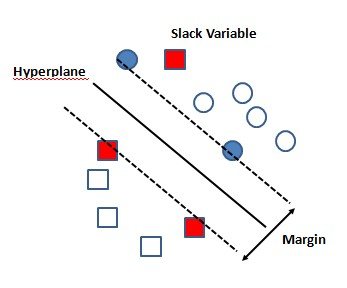
\includegraphics[width=8cm]{SVM}
%\caption{fs yrytrytr}
\caption[SVM margins and slack variables]{SVM margins and slack variables.}
\label{fig:SVM}
\end{figure}

Support vector machines operate by finding the straight line that dissects a data set such that the points close to the dividing line are as far away from it as possible. In high dimensional data sets the dividing lines can be considered as a set of hyperplanes in a high dimensional space. The algorithm works by choosing the hyperplanes that are furthest from the boundary data points, which are known as the support vectors. This intuitively would provide the best classification between two sets of data points. Observations that are classified into the wrong class are known as slack variables, the number of which increases as width of the dividing margin increases. 

Figure \ref{fig:SVM} illustrates the margin calculated from a SVM between two classes of observations, and the presence of a wrongly classified slack variable. Therefore in SVMs there is a trade off between a narrow margin with a small number of slack margins, which could represent over-fitting, and a wider margin with more wrongly classified data points. In the Rapid Miner SVM operator, the parameter \textquotedblleft C" is a cost function, that applies a cost to slack variables. If this parameter is set to a high value there is a high cost applied to the creation of a slack variable and therefore the model produces tight margins and risks over-fitting the model. For low values of C, models with wider margins with more slack variables are produced.

In order to allow for non-linear boundaries between classes non-linear kernel functions are used in SVM. These map the original data set into a data set with a larger number of dimensions which can then be split with a linear function.

Table \ref{tab:chp_ts:pUD_CAT_arima_svm_sys} lists the results of passing forecasts made using hybrid ARIMA/SVM models to the trading algorithm listed in \ref{AppendixA} section \ref{appA:ts_4}. Typically small values were used for the cost parameter in Rapid Miner and a radial non-linear kernel function applied.


%label - tab:chp_ts:pUD_CAT_arima_svm_sys
% latex table generated in R 3.1.0 by xtable 1.7-3 package
% Tue Aug 19 13:19:33 2014
\begin{table}[ht]
\centering
\caption[Results from a trading system using the forecast of categorical label "U/D" from hybrid ARIMA/SVM model]{Results from a trading system using the forecast of categorical label "U/D" from hybrid ARIMA/SVM model.} 
\label{tab:chp_ts:pUD_CAT_arima_svm_sys}
\begin{tabular}{lcccccc}
  \toprule Mkt & LongPL & ShortPL & L Win \% & Av L PL & S Win \% & Av S PL \\ 
  \midrule DAX & -123 & -322 & 53 & 0 & 46 & -1 \\ 
  CAC & -1607 & -612 & 49 & -4 & 47 & -1 \\ 
  FTSE & 2115 & 866 & 54 & 5 & 49 & 1 \\ 
  Dow & 2138 & -4686 & 57 & 10 & 45 & -6 \\ 
  Nikkei & 9 & 1135 & 48 & 0 & 51 & 2 \\ 
  AORD & -2364 & 301 & 53 & -4 & 49 & 1 \\ 
   \bottomrule \end{tabular}
\end{table}


% -------------------------------------------------------------------
%\section{Predicting Up or Down - Continuous Label}
%An alternative to using a categorical variable represented by \textquotedblleft U" or \textquotedblleft D" to indicate if the market rose of fell is to use the numeric range 0 to 1. Here 0 is used to indicate the market fell and 1 to indicate that it increased in value. Thus an additional attribute was introduced into the national indice data sets which took the value of 0 or 1.
%
%\subsection{ARIMA/Artificial Neural Networks (ANN)}
%An ARIMA/ANN model was employed in an attempt to predict the value of 0 or 1, which indicates the directional movement of the market. Table \ref{tab:chp_ts:pUD_01_arima_ann_sys} are the results of passing the indice data sets augmented with the ARIMA/ANN forecasts to the trading algorithm listed in Appendix \ref{AppendixA} section \ref{appA:ts_3a}.
%% EXP algorithm ...
%
%%label - tab:chp_ts:pUD_01_arima_ann_sys
%% latex table generated in R 3.1.0 by xtable 1.7-3 package
% Thu May 29 13:12:22 2014
\begin{table}[ht]
\centering
\caption[Predicting UpDn 01 - Arima/ANN predictions passed to System 2.]{Predicting UpDn 01 - Arima/ANN predictions passed to System 2} 
\label{tab:chp_ts:pUD_01_arima_ann_sys}
\begin{tabular}{lcccccc}
  \toprule Mkt & LongPL & ShortPL & L Win \% & Av L PL & S Win \% & Av S PL \\ 
  \midrule Dax & 316 & 0 & 53 & 0 & NaN & NaN \\ 
   \bottomrule \end{tabular}
\end{table}

%
%\subsection{ARIMA/k-Nearest Neighbour (k-NN)}
%An ARIMA/k-NN model was used to make forecasts for the continuous variable that represents whether the market will move up or down. The output of the model is a value between 0 and 1. The trading algorithm that uses this prediction can be seen in Appendix \ref{AppendixA} section \ref{appA:ts_3} and the results generated in Table \ref{tab:chp_ts:pUD_01_arima_knn_sys}. The trading algorithm looks at the forecast value and trades long if the values are over 0.5 and short if they are below this value.
%
%%label - tab:chp_ts:pUD_01_arima_knn_sys
%% latex table generated in R 3.1.0 by xtable 1.7-3 package
% Sun Jun 29 08:18:37 2014
\begin{table}[ht]
\centering
\caption[Results from a trading system using the forecast of a continous label from a hybrid ARIMA/ANN model]{Results from a trading system using the forecast of a continous label from a hybrid ARIMA/k-NN model.} 
\label{tab:chp_ts:pUD_01_arima_knn_sys}
\begin{tabular}{lcccccc}
  \toprule Mkt & LongPL & ShortPL & L Win \% & Av L PL & S Win \% & Av S PL \\ 
  \midrule Dax & 14122 & 15787 & 64 & 11 & 55 & 7 \\ 
  CAC & 11115 & 17540 & 65 & 10 & 57 & 7 \\ 
  FTSE & 18156 & 17563 & 65 & 14 & 56 & 8 \\ 
  Dow & 28106 & 18383 & 66 & 20 & 55 & 9 \\ 
  Nikkei & 21724 & 39549 & 63 & 25 & 57 & 15 \\ 
  AORD & 9607 & 8647 & 65 & 7 & 56 & 4 \\ 
   \bottomrule \end{tabular}
\end{table}



%\subsection{ARIMA / Regression}
%Using ARIMA with regression to predict 0/1 to represent up and down - See Table \ref{tab:chp_ts:01_arima_reg_sys}
%
%
%%label - tab:chp_ts:01_arima_reg_sys
%% latex table generated in R 3.1.0 by xtable 1.7-3 package
% Fri May 30 21:37:15 2014
\begin{table}[ht]
\centering
\caption[Predicting UpDn 01 - Arima/Reg predictions passed to System 3.]{Predicting UpDn 01 - Arima/Reg predictions passed to System 3} 
\label{tab:chp_ts:01_arima_reg_sys}
\begin{tabular}{lcccccc}
  \toprule Mkt & LongPL & ShortPL & L Win \% & Av L PL & S Win \% & Av S PL \\ 
  \midrule Dax & 749 & 2414 & 53 & 0 & 50 & 4 \\ 
  CAC & 2013 & 8438 & 53 & 1 & 53 & 4 \\ 
  FTSE & 3962 & 3370 & 53 & 2 & 52 & 3 \\ 
  Dow & 13649 & 3925 & 54 & 5 & 52 & 8 \\ 
  Nik & 3633 & 21458 & 52 & 8 & 52 & 7 \\ 
  AORD & 2404 & 1444 & 53 & 1 & 55 & 5 \\ 
   \bottomrule \end{tabular}
\end{table}

 
% Chapter 6

\chapter{Analysis} % Main chapter title

\label{Chapter6} % For referencing the chapter elsewhere, use \ref{Chapter6} 

\lhead{Chapter 6. \emph{Analysis}} % This is for the header on each page - perhaps a shortened title

%----------------------------------------------------------------------------------------

\section{Introduction}
In chapters 4 and 5 a wide variety of analytical techniques were applied to a range of time series data sets. In Chapter 4 a number of trading algorithms were developed based on technical analysis indicators, with the intention of automating the decision of whether to buy or sell a market. For comparison purposes, two simple so called "naive" systems were explored to act as a baseline against which the technical analysis indicators could be compared.  The technical indicators were grouped together into their general area of applicability, namely trend detection indicators, reversal, momentum and candlestick indicators.

Chapter 5 continued the exploration of financial time series through the use of exponential smoothing, ARIMA and hybrid ARIMA techniques. The generated models were used to create one-step ahead forecasts which were then added to the original data sets. These amended data sets were then fed into trading algorithms which used the forecast values to make buying decisions.

\section{Exponential Smoothing}
Exponential smoothing was used to make one step ahead forecasts for the indice data sets. Initially two base systems were explored in order that they could be used as a baseline against which later results could be compared. The two methods generated predictions using a mean method in which the forecast was simply the average of the sample and a drify method which is the extrapolation of a striaght line between the first and last point in a data sample. For all the forecasts generated in this section a moving window approach was adopted. A window of sample data points was used, typically the last 30 observations, for which a forecast was generated using one of the methods. This window was then advanced one observation forward and the forecast for this data set calculated and the process repeated for the entire data set.

Once the forecasts were generated they were passed to a trading algorithm which made decisions regarding whether to trade long or short based on the value of the forecast. If the forecast was higher than the previous closing price a long trade was initiated or if it was lower a short trade was made with the expectation that the market would fall. Results from the forecasts generated from the mean method can be seen in Figure \ref{} while results from the drift method can be seen in Figure \ref{}. Both systems produced poor results and wouldn't generate enough profits to offset any transaction costs that would be incurred in the real world.

Next exponential smoothing was used to  generate forecasts. Allowing for trend, seasonality and whether there are additive or multiplicative affects, a variety of models may be used to generate predictions. The ets() function of the forecast package in R can create models from all the available possibilities. Once again using a moving window approach, one step ahead forecasts were created for the indice data sets. As the window moved through the data, different models were selected as being the best fit and these used to generate the forecasts. Having generated the preditctions they were passed to the same trading algorithm as used for the mean and drift models, and the results can be seen in Figure \ref{}. 

RESULTS in diss are the same as mean model ...


\section{Technical Analysis}

\subsection{Baseline Systems}
Initially two simple, naive systems were explored so that they could be used as a baseline against which the developed predictive models could be compared. These systems were the Naive Long System which mirrors a buy and hold strategy and a Naive Reversing System which simply trades in the opposite direction to the previous days market movement.

The first baseline system tried was the Naive Long system in which a market buy is placed each day and is similar to the so-called \textquotedblleft Buy and Hold" technique. The assumption here is that the market rises over time and if an investor simply holds a security it will eventually generate a profit.  The total profit is the price at the start, in this case the data set started in 2000, subtracted from the price at the end of the period, which in this case was the end of 2013.

The first iteration of the algorithm placed a buy at the start of the trading session and closed it at the end and thus the system was out of the market overnight. This resulted in significant discrepancies from the returns expected from a buy and hold system. Table \ref{tab:ind_start_stop_chp6} lists the expected returns from a Buy and Hold system over this period, with the Difference column being the profit or loss over the time.

% ---------- Table
\begin{table}[!htbp] \centering  
\caption[Returns from a  \textquotedblleft Buy and Hold" technique]{Returns from a  \textquotedblleft Buy and Hold" technique.}
\label{tab:ind_start_stop_chp6}
\begin{tabular}{lcccc}
\toprule
Date & Start 2000 & End 2013 & Difference & \% Change  \\
\midrule
Dax & 6961 & 9552   & +2591 & +37 \\
CAC & 6024 & 4250   & -1774 & -29 \\
FTSE & 6930 & 6749  & -181  & +-3 \\
Dow & 11501 & 16576 & +5075 & +44 \\
Nik & 18937 & 16291 & -2646 & -14 \\
AORD & 3152 & 5353  & +2201 & +70 \\
\bottomrule
\end{tabular}
\end{table}

From simply trading long during market hours the Dax generated a loss as opposed to the 2591 profit expected, likewise the CAC showed a much larger loss than expected and the Nikkei resulted in a large loss when a small loss was expected. The Dow, FTSE and AORD were similar to the expected values. The discrepancies in the returns between the trading algorithm and a Buy and Hold approach was due to
the fact that the algorithm opened and closed trades each day as opposed to simply opening the trade and waiting several years. This first algorithm was simply trading within market hours, approximately 8am to 5pm local time, and was not in the market for the full 24 hours of the day.

Changing the algorithm such that the trades ran from the market close time until the close time of the following day and thus covered the full 24 hour period resulted in system results that matched those expected from a buy and hold approach.  Clearly the discrepancies from the first algorithm were due to the relative amounts the markets moved during the day as opposed to during the \textquotedblleft out of hours" trading. There is a slight bias for the markets to move upwards overnight and over the course of the study (14 years) adds up to significant values.  

The second naive system was termed the \textquotedblleft Naive Reversing" system and simply places a trade today in the opposite direction from the previous day. This idea produced reasonable returns, with every market making money. From these results it can be concluded that the markets have a tendency to "flip flop" and reverse back on themselves, and the phenomena of market reverses is well understood. This second concept produced far better results than the first and was thus used as the primary basis of comparison for the algorithms and systems developed from technical indicators and time series methods. For convenience the results from this system are reproduced in Table \ref{tab:n_rev_results_chp6}.

% \label{tab:n_rev_results_chp6}
% latex table generated in R 3.1.0 by xtable 1.7-3 package
% Fri Jul 11 07:22:22 2014
\begin{table}[ht]
\centering
\caption[Results from the Naive Reversing System.]{Results from a naive trading system which simply trades in the opposite direction to the previous day's movement.} 
\label{tab:n_rev_results_chp6}
\begin{tabular}{lcccccc}
  \toprule Mkt & LongPL & ShortPL & L Win \% & Av L PL & S Win \% & Av S PL \\ 
  \midrule Dax & 947 & 3131 & 53 & 1 & 49 & 2 \\ 
  CAC & 940 & 7810 & 53 & 1 & 53 & 4 \\ 
  FTSE & 4284 & 4115 & 53 & 3 & 50 & 2 \\ 
  Dow & 15799 & 6047 & 56 & 10 & 49 & 3 \\ 
  Nikkei & 2324 & 20486 & 51 & 1 & 54 & 12 \\ 
  AORD & 1264 & 237 & 53 & 1 & 48 & 0 \\ 
   \bottomrule \end{tabular}
\end{table}


%Naive Reversed PL:
%CAC - 7800 (L)
%FTSE - 4000 (LS)
%Dow - 6000/15800
%Nik - 20500(L)

\subsection{Trend Detection}
The first group of the technical analysis indicators studied were the trend detection indicators. Identification of trend direction and strength is very important in the world of financial trading and one of the most widely encountered phrases is "the trend is your friend", as most authorities advocate trading in the direction of the trend. (In fact on a recent webinar it was claimed that 80\% of all money made is made trading in the direction of the trend.)  Well known indicators that purport to assist the trader in identifying trends are the simple moving average (SMA), the moving average convergence/divergence indicator (MACD) and the Aroon indicator.

The use of simple moving average is wide-spread in the financial markets. Market participants track moving averages or even more than one and make a decision which way to trade based on the position of the current price relative to it. Popular values to use in the SMA are 25, 50 and 200 for the look back period. The results of a trading system based on SMA is presented in Table \ref{tab:sma_results} of Chapter \ref{Chapter4}. The algorithm places a buy trade if the current price is above the SMA and a sell trade if it is below it. 

Results are mixed from using the SMA, with some markets producing positive results and some ending in losses. The German Dax and Australian AORD produce positive results across all the SMA values with returns from trading short (predicting the market will decline) doing best.  The Japanese Nikkei and French CAC display different behaviour in that all the SMA values tried produce negative results in trying to  predict long trades but positive returns when attempting to predict short trades.  The UK's FTSE 100 is different again, producing negative results across the board. Finally, the Dow produces positive results for trades on the long side but losses for trading short.

%DOES this reflect on how these markets move? - smooth trends would be profitable ...
%NOTE - worth analysing "trending" behaviour?  Amount of time >70 in aroon?   

In an attempt to improve the returns from the trading system a stop loss was introduced. Comparing Tables \ref{tab:sma_results} and \ref{tab:sma_results_Sloss} of Chapter \ref{Chapter4}
it can be seen that applying the stop loss has been on the whole beneficial to the results obtained, with the exception of those from the Dow which were negatively impacted. Essentially losing trades have been truncated while winning trades have been left to develop. This general pattern of a stop loss being beneficial to all the markets except the US Dow was seen multiple times with the systems tested.

%b. MACD – no SL applied here
The second trend detection indicator explored was the Moving Average Convergence Divergence (MACD) indicator, full details of which can be found in section \ref{appB:MACD} of Appendix \ref{AppendixB}. The MACD can generally be used two ways, as a trend detection indicator and as an over-bought/over-sold indicator in which case traders use it to identify potential market reversals. In this section the indicator was used as a trend detector and the results from a system based on the MACD indicator can be seen in Table \ref{tab:mac_trend_results} in Chapter \ref{Chapter4}.  The algorithm trades long when the value of MACD is greater than the value of the signal line, see Appendix \ref{AppendixA} section \ref{appA:macd_xov} for details of the R code used. The results are not very impressive, only the Nikkei producing reasonable profits, although they wouldn't beat the baseline Naive Reversing system.

The final trend detection indicator examined was Aroon.  This indicator measures the number of intervals since the previous high or low within a certain time window. The algorithms presented here used a time window of 20 days. If the current day was the highest price in the last 20 days trading, the indicator would take a value of 100 and for each following day that doesn't make a new high the indicator falls by 5 (100 divided by the lag period which is 20).  Thus if the highest price was four days ago the AroonUp value would be 80. The opposite situation occurs with regard to the low price. A value of 70 or above for the AroonUp is indicative of a upward trending market and likewise a value of 70 and above for AroonDn suggests a falling market.

The results from an algorithm using the Aroon indicator can be seen in Table \ref{tab:aroon_results} of Chapter \ref{Chapter4}. Overall the results are encouraging with the Dax, FTSE, Dow and AORD all producing positive returns for both long and short trades, while the CAC and Nikkei are positive when trading short. Table \ref{tab:aroon_results_diff} lists the values derived from the Aroon system with those from the baseline Reversing system (see Chapter \ref{Chapter4} section \ref{sec:naive:rev}) subtracted. Because the Aroon system doesn't execute trades each day it only makes sense to compare the average daily returns as opposed to the total returns. As can be seen from  Table \ref{tab:aroon_results_diff}, compared with the baseline system for some markets the Aroon indicator outperforms the baseline while for others it is worse, notably the Nikkei. Considering the second column in Table \ref{tab:aroon_results_diff}, \textquotedblleft Diff in Mean Long PL" only the Dax and AORD outperformed the baseline reversing system in producing long winning trades. Alternatively, the system based on the Aroon indicator was superior in predicting winning short trades for all the markets except the Nikkei, as seen in the third column \textquotedblleft Diff in Mean Short PL".

%\ref{tab:aroon_results_diff}
% latex table generated in R 3.1.0 by xtable 1.7-3 package
% Fri May 30 19:26:05 2014
\begin{table}[ht]
\centering
\caption[Naive Long System - Close to Close]{Naive Long System changed such that the trading period is the previous close price minus today's close.} 
\label{tab:aroon_results_sloss_diff}
\begin{tabular}{lcc}
  \toprule Market & Long Difference & Short Difference \\ 
  \midrule Dax & 102 & 2208 \\ 
  CAC & 414 & 1167 \\ 
  F100 & 49 & 2300 \\ 
  Dow & -18053 & -13152 \\ 
  Nik & 8005 & 10164 \\ 
  Oz & 51 & 619 \\ 
   \bottomrule \end{tabular}
\end{table}


The trading system based on the Aroon indicator was re-run with a stop loss value of 100. Overall the use of a stop loss improves the returns, with the exception of the Dow. One again using a stop loss with the Dow shows very marked negative impacts on profits. These results can be seen in \ref{tab:aroon_results_sloss} of Chapter \ref{Chapter4}.

\subsection{Market Reversal Indicators}
In this section two indicators that purport to assist in identifying market reversals are examined, namely the Parabolic Stop-and-Reverse (SAR) and the Moving Average Convergence Divergence (MACD) used as an over-bought/over-sold indicator. 

The first market reversal indicator explored was the Parabolic Stop-and-Reverse (SAR), an indicator initially developed for traders who were always in the market with either long or short position. The SAR is used to judge when the  position should be reversed from long to short or vice versa. The trading algorithm reported here trades each day (i.e opens a trade at the start of the trading session and closes it out at the end) and makes a decision regarding the direction of the trade based on the SAR indicator. If the market opening is above the SAR a long trade is initiated and vice versa if the market is below the SAR value.

The results from the trading system based on the SAR can be seen in Table \ref{tab:sar_results} of Chapter \ref{Chapter4} and are very poor. Only the Nikkei trading short produces reasonable results, but these are much worse than the baseline Naive Reversing method introduced previously.

As previously mentioned the MACD indicator can be used as a market reversal indicator. Once the MACD value reaches its extreme values, the market is considered over-bought or over-sold and likely to reverse back on itself. The trading algorithm using this concept expects a market reversal once the MACD crosses above the 85\% quantile (of the MACD range) or below the 15\% quantile. Short trades are initiated once the MACD crosses above the 85\% quantile value and short trades once it has passed below the 15\% quantile. The results from this trading system can be seen in Table \ref{tab:mac_ob_results} and are very unimpressive being inferior to the baseline method.

\subsection{Momentum Indicators}
A third category of technical indicators are the momentum indicators, which are related to the trend detection indicators. Two such indicators are studied here, the Stochastic and Rate of Change (ROC). The stochastic oscillator is one of the oldest and most widely used of the technical indicators. It measures the percentage position the current close is in relation to the high low range of the period of interest. For example the current close could be 80\% of the way between the low and high of the last 10 days. Thus it has conceptual similarities to the Aroon indicator. The stochastic is usually represented by two lines \%K which is the position of the price within this high low envelope described above, and \%D a moving average of \%K (see Appendix \ref{AppendixB} section \ref{appB:stoch} for more details). 

The trading algorithm utilising the stochastic initiates long trades when \%K is above \%D and short trades when \%K is below \%D. Results from an algorithm implementing these ideas can be seen in  Table \ref{tab:stoch_results} in Chapter \ref{Chapter4}. The results of this system are poor being significantly worse than the baseline Naive Reversing system. 

%ROC1 - Mkt$Long <- ifelse(Mkt$prevROC < lw,Mkt$Close-Mkt$Open,NA)
%ROC2 - Mkt$Long <- ifelse(Mkt$prevROC > 0,Mkt$Close-Mkt$Open,NA)

The second momentum indicator is the Rate Of Change (ROC) indicator, and this is simply the difference between the current price and a price a certain number of days previously. If this value is positive the market is considered to be trending up and the larger the value the greater the trending momentum. The results from an algorithm using these ideas is presented in Table \ref{tab:stoch_results} of Chapter \ref{Chapter4}. The results are positive but very modest and inferior to the baseline Reversing system.

\subsection{Breakout systems}
The fourth area of technical analysis explored the idea of trade signals being generated by a particular value from the previous day, so-called breakout systems. Two particular values are used as the trigger price for a trade, the previous day's high/low or the 90\% quantile of the minor move (see section \ref{sec:ohol:fluctuation} of Chapter \ref{Chapter3}). 

The first idea explored was to use the previous time period's high or low price as a trigger for a buy or sell. If the current day's high price exceeded the previous day's high price a long trade would be made and in a similar manner if today's low price is lower than previous day's low a short trade is initiated. Results from using the previous day's high price or low price as a trigger to trade long or short can be seen in Table \ref{tab:hl_bout_sys}. Generally the results are very good with the exception of the Dow. These results can be linked to the data exploratory work shown in Table \ref{tab:closeHL} of section \ref{sec:closing_prices}. The best returns were generated in the Nikkei, a market which had the highest number of times closing outside the previous day's high or low. Conversely, the lowest ranked market in terms of closing outside yesterday's high low range was the Dow, and this was the one market that produced negative results in the break-out system. Table \ref{tab:hl_bout_sys_diff} lists the returns from the high low breakout system with the profits from the baseline Naive Reversing system subtracted. As can be seen, with the exception of the Dow, the method out-performs the baseline system markedly.

%lab = 'tab:hl_bout_sys_diff'
% latex table generated in R 3.1.0 by xtable 1.7-3 package
% Tue Jun 10 16:51:55 2014
\begin{table}[ht]
\centering
\caption[Daily High / Low Breakout System compared with Naive Reversing System]{Results from Daily High / Low Breakout System compared with Naive Reversing System} 
\label{ab:hl_bout_sys_diff}
\begin{tabular}{lcccccc}
  \toprule Mkt & LongPL & ShortPL & L Win \% & Av L PL & S Win \% & Av S PL \\ 
  \midrule Dax & 20126 & 18098 & 5 & 10 & 7 & 11 \\ 
  CAC & 13312 & 12366 & 5 & 7 & 6 & 8 \\ 
  FTSE & 8955 & 14499 & 6 & 4 & 9 & 10 \\ 
  Dow & -35154 & -33381 & -14 & -21 & -11 & -20 \\ 
  Nikkei & 72276 & 61159 & 13 & 43 & 10 & 37 \\ 
  AORD & 18083 & 21007 & 14 & 10 & 17 & 14 \\ 
   \bottomrule \end{tabular}
\end{table}


The second break-out system used the minor fluctuation 90\% quantile value as the trigger level to trade long or short. Once the market moved above this level a long trade was made or if the market moved below this level a short trade was executed. Overall this methodology produces good results with the exception of the Dow and CAC. Table \ref{tab:chp_ta_90q_diff} lists the difference in results between this breakout methodology and the baseline Naive Reversing system.

%lab = 'tab:chp_ta_90q_diff'
% latex table generated in R 3.1.0 by xtable 1.7-3 package
% Fri Jul 11 07:22:30 2014
\begin{table}[ht]
\centering
\caption[Daily 90\% Quantile level Breakout System compared with Naive Reversing System]{Results 90\% Quantile level Breakout System compared with Naive Reversing System} 
\label{tab:chp_ta_90q_diff}
\begin{tabular}{lcccccc}
  \toprule Mkt & LongPL & ShortPL & L Win \% & Av L PL & S Win \% & Av S PL \\ 
  \midrule Dax & 6894 & 3240 & 3 & 5 & 4 & 2 \\ 
  CAC & 1707 & -2725 & 1 & 1 & -1 & -1 \\ 
  FTSE & 6474 & 11180 & 3 & 4 & 4 & 8 \\ 
  Dow & -46061 & -40901 & -17 & -34 & -12 & -31 \\ 
  Nikkei & 21282 & 11344 & 7 & 15 & 2 & 8 \\ 
  AORD & 15466 & 19120 & 10 & 8 & 14 & 12 \\ 
   \bottomrule \end{tabular}
\end{table}


\subsection{Candlestick Patterns}
A number of so-called candlestick patterns were explored for predictive properties in financial markets. The patterns tested were essentially market reversal patterns. Firstly, Hammer and Inverted Hammer were considered. When these patterns occur it is considered a sign that the market will move upwards, especially when they are encountered in a down trend, thus reversing direction. Table \ref{tab:hammer_results} lists the results from placing buy trades after all occurrences of either pattern while Table \ref{tab:hammer_aroon_results} shows the results from initiating buy trades when these patterns occur in trending markets. The Aroon indicator detailed in section \ref{appB:aroon} of Appendix \ref{AppendixB} was used to determine if the market was in a trending phase. Overall the results from using the Hammer or Inverted Hammer candlestick pattern to predict market movement was poor. Only the Dow and FTSE showed positive results, although the per trade profit from the Dow was good. Another consideration is the small number of times in which these patterns occur, only 22 trades in the 14 years of the Dow data were made.  Clearly these visual patterns are quite subjective and in reality a trader would use judgement as to whether the pattern constituted a Hammer or not. However, in developing an algorithm to recognise and trade them no such latitude is possible and thus the number of trades taken by the algorithms is likely to be less than in reality.

The next pattern tested was the Engulfing pattern. This pattern occurs when a candlestick has a lower low and a higher high than the previous day's candlestick, it engulfs it. The presence of this pattern it supposed to indicate that the market will change direction. The results of a trading algorithm that trades long or short depending upon the presence of an Engulfing candlestick can be seen in Table \ref{tab:engulf_results}. The results shown in Table \ref{tab:engulf_aroon_results} are similar to Table \ref{tab:engulf_results} except trades are only taken if the market is trending, with the Aroon indicator used to determine if the market is in a trending phase. The results from both algorithms were very poor, with most markets showing negative results.

The final pattern tested was the Doji, one of the best known candlestick patterns. Again the presence of this pattern in a trending market is supposed to give warning to the market participants that a reversal may be imminent. Table \ref{tab:doji_aroon_results} shows the results of a trading system that uses the presence of a Doji in a trending market to initiate a trade. Again the results are very poor with mostly negative returns.

\section{Time Series Analysis}
ARIMA and hybrid ARIMA models were used to generate forecasts of the closing prices and the more general situation of whether the market would rise or fall. In modelling the more general situation of market direction a categorical and a continuous label was employed. The categorical label used \textquotedblleft U" to represent occasions when the market prices increased and \textquotedblleft D" for when it decreased in value. Alternatively the values 1 and 0 were also used to represent up and down respectively. The primary difference between the two labels was in the values returned from the hybrid ARIMA models. When using 1 and 0 for the class label the models return a value in the range of 1 to 0, whereas for the categorical value there was only the choice of the two values. 

\subsection{ARIMA Models}
The auto.arima() function of the R forecast package was used to assist in generating ARIMA models for the national indice data sets used in this study. For convenience the models selected are listed in Table \ref{tab:chp_ts_arima_models_chp6}.

%label - tab:chp_ts_arima_models
% latex table generated in R 3.1.0 by xtable 1.7-3 package
% Sat Aug 16 11:47:58 2014
\begin{table}[ht]
\centering
\caption[ARIMA models chosen for the indice data sets]{ARIMA models chosen to forecast future values in the national indice data sets.} 
\label{tab:chp_ts_arima_models_chp6}
\begin{tabular}{lc}
  \toprule Market & ARIMA Model \\ 
  \midrule DAX & ARIMA(3,1,3)                    \\ 
  CAC & ARIMA(2,1,3)                    \\ 
  FTSE & ARIMA(2,1,3)                    \\ 
  Dow & ARIMA(1,1,2)                    \\ 
  Nikkei & ARIMA(2,1,3)                    \\ 
  AORD & ARIMA(1,1,0)                    \\ 
   \bottomrule \end{tabular}
\end{table}


The one-step forecasts generated from these models were then used in two trading systems. In the first algorithm the decision to trade long or short was dependant upon on the relative values of the previous close price and the forecast. If the forecast was higher than the close price a long trade was entered in the expectation that the market would rise towards the prediction. The opposite situation was expected for when the forecast was lower than the close price. The R code for this first algorithm can be seen in Appendix \ref{AppendixA} section \ref{appA:ts_1} and is labelled system 1.

The second trading algorithm used the relative values of the predictions themselves in order to decide whether to trade long or short. If the current forecast was higher than the previous one a long trade was made and vice versa.  The R code for this second algorithm can be seen in Appendix \ref{AppendixA} section \ref{appA:ts_2} and is labelled system 2.

The results from both systems were poor. The difference in mean PL per trade between the first system based on the auto.arima models (previous close in comparison to forecast) and the mean PL for the Naive Reversing system from section \ref{sec:naive:rev} Chapter \ref{Chapter4} can be seen in Table \ref{tab:chp_ts:arima1_diff}. Most of the results are worse than the naive baseline system except for the French CAC and US Dow when trading long.

%label - tab:chp_ts:arima1_diff
% latex table generated in R 3.1.0 by xtable 1.7-3 package
% Sat Aug 23 08:35:25 2014
\begin{table}[ht]
\centering
\caption[ARIMA system results minus Naive Reversing results]{PL from Naive Reversing system subtracted from results generated by a trading system based on ARIMA forecasts.} 
\label{tab:chp_ts:arima1_diff}
\begin{tabular}{lcc}
  \toprule Mkt & Diff in Mean Long PL & Diff in Mean Short PL \\ 
  \midrule DAX & -6 & -11 \\ 
  CAC & 2 & -3 \\ 
  FTSE & 1 & -3 \\ 
  Dow & -3 & -14 \\ 
  Nikkei & 20 & 1 \\ 
  AORD & 1 & -1 \\ 
   \bottomrule \end{tabular}
\end{table}


\subsection{ARIMA Hybrids - Predicting Closing Price}
Hybrid ARIMA models in which Artificial Neural Networks and k-Nearest Neighbour algorithms were used instead of regression in the ARIMA algorithm were used to predict the closing prices of financial markets, see Chapter \ref{Chapter5} section \ref{sec:arima:chp5} for details.

\subsubsection{ARIMA/Artificial Neural Networks (ANN)}
Overall the use of the models generated from hybrid ARIMA/ANN algorithms to create trading systems was not very successful. The results from passing the indice data sets augmented with a forecast attribute generated by the hybrid ARIMA models can be seen in Tables  \ref{tab:chp_ts:arima_ann_sys1} and \ref{tab:chp_ts:arima_ann_sys2} of Chapter \ref{Chapter5}. System 1 compares the price of the forecast with the price of the previous close and in the event that the prediction is higher than the previous closing price a long trade is entered. The opposite is true when the forecast is lower than the closing price and a short trade is made. System 2 is similar but compares the forecast with the last forecast. In the event that the current prediction is greater than the previous one a long trade is initiated.

Considering the results in Tables \ref{tab:chp_ts:arima_ann_sys1} and \ref{tab:chp_ts:arima_ann_sys2} it can be seen that System 1 outperforms System 2 quite markedly. Even so, the results are quite modest across most of the indices and especially poor for the Dax. The results prove inferior to the baseline Naive Reversing System introduced in \ref{sec:naive:rev} Chapter \ref{Chapter4} as shown in Table \ref{tab:chp_ts:arima_ann_sys1_diff}.

%label - tab:chp_ts:arima_ann_sys1_diff
% latex table generated in R 3.1.0 by xtable 1.7-3 package
% Tue Jul 22 20:47:42 2014
\begin{table}[ht]
\centering
\caption[Arima/ANN predictions passed to System 1 compared to Naive Reversing methodology]{Results from a trading system based on forecasts of closing price generated by the Arima/ANN model compared to baseline Naive Reversing methodology.} 
\label{tab:chp_ts:arima_ann_sys1_diff}
\begin{tabular}{lcc}
  \toprule Mkt & Diff in Mean Long PL & Diff in Mean Short PL \\ 
  \midrule Dax & -1 & 323 \\ 
  CAC & -1 & 1 \\ 
  FTSE & 29 & -2 \\ 
  Dow & -6 & 1 \\ 
  Nikkei & 3 & -6 \\ 
  AORD & 2 & 0 \\ 
   \bottomrule \end{tabular}
\end{table}


\subsubsection{ARIMA/k-Nearest Neighbour (k-NN)}
An alternative to the ARIMA/ANN methodology is to replace ANN with a k-Nearest Neighbour learner. Results from using the forecasts generated in the two trading systems introduced in section \ref{sec:traing:arima:models} can be seen in Tables \ref{tab:chp_ts:pred_close_arima_knn_sys1} and \ref{tab:chp_ts:pred_close_arima_knn_sys2}. The results from System 1 are very good and exceed the baseline Naive Reversing approach. Table \ref{tab:chp_ts:pred_close_arima_knn_sys1_diff} lists the difference in results between those generated with System 1 and the ARIMA/k-NN models and the baseline system. In all cases the hybrid ARIMA model produces superior results.

%label - tab:chp_ts:pred_close_arima_knn_sys1_diff
% latex table generated in R 3.1.0 by xtable 1.7-3 package
% Sat Aug 16 11:48:15 2014
\begin{table}[ht]
\centering
\caption[Mean PL from hybrid ARIMA/k-NN models minus mean PL from Naive Reverse system]{Results from a system using forecasts from a ARIMA/k-NN model with the results of the Naive Reversing System subtracted.} 
\label{tab:chp_ts:pred_close_arima_knn_sys1_diff}
\begin{tabular}{lcccc}
  \toprule Mkt & L Win \% & Av L PL & S Win \% & Av S PL \\ 
  \midrule DAX & -1 & -1 & -4 & -2 \\ 
  CAC & -1 & -2 & -3 & -3 \\ 
  FTSE & 1 & -2 & 0 & -3 \\ 
  Dow & 1 & 1 & -3 & -7 \\ 
  Nikkei & -3 & -1 & -4 & -10 \\ 
  AORD & 0 & 0 & 2 & 7 \\ 
   \bottomrule \end{tabular}
\end{table}


\subsection{ARIMA Hybrids - Predicting Up Down with Categorical Label}
An alternative to forecasting the closing price of a financial market is to predict the general direction it will move in the short term either up or down. To this end an additional categorical label to indicate whether the market increased or fell in value over the course of the day was introduced into the data sets. This new attribute had the value  \textquotedblleft U" if the market increased and \textquotedblleft D" if it decreased. Hybrid ARIMA models were then employed to predict this label.

\subsubsection{ARIMA/Artificial Neural Networks (ANN)}
The first methodology employed was to combine ARIMA with Artificial Neural Networks (ANN) in order to generate a forecast of the categorical label that indicated whether the market increased in value or fell over the course of the day. Once the forecast was generated and added to the data set in the form of a new attribute it was passed to a trading algorithm which based the decision whether to trade long or short on the forecast generated. The R code for the trading algorithm can be seen in Appendix \ref{AppendixA} section \ref{appA:ts_4} and the results generated in Table \ref{tab:chp_ts:pUD_CAT_arima_ann_sys}. Overall the results were poor and inferior to the baseline system used for comparison. 

\subsubsection{ARIMA/k-Nearest Neighbour (k-NN)}
Replacing the ANN learner from the previous section with a k-NN method resulted in far better results.  Table \ref{tab:chp_ts:pUD_CAT_arima_knn_sys} lists the results of passing the forecasts from this combination to the trading algorithm in Appendix \ref{AppendixA} section \ref{appA:ts_4}. Across all the data sets large positive results are recorded. Table \ref{tab:chp_ts:pUD_CAT_arima_knn_sys_diff} lists the difference in results between using this hybrid ARIMA approach and the usual baseline returns. Clearly this methodology produces superior results. Using a stop loss with this system increases the returns from all the markets except the US Dow and these results are listed in Table \ref{tab:chp_ts:pUD_CAT_arima_knn_sys_SL}.

%label - tab:chp_ts:pUD_CAT_arima_knn_sys_diff
% latex table generated in R 3.1.0 by xtable 1.7-3 package
% Tue Jul 22 20:47:45 2014
\begin{table}[ht]
\centering
\caption[Predicting UpDn CAT - Arima/k-NN predictions passed to System 4 - ]{Results from Naive Reversing System subtracted from results generated from predicting Up/Down categorical label using Arima/k-NN.} 
\label{tab:chp_ts:pUD_CAT_arima_knn_sys_diff}
\begin{tabular}{lcccccc}
  \toprule Mkt & LongPL & ShortPL & L Win \% & Av L PL & S Win \% & Av S PL \\ 
  \midrule Dax & 14745 & 14226 & 8 & 7 & 11 & 10 \\ 
  CAC & 9221 & 8777 & 7 & 5 & 6 & 5 \\ 
  FTSE & 11269 & 10845 & 7 & 5 & 10 & 8 \\ 
  Dow & 14548 & 14577 & 6 & 4 & 11 & 12 \\ 
  Nikkei & 24882 & 24545 & 9 & 17 & 6 & 12 \\ 
  AORD & 8447 & 8514 & 7 & 4 & 11 & 6 \\ 
   \bottomrule \end{tabular}
\end{table}


\subsubsection{ARIMA / SVN}

%label - tab:chp_ts:pUD_CAT_arima_svm_sys
% latex table generated in R 3.1.0 by xtable 1.7-3 package
% Tue Aug 19 13:19:33 2014
\begin{table}[ht]
\centering
\caption[Results from a trading system using the forecast of categorical label "U/D" from hybrid ARIMA/SVM model]{Results from a trading system using the forecast of categorical label "U/D" from hybrid ARIMA/SVM model.} 
\label{tab:chp_ts:pUD_CAT_arima_svm_sys}
\begin{tabular}{lcccccc}
  \toprule Mkt & LongPL & ShortPL & L Win \% & Av L PL & S Win \% & Av S PL \\ 
  \midrule DAX & -123 & -322 & 53 & 0 & 46 & -1 \\ 
  CAC & -1607 & -612 & 49 & -4 & 47 & -1 \\ 
  FTSE & 2115 & 866 & 54 & 5 & 49 & 1 \\ 
  Dow & 2138 & -4686 & 57 & 10 & 45 & -6 \\ 
  Nikkei & 9 & 1135 & 48 & 0 & 51 & 2 \\ 
  AORD & -2364 & 301 & 53 & -4 & 49 & 1 \\ 
   \bottomrule \end{tabular}
\end{table}


%\subsection{ARIMA Hybrids - Predicting Up Down with Numeric Label}
%The final approach adopted was to represent whether a financial market moved up or down by using 1 to signify that the market moved up and 0 that it moved down. The implications of using a numeric value is that the forecasts were in a range between these two values. In such circumstances the trading algorithms picked long trades when the prediction were in the upper half of the range.
%
%\subsubsection{ARIMA/Artificial Neural Networks (ANN)}
%An hybrid approach using ARIMA and ANN was used to make one-step forecasts for the future direction of the market, either up (1) or down (0). Table \ref{tab:chp_ts:pUD_01_arima_ann_sys} in Chapter \ref{Chapter5} lists the results of passing the indice data sets augmented with the ARIMA/ANN forecasts to the trading algorithm listed in Appendix \ref{AppendixA} section \ref{appA:ts_3a}.  Overall the results are poor, especially for the Japanese Nikkei trading long and inferior to the Naive Reversing system that is used as a comparative baseline.
%
%\subsubsection{ARIMA/k-Nearest Neighbour (k-NN)}
%Finally a k-Nearest Neighbour (k-NN) learner was used instead of the ANN algorithm. The models were used to calculate the one-step ahead forecast as represented by a numeric value between 0 and 1. The forecast was added to the data sets and passed to the trading listed in Appendix \ref{AppendixA} section \ref{appA:ts_3}. In common with other forecast using the hybrid k-NN approach good results were obtained and these can be seen in Table \ref{tab:chp_ts:pUD_01_arima_knn_sys} of Chapter \ref{Chapter5}. The results are much better than the baseline system which simply trades based on doing the opposite of what happened yesterday. Table \ref{tab:chp_ts:pUD_01_arima_knn_sys_diff} lists the difference in terms of performance between the two systems and is simply the values in  Table \ref{tab:ntfresults} from Chapter \ref{Chapter4} subtracted from the results in Table \ref{tab:chp_ts:pUD_01_arima_knn_sys} from Chapter \ref{Chapter5}.
%
%%label - tab:chp_ts:pUD_01_arima_knn_sys_diff
%% latex table generated in R 3.1.0 by xtable 1.7-3 package
% Mon Jul 07 19:18:18 2014
\begin{table}[ht]
\centering
\caption[Predicting UpDn 01 - Arima/k-NN predictions passed to System 3.]{Results from Naive Reversing System subtracted from results generated from predicting Up/Down Numerical label using Arima/k-NN.} 
\label{tab:chp_ts:pUD_01_arima_knn_sys_diff}
\begin{tabular}{lcccccc}
  \toprule Mkt & LongPL & ShortPL & L Win \% & Av L PL & S Win \% & Av S PL \\ 
  \midrule Dax & 13175 & 12656 & 11 & 10 & 6 & 5 \\ 
  CAC & 10175 & 9730 & 12 & 9 & 4 & 3 \\ 
  FTSE & 13872 & 13448 & 12 & 11 & 6 & 6 \\ 
  Dow & 12307 & 12336 & 10 & 10 & 6 & 6 \\ 
  Nikkei & 19400 & 19063 & 12 & 24 & 3 & 3 \\ 
  AORD & 8343 & 8410 & 12 & 6 & 8 & 4 \\ 
   \bottomrule \end{tabular}
\end{table}




\section{Conclusion}

TA - not much cop -> b/out good, trend Det - Aroon OK, Rev no good ...

2.1.4 - MACD - reported profitability - not me

2.1.5 - Candlesticks - Marshall reported that they don't work, me same, but visual inspection suggests they do ...

\section{Future Work}
candlestick systems -> price 2,,3,4 days ahead?
combining systems
k-NN seems promising
additional markets
 
%% Chapter 7

\chapter{To Do - Not for Thesis} % Main chapter title

\label{Chapter7} % For referencing the chapter elsewhere, use \ref{Chapter7} 

\lhead{Chapter 7. \emph{To Do - Not for Thesis}} % This is for the header on each page - perhaps a shortened title

%----------------------------------------------------------------------------------------


\begin{itemize}
\item - remove date from opening page ...
\item - consistency - long / short
\item - consistency - Nik, FTSE, Oz

\end{itemize}

\section{Chp2}
\begin{itemize}
\item R Code for graphs in own Script
\item - \ref{todo3} - sort out chapter2 - do we need 2 x ACF plots?
\item -> stationary series - coghlan: no seasonality ot trend ...  further additive -> without trend ...
\item - Exp smoothing - relevance?
\end{itemize}

\section{Chp3}
\begin{itemize}
\item R Code for graphs in own Script
\item section \ref{chp1:ta} - Add refs for TA methods mentioned.
\item table check list - cap top, llcccc etc, big cap, sm cap
\item Lane \cite{lane1986using} and williams \cite{williams2011long} \cite{williams1989definitive} - Chp5c - stoch
\item time in trend - aroon, macd, stoch ...
\end{itemize}

\section{Chp4}
\begin{itemize}
\item cosistent - stop loss, stopped out
\item aroon ref, 
\item Candlestick details - move to Appendix for consistency?
\item candlestick systems -> price 2,,3,4 days ahead?
\end{itemize}

\section{Chp5}
\begin{itemize}
\item - ref{todo-Examine ACF / PACF} - - interpret acf graph
\item - \ref{todo:chp5:tab:chp_ts:arima_hybrid_reg} - results?
\item - \ref{todo:chp5:tab:chp_ts:pUD_CAT_arima_ann_sys} - results?
\item combine ud / 01 -> svn
\end{itemize}

\section{App A}
\begin{itemize}
\item - app A - sub titles
\end{itemize}

% OC % times in direction of major
% open nearest prev HL -> % times cross the nearest?

\textquotedblleft participant

 

%----------------------------------------------------------------------------------------
%	THESIS CONTENT - APPENDICES
%----------------------------------------------------------------------------------------

\addtocontents{toc}{\vspace{2em}} % Add a gap in the Contents, for aesthetics

\appendix % Cue to tell LaTeX that the following 'chapters' are Appendices

% Include the appendices of the thesis as separate files from the Appendices folder
% Uncomment the lines as you write the Appendices

% Appendix A

\chapter{R Code} % Main appendix title

\label{AppendixA} % For referencing this appendix elsewhere, use \ref{AppendixA}
\lhead{Appendix A. \emph{R Code}} % This is for the header on each page - perhaps a shortened title

\section{Chapter 4}
The R code used to generate the results and tables in Chapter \ref{Chapter4} is shown in listing \ref{appA:Chp4_R}. This is followed by the individual files containing the algorithms used in the chapter.

\subsection{Chapter 4 Results Generation}
\label{appA:Chp4_R}
\lstinputlisting{RCode/Chapter4.R}

\subsection{Naive Systems}
\subsubsection{Naive Long System}
\label{appA:NaiveLong}
\lstinputlisting{RCode/NaiveLongSystem.R}

\subsubsection{Naive Long System trading close to close}
\label{appA:NaiveLong_2}
\lstinputlisting{RCode/NaiveLongSystem2.R}

\subsubsection{Naive Reversing System}
\label{appA:NaiveFollowPrev}
\lstinputlisting{RCode/NaiveFollowPrev.R}

\subsection{Trend Detection Systems}
\subsubsection{SMA}
\label{appA:SMA_sys}

\lstinputlisting{RCode/SMA_sys.R}

\subsubsection{MACD - trend indicator}

\lstinputlisting{RCode/MACD_XO.R}
\label{appA:macd_xov}

\subsubsection{Aroon trend indicator}
\label{appA:aroon}
\lstinputlisting{RCode/Aroon.R}

\subsection{Market Reversal Indicator}
\subsubsection{SAR reversal indicator}
\label{appA:sar}
\lstinputlisting{RCode/SAR.R}

\subsubsection{MACD as Reversal Indicator}
\lstinputlisting{RCode/MACD_OB.R} % MACD as over-bought indicator
\label{appA:macd_ob}

\subsubsection{Stochastic reversal indicator}
\label{appA:stoch}
\lstinputlisting{RCode/Stoch.R}

\subsubsection{Rate of Change(ROC)}
\label{appA:roc}
\lstinputlisting{RCode/ROC.R}

\subsection{Break Out Systems}
\subsubsection{Break Out}
\label{appA:bout_sys}
\lstinputlisting{RCode/Bout_sys.R}

\subsubsection{90\% Quantile}

\lstinputlisting{RCode/Quant90_sys.R}
\label{appA:bout_Quant90}

\subsection{Candlestick Systems}
#\subsubsection{Hammer and Inverted Hammer}

\lstinputlisting{RCode/Candle_Hammer.R}
\label{appA:Hammer}

\lstinputlisting{RCode/Candle_Hammer_aroon.R}
\label{appA:Hammer_aroon}

\lstinputlisting{RCode/Candle_Engulf.R}
\label{appA:Engulf}

\lstinputlisting{RCode/Candle_Engulf_aroon.R}
\label{appA:Engulf_aroon}

\lstinputlisting{RCode/Candle_Doji_aroon.R}
\label{appA:Doji_aroon}

\section{Chapter 5}
The R code used to generate the results and tables in Chapter \ref{Chapter5} is shown in listing \ref{appA:Chp5_R}. This is followed by the individual files containing the algorithms used in the chapter.

\lstinputlisting{RCode/Chapter5.R}
\label{appA:Chp5_R}

\subsection{System 1}
\lstinputlisting{RCode/ts_1.R}
\label{appA:ts_1}

\subsection{System 2}
\lstinputlisting{RCode/ts_2.R}
\label{appA:ts_2}

\subsection{Categorical Label}
\lstinputlisting{RCode/ts_4.R}
\label{appA:ts_4}

\subsection{Continuous Label}
\lstinputlisting{RCode/ts_3.R}
\label{appA:ts_3}

\subsection{Continuous Label - ARIMA/ANN}
\lstinputlisting{RCode/ts_3a.R}
\label{appA:ts_3a}

\section{Utility Code}
\label{appA:utility}
\lstinputlisting{RCode/Utils.R}

% Appendix B

\chapter{Technical Indicators} % Main appendix title

\label{AppendixB} % For referencing this appendix elsewhere, use \ref{AppendixB}

\lhead{Appendix B. \emph{Technical Indicators}} % This is for the header on each page - perhaps a shortened title


\section{Moving Average Convergence Divergence (MACD)}
\label{appB:MACD}
MACD is a widely used technical indicator which attempts to detect the early stage of a market trend. It is calculated by subtracting a long exponential moving average (EMA) from a shorter one. The EMA is calculated as follows:

\[ EMA(n)_{t} = \dfrac{2}{n+1}(P_{t}-EMA_{t-1}) + EMA_{t-1}\]

Where $ P_{t} $ is the closing price of a market on day $ t $ and $ n $ is the number of periods used in calculating the moving average. MACD itself is calculated as:

\[ MACD_{t} = EMA(s)_{t} - EMA(l)_{t} \]

where $ EMA(s)_{t} $ is the short moving average and $ EMA(l)_{t} $ is the long one. In addition an EMA of the MACD itself is calculated in order to generate trade signals and is often referred to as the \textquotedblleft trigger line". Thus a particular MACD trading rule is often expressed in the form $ MACD(s,l,k) $ where $ s $ is the number of periods of the short EMA, $ l $ the number of periods of the long EMA and $ k $ the period used to average the MACD for the trigger line.

\section{Aroon Indicator}
\label{appB:aroon}

TTR:
Aroon up (down) is the elapsed time, expressed as a percentage, between today and the highest (lowest) price in the last n periods. If today’s price is a new high (low) Aroon up (down) will be 100. Each subsequent period without another new high (low) causes Aroon up (down) to decrease by (1 / n) x 100.

http://www.fmlabs.com/reference/default.htm?url=Aroon.htm:
The word aroon is Sanskrit for "dawn's early light." The Aroon indicator attempts to show when a new trend is dawning. The indicator consists of two lines (Up and Down) that measure how long it has been since the highest high/lowest low has occurred within an n period range.

When the Aroon Up is staying between 70 and 100 then it indicates an upward trend. When the Aroon Down is staying between 70 and 100 then it indicates an downward trend. A strong upward trend is indicated when the Aroon Up is above 70 while the Aroon Down is below 30. Likewise, a strong downward trend is indicated when the Aroon Down is above 70 while the Aroon Up is below 30. Also look for crossovers. When the Aroon Down crosses above the Aroon Up, it indicates a weakening of the upward trend (and vice versa).

http://www.linnsoft.com/tour/techind/aroon.htm:
Chande states that when AroonUp and AroonDown are moving lower in close proximity, it signals a consolidation phase is under way and no strong trend is evident. When AroonUp dips below 50, it indicates that the current trend has lost its upwards momentum. Similarly, when AroonDown dips below 50, the current downtrend has lost its momentum. Values above 70 indicate a strong trend in the same direction as the Aroon (up or down) is under way. Values below 30 indicate that a strong trend in the opposite direction is underway.

The Aroon Oscillator signals an upward trend is underway when it is above zero and a downward trend is underway when it falls below zero. The farther away the oscillator is from the zero line, the stronger the trend.


\[ Aroon Up = 100 * \left( \dfrac{n - PeriodSinceHighestHigh}{n} \right) \]

\[ Aroon Down = 100 * \left( \dfrac{n - PeriodSinceLowestLow}{n} \right) \]

%\cite{aroon_stockcharts}

\section{Parabolic Stop-and-Reverse (SAR)}
\label{appB:sar}
%http://stockcharts.com/school/doku.php?id=chart_school:technical_indicators:parabolic_sar
The Parabolic Stop-and-Reverse (SAR) is a quite complex indicator developed by Welles Wilder in 1978 \citep{wilder1978new}. The calculation for SAR in rising and falling markets are different and are usually presented separately.

If the market is rising SAR is calculated as:
\begin{center}
Current SAR = Prior SAR + Prior AF(Prior EP - Prior SAR)
\end{center}

where:\\
\begin{itemize}
\item Prior SAR is the SAR value for the previous time period, for example the previous day's value.
\item Extreme Point (EP) is the highest high of the current trend.
\item Acceleration Factor (AF) starts at 0.02, and increases by 0.02 each time the market makes a new high (Extreme Point). The maximum value the AF can reach is 0.20, at which point it is capped.
\end{itemize}
Note:  SAR can never be greater than the value of the previous two periods' lows. Should SAR be above one of those lows, it is set to the lowest of the two.

If the market is falling SAR is calculated as:
\begin{center}
Current SAR = Prior SAR - Prior AF(Prior SAR - Prior EP)
\end{center}
Note:  SAR can never be less than the value of the previous two periods' highs. Should SAR be less than one of those highs, it is set to the lowest of the two.

\section{Stochastic}
\label{appB:stoch}
The stochastic oscillator measures where a particular close price is in relation to the highest high and lowest low in the range under study. It is usually drawn on a chart as two lines, one is \%K and the other is its moving average usually called \%D.

The calculation of the stochastic involves four variables:
\begin{enumerate}
\item \%K Period - the number of periods used in the calculation (see below).
\item \%K Slowing Period - smoothing period applied to \%K.
\item \%D Period - the number of time periods used in the moving average of \%K to generate \%D.
\item \%D Method - the moving average method used to calculate \%D.
\end{enumerate}

\%K is calculated as follows: 

\[ \%K = 100 * \left( \dfrac{\text{Today's Close} - \text{Lowest Low in n Periods}}{\text{Highest High in n Periods} - \text{Lowest Low in n Periods}} \right) \]

The stochastic is used in a variety of ways. One popular method is to buy when the stochastic falls below a particular level then rises back above that level (and vice versa for a short trade). An alternative technique is to buy when the \%K rises above \%D and sell when it falls under \%K.

\section{Rate of Change(ROC)}
\label{appB:roc}
The Rate of Change or ROC indicator highlights the difference between a particular price (e.g. closing price) and the same price a number of periods previously. This value can be expressed in absolute terms or a percentage rise or fall. The calculation is as follows: 

\[ ROC = 100 * \left( \dfrac{ \text{Today's Close} - \text{Today's Close n Periods Ago}}{\text{Today's Close n Periods Ago}} \right) \]

The ROC can be calculated from a wide range of time periods, with 12 and 25 days being the most common. The ROC is typically used as an over-bought / over-sold indicator to provide evidence for when a market turn maybe expected.
% Appendix C

\chapter{Summary of Results} % Main appendix title

\label{AppendixC} % For referencing this appendix elsewhere, use \ref{AppendixB}

\lhead{Appendix C. \emph{Summary of Results}} % This is for the header on each page - perhaps a shortened title


\section{Chapter 4 Results}

% \label{tab:chp6:dax_summary}
% latex table generated in R 3.1.0 by xtable 1.7-3 package
% Sat Aug 16 11:48:17 2014
\begin{table}[ht]
\centering
\caption[Chapter 5 DAX Results]{Chapter 5 DAX Results} 
\label{tab:chp6:dax2_summary}
\begin{tabular}{lcccc}
  \toprule Methodology & LongPL & ShortPL & Av L PL & Av S PL \\ 
  \midrule Mean Method & -1640 & -1505 & -1 & -1 \\ 
  Drift Method & 2310 & 2445 & 1 & 2 \\ 
  Exponential Smoothing & -2029 & -1894 & -1 & -1 \\ 
  ARIMA - System 1 & -1285 & -2522 & -5 & -9 \\ 
  ARIMA - System 2 & 733 & -505 & 3 & -2 \\ 
  ARIMA/ANN Closing Price System 1 & -446 & -645 & -1 & -2 \\ 
  ARIMA/ANN Closing Price System 2 & 3283 & 3110 & 6 & 7 \\ 
  ARIMA/k-NN Closing Price System 1 & 12 & -174 & 0 & 0 \\ 
  ARIMA/k-NN Closing Price System 2 & 489 & 731 & 1 & 2 \\ 
  ARIMA/ANN Up/Down & 199 & 0 & 0 & NaN \\ 
  ARIMA/k-NN Up/Down & -1553 & -1752 & -3 & -4 \\ 
  ARIMA/ANN Up/Down Stop Loss & -430 & -1444 & -1 & -4 \\ 
  ARIMA/SVM Up/Down & -123 & -322 & 0 & -1 \\ 
   \bottomrule \end{tabular}
\end{table}


\newpage
% \label{tab:chp6:cac_summary}
% latex table generated in R 3.1.0 by xtable 1.7-3 package
% Sun Aug 31 09:29:34 2014
\begin{table}[ht]
\centering
\caption[Chapter 4 CAC Results]{Chapter 4 CAC Results} 
\label{tab:chp6:cac_summary}
\begin{tabular}{lcccc}
  \toprule Methodology & LongPL & ShortPL & Av L PL & Av S PL \\ 
  \midrule Naive Long & -6725 & 0 & -2 & 0 \\ 
  Naive Long 2 & -1667 & 0 & 0 & 0 \\ 
  Reverse Prev & 940 & 7810 & 1 & 4 \\ 
  Reverse Prev Stop Loss & 1335 & 8165 & 1 & 5 \\ 
  SMA 5 & -3952 & 2338 & -2 & 1 \\ 
  SMA 25 & -5058 & 1615 & -2 & 1 \\ 
  SMA 50 & -5323 & 1029 & -3 & 1 \\ 
  SMA 100 & -2363 & 3188 & -1 & 2 \\ 
  SMA 200 & -1219 & 3923 & -1 & 3 \\ 
  SMA 100 & -172 & 5178 & 0 & 4 \\ 
  SMA 100 & -1822 & 4658 & -1 & 3 \\ 
  MACD & -4153 & 2188 & -2 & 1 \\ 
  Aroon & -1638 & 4919 & -1 & 4 \\ 
  Aroon Stop Loss & -1224 & 6086 & -1 & 5 \\ 
  SAR & -5584 & 1034 & -3 & 1 \\ 
  MACD Reversal & -545 & 2657 & -1 & 5 \\ 
  Stoch & -4540 & 1817 & -3 & 1 \\ 
  Stoch Stop Loss & -3493 & 2730 & -2 & 2 \\ 
  ROC & 952 & 956 & 2 & 2 \\ 
  Daily Breakout & 3491 & 6955 & 2 & 4 \\ 
  90\% Quantile Breakout & 2647 & 5085 & 2 & 3 \\ 
  Hammer Candlestick & -793 & 0 & -5 & 0 \\ 
  Engulfing Candlestick & -319 & 228 & -2 & 1 \\ 
  Engulfing Candlestick in Trend & -118 & -666 & -3 & -11 \\ 
  Doji Candlestick & -747 & -326 & -6 & -2 \\ 
   \bottomrule \end{tabular}
\end{table}


\newpage
% \label{tab:chp6:ftse_summary}
% latex table generated in R 3.1.0 by xtable 1.7-3 package
% Tue Aug 19 13:20:00 2014
\begin{table}[ht]
\centering
\caption[Chapter 4 FTSE Results]{Chapter 4 FTSE Results} 
\label{tab:chp6:ftse_summary}
\begin{tabular}{lcccc}
  \toprule Methodology & LongPL & ShortPL & Av L PL & Av S PL \\ 
  \midrule Naive Long & 149 & 0 & 0 & 0 \\ 
  Naive Long 2 & 86 & 0 & 0 & 0 \\ 
  Reverse Prev & 4284 & 4115 & 3 & 2 \\ 
  Reverse Prev Stop Loss & 5537 & 5200 & 3 & 3 \\ 
  SMA 5 & -4724 & -5331 & -2 & -3 \\ 
  SMA 25 & -1013 & -1940 & 0 & -1 \\ 
  SMA 50 & -2226 & -2769 & -1 & -2 \\ 
  SMA 100 & -889 & -1692 & 0 & -1 \\ 
  SMA 200 & -158 & -835 & 0 & -1 \\ 
  SMA 100 & 1114 & 6303 & 1 & 5 \\ 
  SMA 100 & -885 & 1892 & 0 & 1 \\ 
  MACD & 63 & -839 & 0 & 0 \\ 
  Aroon & 3042 & 5715 & 2 & 5 \\ 
  Aroon Stop Loss & 3091 & 8015 & 2 & 7 \\ 
  SAR & -1141 & -1663 & -1 & -1 \\ 
  MACD Reversal & 2080 & 1649 & 4 & 3 \\ 
  Stoch & -73 & -744 & 0 & 0 \\ 
  Stoch Stop Loss & 1640 & 1424 & 1 & 1 \\ 
  ROC & 1147 & 1880 & 2 & 4 \\ 
  Daily Breakout & 13189 & 18481 & 7 & 12 \\ 
  90\% Quantile Breakout & 10758 & 15295 & 7 & 10 \\ 
  Hammer Candlestick & 834 & 0 & 4 & 0 \\ 
  Engulfing Candlestick & -1721 & 1185 & -4 & 3 \\ 
  Engulfing Candlestick in Trend & -1217 & -782 & -8 & -3 \\ 
  Doji Candlestick & -697 & 418 & -8 & 3 \\ 
   \bottomrule \end{tabular}
\end{table}


\newpage
% \label{tab:chp6:dow_summary}
% latex table generated in R 3.1.0 by xtable 1.7-3 package
% Tue Aug 19 13:20:00 2014
\begin{table}[ht]
\centering
\caption[Chapter 4 Dow Results]{Chapter 4 Dow Results} 
\label{tab:chp6:dow_summary}
\begin{tabular}{lcccc}
  \toprule Methodology & LongPL & ShortPL & Av L PL & Av S PL \\ 
  \midrule Naive Long & 9816 & 0 & 3 & 0 \\ 
  Naive Long 2 & 5219 & 0 & 1 & 0 \\ 
  Reverse Prev & 15799 & 6047 & 10 & 3 \\ 
  Reverse Prev Stop Loss & -8571 & -14604 & -5 & -8 \\ 
  SMA 5 & 408 & -9630 & 0 & -6 \\ 
  SMA 25 & 1138 & -9204 & 1 & -7 \\ 
  SMA 50 & 5478 & -5876 & 3 & -4 \\ 
  SMA 100 & 2576 & -8220 & 1 & -6 \\ 
  SMA 200 & 6378 & -4567 & 3 & -4 \\ 
  SMA 100 & -18212 & -8229 & -9 & -6 \\ 
  SMA 100 & -11771 & -14696 & -6 & -11 \\ 
  MACD & 5592 & -5190 & 3 & -3 \\ 
  Aroon & 12131 & 3811 & 7 & 3 \\ 
  Aroon Stop Loss & -5922 & -9341 & -3 & -8 \\ 
  SAR & -1301 & -11112 & -1 & -7 \\ 
  MACD Reversal & 3882 & -807 & 7 & -2 \\ 
  Stoch & 867 & -9414 & 0 & -5 \\ 
  Stoch Stop Loss & -13969 & -27388 & -8 & -16 \\ 
  ROC & 8517 & 3396 & 16 & 6 \\ 
  Daily Breakout & -19598 & -28337 & -11 & -17 \\ 
  90\% Quantile Breakout & -30262 & -34854 & -24 & -28 \\ 
  Hammer Candlestick & 2097 & 0 & 24 & 0 \\ 
  Engulfing Candlestick & -770 & -3662 & -4 & -28 \\ 
  Engulfing Candlestick in Trend & 202 & -1154 & 4 & -11 \\ 
  Doji Candlestick & -763 & -2869 & -5 & -10 \\ 
   \bottomrule \end{tabular}
\end{table}


\newpage
% \label{tab:chp6:nik_summary}
% latex table generated in R 3.1.0 by xtable 1.7-3 package
% Fri Jul 11 07:22:35 2014
\begin{table}[ht]
\centering
\caption[Chapter 4 Nikkei Results]{Chapter 4 Nikkei Results} 
\label{tab:chp6:nik_summary}
\begin{tabular}{lcccc}
  \toprule Methodology & LongPL & ShortPL & Av L PL & Av S PL \\ 
  \midrule Naive Long & -18125 & 0 & -5 & 0 \\ 
  Naive Long 2 & -2712 & 0 & -1 & 0 \\ 
  Reverse Prev & 2324 & 20486 & 1 & 12 \\ 
  Reverse Prev Stop Loss & 18137 & 27909 & 10 & 17 \\ 
  SMA 5 & 3078 & 20401 & 2 & 13 \\ 
  SMA 25 & -7878 & 10770 & -4 & 7 \\ 
  SMA 50 & -6054 & 11408 & -4 & 7 \\ 
  SMA 100 & -6235 & 8381 & -4 & 5 \\ 
  SMA 200 & -5928 & 6836 & -4 & 4 \\ 
  SMA 100 Stop Loss & 8258 & 33882 & 5 & 20 \\ 
  SMA 100 Stop Loss & 2550 & 25582 & 2 & 15 \\ 
  MACD & -4078 & 14064 & -2 & 8 \\ 
  Aroon & -4852 & 12013 & -3 & 10 \\ 
  Aroon Stop Loss & 3153 & 22177 & 2 & 18 \\ 
  SAR & -5767 & 12424 & -3 & 8 \\ 
  MACD Reversal & 199 & 2828 & 0 & 6 \\ 
  Stoch & -10591 & 7802 & -6 & 5 \\ 
  Stoch Stop Loss & 1647 & 17977 & 1 & 10 \\ 
  ROC & 2971 & 2546 & 6 & 5 \\ 
  Daily Breakout & 31988 & 43554 & 19 & 27 \\ 
  90\% Quantile Breakout & 23606 & 31830 & 16 & 20 \\ 
  Hammer Candlestick & -2202 & 0 & -15 & 0 \\ 
  Engulfing Candlestick & -3823 & -1166 & -39 & -11 \\ 
  Engulfing Candlestick in Trend & -1522 & -1733 & -59 & -32 \\ 
  Doji Candlestick & 1296 & -2944 & 12 & -22 \\ 
   \bottomrule \end{tabular}
\end{table}


\newpage
% \label{tab:chp6:aord_summary}
% latex table generated in R 3.1.0 by xtable 1.7-3 package
% Mon Jul 14 19:48:31 2014
\begin{table}[ht]
\centering
\caption[Chapter 4 AORD Results]{Chapter 4 AORD Results} 
\label{tab:chp6:aord_summary}
\begin{tabular}{lcccc}
  \toprule Methodology & LongPL & ShortPL & Av L PL & Av S PL \\ 
  \midrule Naive Long & 972 & 0 & 0 & 0 \\ 
  Naive Long 2 & 2229 & 0 & 1 & 0 \\ 
  Reverse Prev & 1264 & 237 & 1 & 0 \\ 
  Reverse Prev Stop Loss & 2320 & 1085 & 1 & 1 \\ 
  SMA 5 & 5009 & 3929 & 3 & 3 \\ 
  SMA 25 & 3701 & 2674 & 2 & 2 \\ 
  SMA 50 & 2804 & 1864 & 1 & 1 \\ 
  SMA 100 & 2688 & 1521 & 1 & 1 \\ 
  SMA 200 & 2574 & 1616 & 1 & 2 \\ 
  SMA 100 & 4008 & 3730 & 2 & 3 \\ 
  SMA 100 & 2881 & 2149 & 1 & 2 \\ 
  MACD & 2563 & 1569 & 1 & 1 \\ 
  Aroon & 3735 & 3540 & 2 & 3 \\ 
  Aroon Stop Loss & 3786 & 4159 & 2 & 4 \\ 
  SAR & 2071 & 1097 & 1 & 1 \\ 
  MACD Reversal & -319 & -584 & -1 & -1 \\ 
  Stoch & 2839 & 1780 & 2 & 1 \\ 
  Stoch Stop Loss & 3028 & 1974 & 2 & 1 \\ 
  ROC & 271 & 1325 & 1 & 2 \\ 
  Daily Breakout & 17225 & 19184 & 10 & 13 \\ 
  90\% Quantile Breakout & 16730 & 19357 & 9 & 12 \\ 
  Hammer Candlestick & -809 & 0 & -3 & 0 \\ 
  Engulfing Candlestick & -6 & -600 & 0 & -3 \\ 
  Engulfing Candlestick in Trend & -49 & -27 & -1 & 0 \\ 
  Doji Candlestick & -115 & 195 & -1 & 2 \\ 
   \bottomrule \end{tabular}
\end{table}


\newpage
\section{Chapter 5 Results}

% \label{tab:chp6:dax_summary}
% latex table generated in R 3.1.0 by xtable 1.7-3 package
% Sat Aug 16 11:48:17 2014
\begin{table}[ht]
\centering
\caption[Chapter 5 DAX Results]{Chapter 5 DAX Results} 
\label{tab:chp6:dax2_summary}
\begin{tabular}{lcccc}
  \toprule Methodology & LongPL & ShortPL & Av L PL & Av S PL \\ 
  \midrule Mean Method & -1640 & -1505 & -1 & -1 \\ 
  Drift Method & 2310 & 2445 & 1 & 2 \\ 
  Exponential Smoothing & -2029 & -1894 & -1 & -1 \\ 
  ARIMA - System 1 & -1285 & -2522 & -5 & -9 \\ 
  ARIMA - System 2 & 733 & -505 & 3 & -2 \\ 
  ARIMA/ANN Closing Price System 1 & -446 & -645 & -1 & -2 \\ 
  ARIMA/ANN Closing Price System 2 & 3283 & 3110 & 6 & 7 \\ 
  ARIMA/k-NN Closing Price System 1 & 12 & -174 & 0 & 0 \\ 
  ARIMA/k-NN Closing Price System 2 & 489 & 731 & 1 & 2 \\ 
  ARIMA/ANN Up/Down & 199 & 0 & 0 & NaN \\ 
  ARIMA/k-NN Up/Down & -1553 & -1752 & -3 & -4 \\ 
  ARIMA/ANN Up/Down Stop Loss & -430 & -1444 & -1 & -4 \\ 
  ARIMA/SVM Up/Down & -123 & -322 & 0 & -1 \\ 
   \bottomrule \end{tabular}
\end{table}


%\newpage
% \label{tab:chp6:cac_summary}
% latex table generated in R 3.1.0 by xtable 1.7-3 package
% Thu Jul 10 21:10:56 2014
\begin{table}[ht]
\centering
\caption[Chapter 5 CAC Results]{Chapter 5 CAC Results} 
\label{tab:chp6:cac2_summary}
\begin{tabular}{lcccc}
  \toprule Methodology & LongPL & ShortPL & Av L PL & Av S PL \\ 
  \midrule Mean Method & -1086 & 3553 & -1 & 2 \\ 
  Drift Method & -2422 & 2217 & -1 & 2 \\ 
  Exponential Smoothing & -266 & 4048 & 0 & 2 \\ 
  ARIMA - System 1 & 1555 & 850 & 6 & 3 \\ 
  ARIMA - System 2 & -76 & -781 & 0 & -3 \\ 
  ARIMA/ANN Closing Price & -1018 & 5295 & 0 & 5 \\ 
  ARIMA/ANN Closing Price System 2 & -5544 & 769 & -3 & 0 \\ 
  ARIMA/k-NN Closing Price & 6284 & 12597 & 3 & 7 \\ 
  ARIMA/k-NN Closing Price System 2 & -567 & 5746 & 0 & 3 \\ 
  ARIMA/ANN Up/Down & 0 & 6426 & NaN & 2 \\ 
  ARIMA/k-NN Up/Down & 10161 & 16587 & 6 & 9 \\ 
  ARIMA/ANN Up/Down Stop Loss & 10524 & 17378 & 6 & 9 \\ 
  ARIMA/SVM Up/Down & 1044 & 7470 & 1 & 4 \\ 
   \bottomrule \end{tabular}
\end{table}


%\newpage
% \label{tab:chp6:ftse_summary}
% latex table generated in R 3.1.0 by xtable 1.7-3 package
% Mon Aug 11 20:47:58 2014
\begin{table}[ht]
\centering
\caption[Chapter 5 FTSE Results]{Chapter 5 FTSE Results} 
\label{tab:chp6:ftse2_summary}
\begin{tabular}{lcccc}
  \toprule Methodology & LongPL & ShortPL & Av L PL & Av S PL \\ 
  \midrule Mean Method & 1680 & 345 & 1 & 0 \\ 
  Drift Method & -518 & -1853 & 0 & -1 \\ 
  Exponential Smoothing & 3866 & 2531 & 3 & 2 \\ 
  ARIMA - System 1 & 990 & -249 & 4 & -1 \\ 
  ARIMA - System 2 & 941 & -383 & 3 & -2 \\ 
  ARIMA/ANN Closing Price System 1 & 625 & -624 & 1 & -2 \\ 
  ARIMA/ANN Closing Price System 2 & 1092 & -182 & 2 & 0 \\ 
  ARIMA/k-NN Closing Price System 1 & 699 & -550 & 1 & -1 \\ 
  ARIMA/k-NN Closing Price System 2 & -388 & -1662 & -1 & -4 \\ 
  ARIMA/ANN Up/Down & 1400 & 151 & 2 & 0 \\ 
  ARIMA/k-NN Up/Down & -266 & -1515 & -1 & -3 \\ 
  ARIMA/ANN Up/Down Stop Loss & 81 & -1162 & 0 & -2 \\ 
  ARIMA/SVM Up/Down & 2115 & 866 & 5 & 1 \\ 
   \bottomrule \end{tabular}
\end{table}


%\newpage
% \label{tab:chp6:dow_summary}
% latex table generated in R 3.1.0 by xtable 1.7-3 package
% Thu Jul 10 21:10:56 2014
\begin{table}[ht]
\centering
\caption[Chapter 5 Dow Results]{Chapter 5 Dow Results} 
\label{tab:chp6:dow2_summary}
\begin{tabular}{lcccc}
  \toprule Methodology & LongPL & ShortPL & Av L PL & Av S PL \\ 
  \midrule Mean Method & 8356 & -2126 & 7 & -1 \\ 
  Drift Method & 5416 & -5066 & 3 & -4 \\ 
  Exponential Smoothing & 12901 & 2419 & 8 & 2 \\ 
  ARIMA - System 1 & 3130 & -1766 & 14 & -6 \\ 
  ARIMA - System 2 & 2910 & -1985 & 10 & -9 \\ 
  ARIMA/ANN Closing Price & 11685 & 1904 & 4 & 4 \\ 
  ARIMA/ANN Closing Price System 2 & -3417 & -13198 & -2 & -8 \\ 
  ARIMA/k-NN Closing Price & 30330 & 20549 & 17 & 12 \\ 
  ARIMA/k-NN Closing Price System 2 & 8466 & -1269 & 4 & -1 \\ 
  ARIMA/ANN Up/Down & 12434 & 2711 & 8 & 1 \\ 
  ARIMA/k-NN Up/Down & 30347 & 20624 & 14 & 15 \\ 
  ARIMA/ANN Up/Down Stop Loss & 7152 & -671 & 3 & 0 \\ 
  ARIMA/SVM Up/Down & 4659 & -5065 & 3 & -3 \\ 
   \bottomrule \end{tabular}
\end{table}


5\newpage
% \label{tab:chp6:nik_summary}
% latex table generated in R 3.1.0 by xtable 1.7-3 package
% Sat Aug 16 11:48:17 2014
\begin{table}[ht]
\centering
\caption[Chapter 5 Nikkei Results]{Chapter 5 Nikkei Results} 
\label{tab:chp6:nik2_summary}
\begin{tabular}{lcccc}
  \toprule Methodology & LongPL & ShortPL & Av L PL & Av S PL \\ 
  \midrule Mean Method & -32 & 10646 & 0 & 6 \\ 
  Drift Method & -6939 & 3739 & -4 & 3 \\ 
  Exponential Smoothing & -2741 & 7937 & -2 & 5 \\ 
  ARIMA - System 1 & 4268 & 3071 & 21 & 13 \\ 
  ARIMA - System 2 & 179 & -916 & 1 & -4 \\ 
  ARIMA/ANN Closing Price System 1 & 913 & 2039 & 2 & 4 \\ 
  ARIMA/ANN Closing Price System 2 & -4485 & -3229 & -9 & -7 \\ 
  ARIMA/k-NN Closing Price System 1 & -66 & 1060 & 0 & 2 \\ 
  ARIMA/k-NN Closing Price System 2 & -2916 & -1660 & -6 & -4 \\ 
  ARIMA/ANN Up/Down & 234 & 1360 & 12 & 1 \\ 
  ARIMA/k-NN Up/Down & 2707 & 3834 & 6 & 8 \\ 
  ARIMA/ANN Up/Down Stop Loss & 4021 & 2804 & 9 & 6 \\ 
  ARIMA/SVM Up/Down & 9 & 1135 & 0 & 2 \\ 
   \bottomrule \end{tabular}
\end{table}


%\newpage
% \label{tab:chp6:aord_summary}
% latex table generated in R 3.1.0 by xtable 1.7-3 package
% Mon Aug 11 20:47:58 2014
\begin{table}[ht]
\centering
\caption[Chapter 5 AORD Results]{Chapter 5 AORD Results} 
\label{tab:chp6:aord2_summary}
\begin{tabular}{lcccc}
  \toprule Methodology & LongPL & ShortPL & Av L PL & Av S PL \\ 
  \midrule Mean Method & -1333 & -2149 & -1 & -1 \\ 
  Drift Method & 1476 & 660 & 1 & 1 \\ 
  Exponential Smoothing & 645 & -171 & 0 & 0 \\ 
  ARIMA - System 1 & 635 & -247 & 2 & -1 \\ 
  ARIMA - System 2 & 811 & -117 & 3 & 0 \\ 
  ARIMA/ANN Closing Price System 1 & -3036 & -371 & -5 & -1 \\ 
  ARIMA/ANN Closing Price System 2 & -2783 & -137 & -5 & 0 \\ 
  ARIMA/k-NN Closing Price System 1 & 497 & 3162 & 1 & 7 \\ 
  ARIMA/k-NN Closing Price System 2 & -3449 & -804 & -6 & -2 \\ 
  ARIMA/ANN Up/Down & -2712 & -47 & -3 & -12 \\ 
  ARIMA/k-NN Up/Down & -2445 & 220 & -4 & 1 \\ 
  ARIMA/ANN Up/Down Stop Loss & 254 & 245 & 0 & 1 \\ 
  ARIMA/SVM Up/Down & -2364 & 301 & -4 & 1 \\ 
   \bottomrule \end{tabular}
\end{table}


\addtocontents{toc}{\vspace{2em}} % Add a gap in the Contents, for aesthetics

\backmatter

%----------------------------------------------------------------------------------------
%	BIBLIOGRAPHY
%----------------------------------------------------------------------------------------

\label{Bibliography}

\lhead{\emph{Bibliography}} % Change the page header to say "Bibliography"

\bibliographystyle{my_plainnat}
%\bibliographystyle{unsrtnat} % Use the "unsrtnat" BibTeX style for formatting the Bibliography

\bibliography{Bibliography_thesis} % The references (bibliography) information are stored in the file named "Bibliography_theses.bib"

\end{document}  